\documentclass{atlasnote} 

%\documentclass[usetikz]{atlasnote} % the 'usetikz' option loads tikz.sty in the proper place, 
                                   % avoiding conflicts with graphicx.sty.
                                   % Don't know what tikz.st is? Just ignore this line! :-)

%\documentclass[coverpage]{atlasnote} % the 'coverpage' option loads the ATLAS Cover Page package 
                                      % ans makes sure that the cover page is generated before the
                                      % note title page. Make sure that the latest version of
                                      % of 'atlascover.sty. is installed on your system!

%\usepackage{graphicx} % This is already loaded by the atlasnote class
                       % Just use it to include your plots!

\usepackage{atlasphysics} % Contains useful shortcuts. Uncomment to use
%%%%%%%%%%%%%%%%%%%%%%%%%%%%%%%%%%%%
%           Title page             % 
%%%%%%%%%%%%%%%%%%%%%%%%%%%%%%%%%%%%

\skipbeforetitle{100pt}

% \atlasnote{ATLAS-PHYS-PUB-2013-005} 

% Title
\title{Supporting Internal Appendices for Comparison of Monte Carlo generator predictions for the fragmentation and decay of heavy flavor hadrons}
%
% Author
%if not given, typesets ``The ATLAS collaboration''
\author{The ATLAS Collaboration}

% if multiple authors/affiliations are needed, use the authblk package
\usepackage{authblk}
\usepackage{subfig}
\usepackage{float}
\renewcommand\Authands{, } % avoid ``. and'' for last author
\renewcommand\Affilfont{\itshape\small} % affiliation formatting

\author[a]{Jacquelyn Brosamer}
\author[a]{Marjorie Shapiro}
%\author[b]{Third Author}
\setcounter{tocdepth}{4} 
\setcounter{secnumdepth}{4} 

\affil[a]{Lawrence Berkeley National Lab}
%\affil[b]{Another Institution}

% Date: if not given, uses current date
%\date{\today}

% Draft version: if given, adds draft version on front page, a
% 'DRAFT' box on top of each other page, and line numbers to easy
% commenting. Comment or remove in final version.
\draftversion{0.3}

% Journal: adds a 
%\journal{} 
%% Defines 
\usepackage{listings}
\usepackage{color}
\usepackage{caption}

\definecolor{dkgreen}{rgb}{0,0.6,0}
\definecolor{gray}{rgb}{0.5,0.5,0.5}
\definecolor{mauve}{rgb}{0.58,0,0.82}

\lstset{frame=tb,
  language=Python,
  aboveskip=3mm,
  belowskip=3mm,
  showstringspaces=false,
  columns=flexible,
  basicstyle={\small\ttfamily},
  numbers=none,
  numberstyle=\tiny\color{gray},
  keywordstyle=\color{blue},
  commentstyle=\color{dkgreen},
  stringstyle=\color{mauve},
  breaklines=true,
  breakatwhitespace=true
  tabsize=3
}


\DeclareCaptionFont{white}{ \color{white} }
\DeclareCaptionFormat{listing}{
  \colorbox[cmyk]{0.43, 0.35, 0.35,0.01 }{
    \parbox{\textwidth}{\hspace{15pt}#1#2#3}
  }
}
\captionsetup[lstlisting]{ format=listing, labelfont=white, textfont=white, singlelinecheck=false, margin=0pt, font={bf,footnotesize} }
\newcommand{\lumi}{\ensuremath{\mathcal L}}
\newcommand{\micr}{\ensuremath{\rm{{\mu}m}}}
\newcommand{\degree}{^{\circ}}
\newcommand{\invpb}  {\ensuremath{\mbox{pb}^{-1}}}
\newcommand{\invfb}  {\ensuremath{\mbox{fb}^{-1}}}
\newcommand{\mbarn}  {\ensuremath{\rm \,mb}} 

\def\pp{\ensuremath{pp}}
\def\mm{\ifmmode  {\mathrm{\ mm}}\else
                   \textrm{~mm}\fi}%
\def\drHadJet{\ensuremath{\Delta R_{\rm\;(hadron, jet)}}}
\def\drHadHad{\ensuremath{\Delta R_{\rm\;(hadron, hadron)}}}
\def\drCC{\ensuremath{\Delta R_{(C, C)}}}
\def\drBB{\ensuremath{\Delta R_{(B,B)}}}
\def\ptHad{\ensuremath{p_T^{\rm\;hadron}}}
\def\ptJet{\ensuremath{p_T^{\rm\;jet}}}
\def\antiktfour{anti-$k_t(R=0.4)$}
\def\antikt{anti-$k_t$}
\def\Dzero{\ensuremath{D^{0}}}
\def\Dplus{\ensuremath{D^{+}}}
\def\Ds{\ensuremath{D_{s}}}
\def\Bo{\ensuremath{B^{0}}}
\def\Bp{\ensuremath{B^{+}}}
\def\Bs{\ensuremath{B_{s}^{0}}}
\def\Lc{\ensuremath{\Lambda_c}}
\def\Lb{\ensuremath{\Lambda_b}}
\def\\ttbar{\ensuremath{t\overline t}}
\def\PythiaEE{Pythia}
\def\PythiaE{Pythia8}
\def\PythiaS{\textsc{Pythia}}
\def\Pythia{\textsc{Pythia6}}
\def\Sherpa{\textsc{Sherpa}}
\def\Herwig{\textsc{Herwig}}
\def\Herwigpp{{Herwig\raise0.2ex\hbox{\scriptsize\kern-0.5pt+\kern-0.5pt+}}}
\def\PowHeg{\textsc{Powheg}}
\def\MCatNLO{\textsc{MC@NLO}}
\def\Jimmy{\textsc{Jimmy}}
\def\Alpgen{\textsc{Alpgen}}
\def\aMCatNLO{aMC@NLO}
\def\EvtGen{EvtGen}
\def\CT{\textsc{CT10}}
\def\MSTW{\textsc{MSTW2008}}
\def\HERA{\textsc{HERA\-PDF1.5}}
\def\epWZ{ATLAS-epWZ12}
\def\NNPDF{\textsc{NNPDF2.3}}
\def\NNPDFcoll{\textsc{NNPDF2.3coll}}
\def\Tauola{\textsc{Tauola}}
\def\Photos{\textsc{Photos}}

% Abstract
\abstracttext{\noindent \textit{Supporting internal appendices for note ATL-COM-PHYS-2014-288, which has the following abstract:}






The fragmentation and decay of heavy flavor hadrons are studied
for four Monte Carlo generators: \PythiaE, \Pythia, \Herwig\ and \Herwigpp.
Heavy flavor production fractions and fragmentation functions are
studied using top-quark pair and high transverse
momentum QCD jet samples generated for $pp$ collisions at $\sqrt{s}=8$~\TeV.  
The performance of the generators for heavy flavor fragmentation is also validated
using $e^+e^-$ annihilation events generated at $\sqrt{s}=91.2$~\GeV\
(for b-quarks) and $\sqrt{s}=10.53$~\GeV\ (for \textit{c}-quarks).  
In addition, charm and bottom hadron decays studied for the four generators and are compared
to both those obtained using the \EvtGen\ Monte Carlo and to experimental measurements. 
}

\begin{document}

% Test of tikz.sty loadin in atlasnote.cls. Use 'usetkiz' option in documentclass declaration:
% e.g. \documentclass[usetikz]{atlasnote}
% \input{tikz-test}
%\section{Introduction}
%\label{sec:intro}
%Final states that include heavy flavor (bottom and charm) hadrons are important for the
study of many processes at the Large Hadron Collider (LHC).  Examples of such processes
include top quark pair (\ttbar) production, Higgs production (with decay to a bottom quark pair)
and searches for signals from physics beyond the Standard Model (SM).  
To fully exploit the large data samples that will be collected during Run II at the LHC,
a reduction in current systematic uncertainties associated with the modeling of
heavy flavor hadron production and decay will be needed.
Although data-driven methods are likely to play a major part in the effort to reduce these
uncertainties, improvementsin the Monte Carlo (MC) models used to determine
reconstruction efficiencies  will also be necessary.

An overview of the physics of general purpose MC event generators can be found in reviews such as References~\cite{Buckley:2011ms} and~\cite{PDGMC}. Simulation of QCD processes using these generators involves four separate stages.  First, the short distance cross section for the process of interest is calculated from the hard-scattering matrix elements obtained using a fixed-order perturbative QCD calculation.    Second, perturbative contributions from initial- and final-state parton showers are included.  These stages together provide a descripiton of the kinematic properties of quarks, gluons and leptons.  Third, soft hadronic phenomena are treated using QCD-inspired models.  In this step, the quarks and gluons are transformed into colorless objects using a hadronization model which includes the effects of fragmentation and soft gluon radiation.  The most common hadronization models are the string model (used by \Pythia~\cite{Sjostrand:2006za} and \PythiaE~\cite{Sjostrand:2007gs}) and the cluster model (used by \Herwig~\cite{Corcella:2002jc} and \Herwigpp~\cite{Bahr:2008pv}).     For hadronic initial states, the underlying event and effects from multiple parton interactions are incorporated at this stage.  The generators all include adjustable phenomenological parameters that are determined by comparing MC predictions to experimental data.  Differences in the treatment of the soft physics and in the values chosen for the adjustable parameters can lead to substantial variations in the kinematic properties of the particles produced (see, for example, the results compiled in Reference~\cite{Karneyeu:2013aha}).  Fourth, hadron and $\tau$ decays proceed according to particle tables that have been adapted from experimental data.




This note presents a study of heavy flavor hadron production and decay properties for four
MC generators (\PythiaE, \Pythia, \Herwigpp\  and \Herwig)  extensively used to 
model \pp\ interactions at the LHC.  Two benchmark physics processes are used for
these comparisons:  \ttbar\ production, in which a $b$-quark is produced in each top
decay and a $c$-quark is produced in approximately 1/3 of the $W$ decays~\footnote{Although
bottom and charm hadrons can also be produced in the parton shower, the rate for such
production is small when compared to that produced in the top decays.}  and
high transverse momentum (\pT) jet production, in which the generators produce
$b$- and $c$-quarks via both the matrix element calculation and the parton shower.  
In addition, ancillary 
$e^+e^-\rightarrow b\overline b$  and $e^+e^-\rightarrow c\overline c$ samples are generated using 
shower parameterizations consistent with those used for LHC tunes.  These samples are used to 
check the consistency of the fragmentation functions with data for the processes in which the
fragmentation functions were originally measured.


The note is organized as follows.  Section~\ref{sec:mcsamples} provides information on the 
configuration of the MC generators used for these studies. 
Section~\ref{sec:prod} presents
the bottom and charm hadron production fractions obtained with these generators and compares them
to world averages of experimental data.  
These production fractions are sensitive to the adjustable parameters of the hadronization model.
Section~\ref{sec:frag} provides a detailed study of the modeling of heavy quark fragmentation.  
The MC generators all rely on the assumption that non-perturbative fragmentation 
functions are universal (aside from the QCD scaling violations).
Section~\ref{sec:decay} compares 
decay properties of heavy flavor hadrons in each of the four generators to world average experimental data.
In addition, these results are compared to those obtained with the
\EvtGen~\cite{Lange:2001uf} decay package, which implements detailed models of flavor decay and
uses branching fraction measurements compiled in Reference~\cite{PhysRevD.86.010001}.
Section~\ref{sec:conclusion} provides a brief summary of the results presented here.


%\section{Monte Carlo Samples}
%\label{sec:mcsamples}
%%MC samples are used to study the effect of different showering generators on the kinematics and decay properties of 
%heavy flavor hadrons produced in \ttbar\ and di-jet events. 

The versions of the four generators studied here are 
\PythiaS\ 6.427, 
\PythiaEE\ 8.175, 
\Herwig\ 6.520 
with \Jimmy\ 4.31~\cite{Butterworth:1996zw} for the underlying event and
\Herwigpp\ 2.6.3a.
All \pp\ samples have been generated with a center-of-mass energy of $\sqrt{s}=8$~\TeV.  

Two physics
processes are studied:
\begin{itemize}

  \item Top-pair production (\ttbar ) is calculated using  
\PowHeg\ ~\cite{Nason:2004rx, Frixione:2007vw, Alioli:2010xd, Alioli:2008gx} r2330 and
the \textsc{CT10}~\cite{Lai:2010vv} parton distribution functions (PDFs).  At keast one of the $W$ bosons in the \ttbar\ event is required to decay leptonically.
The output of \PowHeg\ are files in Les Houches Event (LHE) format, which contain the top-pair decay products (leptons and
quarks). The same 
\PowHeg\ LHE files are then passed to each of the four generators 
for parton shower, hadronization and underlying-event modeling.
The generator tunes used are
Perugia 2011C~\cite{Skands:2010ak} (\Pythia ),
AU2(CT10)~\cite{ATL-PHYS-PUB-2012-003} (\PythiaE )~\footnote{
While the default release of Pythia 8.175 uses the tau lifetimes specified in the \PowHeg\ LHE files, a patch was applied to overrule the incorrect lifetimes written out in the \PowHeg\ event record. This patch has since become part of \PythiaEE~8.175.},
%While the default release of \PythiaEE~8.175 did not
%properly set the $\tau$ lifetime, a patch to fix this problem was applied to the samples studied here.
AUET2(CT10)~\cite{ATL-PHYS-PUB-2011-008} (\Jimmy)
and UE-EE-4-LO**~\cite{Seymour:2013qka} (\Herwigpp ).  
In \Pythia\ and \PythiaE, heavy quark fragmentation uses the Lund symmetric model with
the Bowler modification~\cite{Bowler:1981sb}.  In \Herwig\ and \Herwigpp, heavy quarks are fragmented using the cluster model. 

\item High \pT~jet samples are generated using the matrix
element calculations provided by each generator.  The generator tunes and fragmentation models used are
the same as those used for the \ttbar\ samples. Events are required
to have at least one jet with \pT\ between 500~\GeV\ and 1~\TeV.

\end{itemize}


For both processes, jets are reconstructed from stable particles~\footnote{Stable particles are defined as those with a mean lifetime, $c\tau_{0}$,~$< 10$~mm.} using the
infrared- and collinear-safe \antikt\ algorithm~\cite{bib:antikt2}
with radius parameter $R=0.4$ using the FastJet package~\cite{bib:antikt3}. In the case of \ttbar\ samples, leptons
from the W decay are excluded from the jet recontruction.


For the fragmentation studies in Section~\ref{sec:fragmentation},~$e^+e^-$ samples are generated.
%\Pythia, \PythiaE, \Herwigpp and \Herwig. 
Unless otherwise stated, 
these samples are generated with initial state QED radiation enabled. 
Comparisons with LEP and SLC data use $e^+e^-\rightarrow b\overline{b}$ samples
generated at $\sqrt{s}=91.2$ GeV. In addition, $e^+e^-\rightarrow b\overline{b}$ samples
generated at $\sqrt{s}=200$ GeV with initial state QED disabled for comparison to the $\sqrt{s}=91.2$ GeV samples. Comparisons with Belle and CLEO data are studied using  
$e^+e^-\rightarrow c\overline{c}$ samples with $\sqrt{s}=10.53$ GeV.

%The decay properties of bottom and charm hadrons for the four generators are studied  
%and are compared
For studies of bottom and charm hadron decay properties, \EvtGen~2.0~\cite{Lange:2001uf} is used.
Decay products of all heavy flavor hadrons are removed from the event record and the four-momenta
of the heavy flavor hadrons are passed to \EvtGen, which redecays these hadrons; these new decay
products are added to the event record.
In some cases, modifications to the \EvtGen\ default decay table have been made.  These changes
are discussed in Section~\ref{sec:decay}.

%\section{Heavy Flavor Production Fractions}
%\label{sec:prod}
%
The relative rates for production of different heavy flavor species depend on each
generator's choice of hadronization model and the values of the tunable parameters of that model.
These production fractions have been studied for weakly decaying bottom and charm hadrons in both the \ttbar\
and the high \pT\ jet samples. Results for the \ttbar\ are shown here; the difference between
production fractions in the two processes is less than  0.006.

Figure~\ref{fig:prodfrac} compares the
production fractions for weakly decaying bottom and charm hadrons:

\begin{eqnarray*}
B^{0}\; B^{+}\; B_{s}^{0}\; B_{c}^{+}\; \Lambda_{b}^{0}\; \Xi_{b}^{-}\; \Xi_{b}^{0}\; \Omega_{b}\; D^{+}\; D^{0}\; D_{s}^{+}\; \Lambda_{c}^{+}\; \Xi_{c}^{+}\; \Xi_{c}^{0}\; \Omega_{c}^{0}
\end{eqnarray*} 

\noindent
and their charge conjugates for the four generators.
%in \PythiaE\, \Pythia\, \Herwigpp\ and \Herwig. 
Charm hadron production fractions include only those hadrons produced directly (not from bottom hadron decays).
Although the $\Sigma_B$ should not decay weakly, 
\Herwig\ erroneously decays them weakly under some conditions; these decays are shown on the plot. 
%Differences between the generators are as large as  5-10\%.

%Production fractions for bottom hadrons have larger uncertainties than those for charm hadrons,
%due in part to uncertainties in the baryon fractions.
Recent results from LHCb constrain the ratio of $B_s$ production to $B^0$ production to be
$f_s/f_d = 0.259 \pm 0.015$~\cite{lhcb,fsfb}, with no evidence of dependence 
on the \pT\ or $\eta$ of the hadrons.
%LHCb also constrains the ratio of the $\Lambda_B$ baryon to light be
However, the baryon fraction in the forward region is observed to depend significantly on the  
\pT\ and $\eta$ of the hadron~\cite{lhcb,lam}.  Thus, results from LHCb are of limited use in
constraining baryon production at central rapidities. 

%%which is independent of $f_{\Lambda_B}/(f_u+f_d)= 0.404\pm (0017(stat)\pm0.027(syst)\pm0.105(BR))$. 
The PDG~\cite{PhysRevD.86.010001} provides values for the bottom hadron production fractions at high energy, 

using results obtained from  $Z$ decays and central $p\overline p $ collisions, under the
assumption that these fractions should be universal aside from forward, leading-particle effects
in hadron collisions.
Fractions obtained from the four generators are compared to the PDG values
in Table~\ref{t:bfractions}.
All the generators are in reasonable agreement with the data, although the baryon
fraction in  \PythiaE\ is low.  

For the case of charm hadrons, the experimental data have been
compiled and averaged, including a careful treatment of 
correlated systematic uncertainties in Reference~\cite{r:ffrac}.
Results for the different generators are compared to these averages
in Table~\ref{t:cfractions}.
In general, the generators overestimate the $D^+$ fraction. The $D^0$ fraction
in \Herwig\ is significantly lower than the fraction in the data and other three generators.
Charm baryon fractions 
are poorly constrained by the data and vary widely among the generators.
%These differences in production fractions
%will directly affect the predicted rate for a charm hadron to be tagged as a bottom hadron because the different charm species have significantly different
%lifetimes and semileptonic branching fractions.
%should be give the hadron fractions....right?


\begin{figure}
\centering
\begin{subfigure}[]{0.5\textwidth}
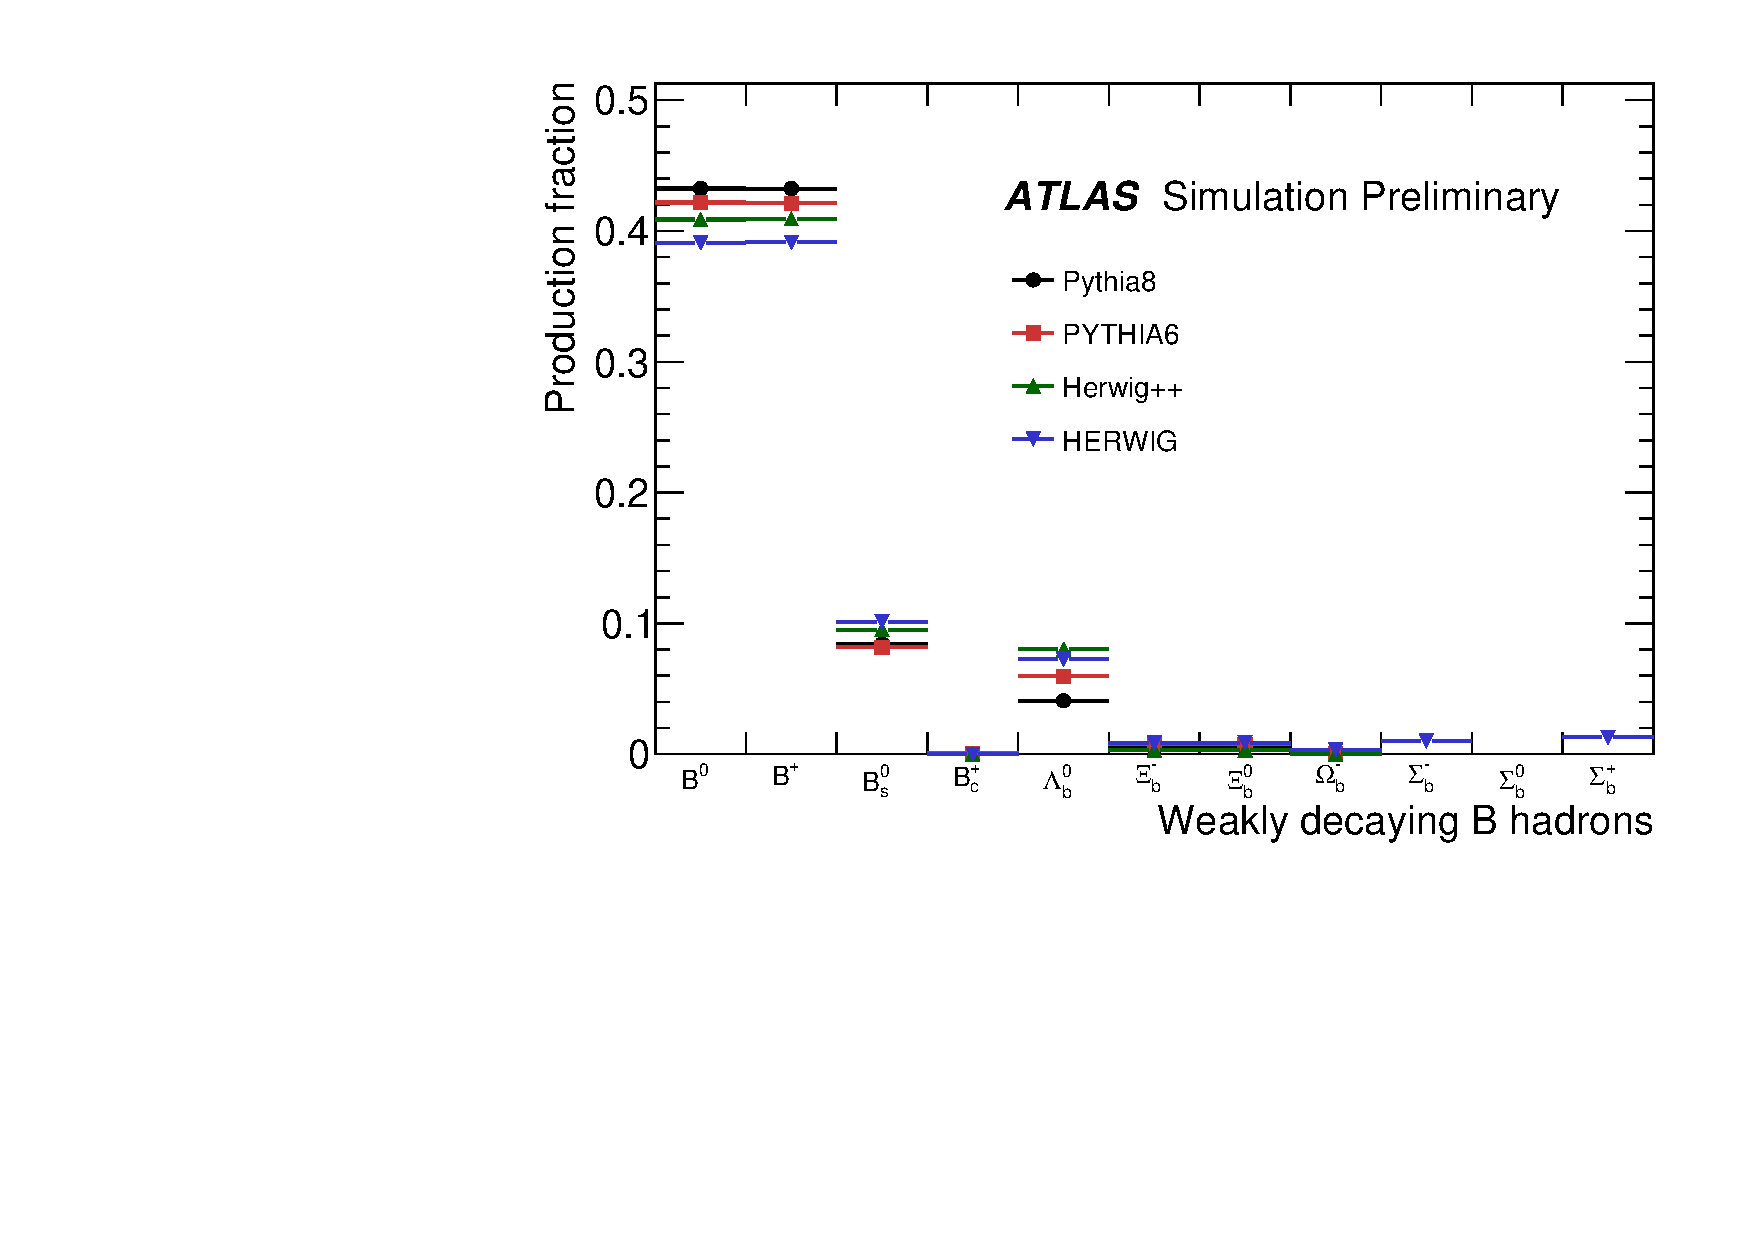
\includegraphics[width=\textwidth]{evtgen/figures/EvtGen/h_bgroundtype.pdf}
\end{subfigure}
\begin{subfigure}[]{0.5\textwidth}
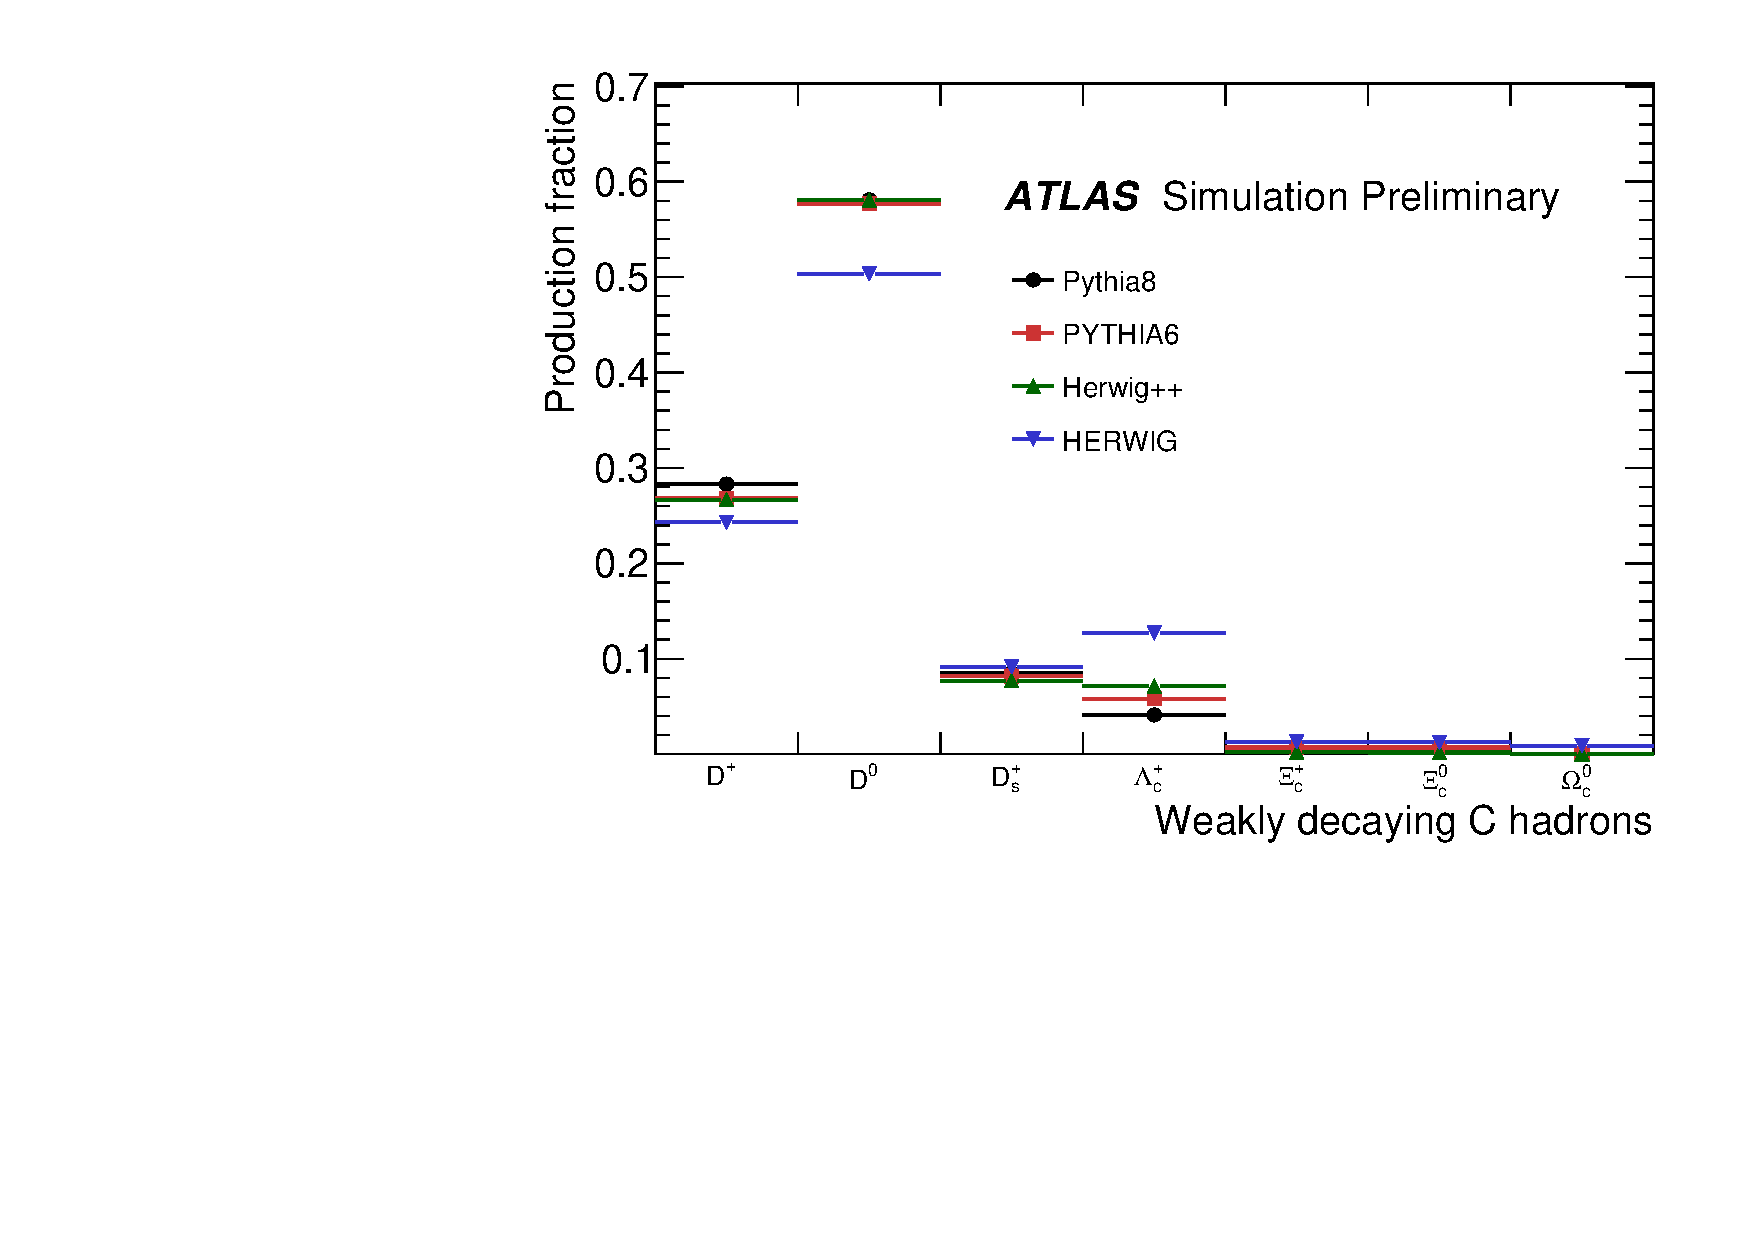
\includegraphics[width=\textwidth]{evtgen/figures/EvtGen/h_cgroundtype.pdf}
\end{subfigure}
\caption{Comparison of the production fractions for various 
weakly decaying (a) bottom and (b) charm hadrons in 
\PythiaE, \Pythia, \Herwigpp\  and \Herwig.
The $\Sigma_{b}$ should not decay weakly, but some weak decays of the $\Sigma_{b}$ are observed in 
\Herwig. 
%The generators disagree as much as 5-10\%, but the baryon fractions are not well known experimentally
}
\label{fig:prodfrac}
\end{figure}


\begin{table}
\begin{center}
\begin{tabular}{|r|r|r|r|r|r|}
\hline
Species &  \PythiaE & \Pythia & \Herwigpp & \Herwig  &  World Average\cite{PhysRevD.86.010001} \\ 
\hline 
$B^+$ &43.2 & 42.1 & 40.9 & 39.1 &   40.2 $\pm$ 0.7  \\
$B^0$  & 43.2 & 42.2 & 40.9 & 39.1 & 40.2 $\pm$ 0.7 \\
$B_s^0$ &8.4 & 8.2 & 9.5 & 10.1 &  10.4 $\pm$ 0.6\\
%$\Lambda_b^0$ & 0.0715733 & 0.0745682 & 0.0506705 & 0.0416447 & 0.08 \\
Baryons &5.1 & 7.3 & 8.6 & 11.7 &  9.3 $\pm$ 1.5\\
\hline
\end{tabular}
\caption{Percentage probability that a bottom quark decays to a bottom
hadron of a given species 
for \PythiaE, \Pythia, \Herwigpp, \Herwig\
and for the world average from Reference~\cite{PhysRevD.86.010001}.}
\label{t:bfractions}
\end{center}%
\end{table}

\begin{table}
\begin{center}
\begin{tabular}{|r|r|r|r|r|r|}
\hline
Species &  \PythiaE & \Pythia & \Herwigpp & \Herwig  & Reference~\cite{r:ffrac}\\
\hline
$D^+$ & 28.3 & 26.8 & 26.7 & 24.3 & 22.56 $\pm$ 0.77\\
$D^0$ & 58.1 & 57.7 & 58.1 & 50.3 & 56.43 $\pm$ 1.51  \\
$D_s$ & 8.5 & 8.2 & 7.7 & 9.2  & 7.97 $\pm$ 0.45\\
Baryons &5.1 & 7.2 & 7.6 & 16.2  & $10.8\pm 0.91$\\
\hline
\end{tabular}
\end{center}%
\caption{Percentage probability that a charm quark fragments to a charmed
hadron of a given species 
%for various Monte Carlo generators
for \PythiaE, \Pythia, \Herwigpp, \Herwig\
and for the world average from Reference~\cite{r:ffrac}.
%The world average baryon fraction is 
%obtained by imposing the constraint that the charm fractions add up to 1.
}
\label{t:cfractions}
\end{table}

%\section{Heavy Flavor Fragmentation}
%\label{sec:frag}
%\label{sec:fragmentation}
%
The fragmentation of a $b$- or $c$-quark into a heavy flavor hadron is modeled by the
generators using a non-perturbative fragmentation function $D_{Q}^{H}(z,\mu^2)$ that describes
the probability that a quark of species $Q$ will fragment into a hadron of species $H$ carrying
fraction $z$ of the quark's momentum~\cite{PhysRevD.86.010001}.  As with parton distribution functions, the fragmentation
functions exhibit scaling violations and therefore must be evaluated at an appropriate
scale $\mu$.  These fragmentation functions are assumed to be universal, aside from the
scale dependence, which can be calculated perturbatively. Modeling of the fragmentation functions differs among the generators, but
in all cases the parameters of the models have been tuned using data from
$e^+e^-$ collisions.  

To assess the performance of the four generators, the following strategy is used.  First,
$e^+e^-\rightarrow b\overline b$  and $e^+e^-\rightarrow c\overline c$ samples are generated 
at the center-of-mass energy of the most accurate experimental measurements, using shower parametrizations consistent with those used for the LHC tunes.
%, which have hadronization parameters tuned using both LHC and LEP data.  
These samples
are used to validate the modeling of the non-perturbative heavy flavor fragmentation functions.
Second, the evolution of fragmentation functions is studied by comparing these samples with
$e^+e^-\rightarrow b\overline b$  and $e^+e^-\rightarrow c\overline c$ events generated at
$\sqrt{s}=200$~\GeV.  Third, the fragmentation is studied for each of the
generators in the process $pp \rightarrow t \overline t$, in which the production of $b$- and $c$-jets are predominantly produced from the \ttbar\ hard scatter. Finally, to study
the case where heavy flavor is produced both in the hard scatter and in the parton
shower, samples of high \pT\ jets are analyzed.

Data on $b$-quark
fragmentation are available from LEP and SLC.  The measurements 
parametrize the fragmentation function as a function of $x \equiv E/E_{\textrm\;beam}$ where
$E$ is the energy of the bottom hadron.  Figure~\ref{fig:lepfrag}~(a) compares the distribution 

$$F(x) \equiv \frac{1}{N_{B}} \frac{dN_{B}}{dx}$$

\noindent
for the four generators to measurements from DELPHI~\cite{DELPHI}  and SLD~\cite{SLD}~. The mean values of these distributions are given in Table~\ref{t:lepfrag}.
To better match the experimental requirements on these measurements, events in the MC samples
are required to satisfy the criteria that $|\cos{\theta}_{\textrm\;thrust}|<$ 0.7 ~\footnote{The thrust axis is defined as the axis {\textbf n} that maximizes the value of${\sum\limits_{i} {\textbf n} \cdot {\textbf p_i}}/{\sum\limits_{i} {\textbf p_i} }$, where the sum is taken over all stable particles in the event.} and that
the number of weakly decaying bottom hadrons ($N_B$) satisfy $0 < N_{B}  < 3$.  The mean value of $x$
in the MC samples varies from $0.6782\pm 0.0005$ (\Herwig) to $0.7303\pm 0.0005$ (\PythiaE).
\Pythia\ and \Herwigpp\ agree well with the data, while \PythiaE\ is high by $\sim 2\%$ and
\Herwig\ is low by $\sim 3\%$.  These results are consistent with those presented in Reference~\cite{Karneyeu:2013aha}.

Figure~\ref{fig:lepfrag}~(b) shows the same distribution
for the four generators at a center-of-mass energy of $\sqrt{s}=200$~GeV.  The samples are generated without initial state QED in order to isolate the effect of increased $\sqrt{s}$.  As expected,
the mean value of $x$ is lower than at the $Z$-pole, due the evolution of the
fragmentation function.  The ratio of the means at the higher energy to those at the 
lower energy are 93.8\%, 95.8\%, 94.0\%\ and 97.2\% for \PythiaE, \Pythia, \Herwigpp\ and \Herwig\ 
respectively.

Studies of $c$-quark fragmentation are available from Belle~\cite{Belle} and CLEO~\cite{CLEO}. 
The fragmentation function is measured as a function of $x_p \equiv p/p_{\textrm\;max}$ where
$p$ is the momentum of the charm hadron and $p_{\textrm\;max}$ is the maximum momentum that
is kinematically allowed.  Charm hadrons are required to be directly produced; bottom hadron decay products are
excluded.
Figures~\ref{fig:belle}~(a) and ~\ref{fig:belle}~(b) compare the four generators to the experimental measurements for $D^+$ and
$D^0$ mesons respectively. Table~\ref{t:belle}~ gives the mean value of the fragmentation functions. The \PythiaE\ fragmentation appears to be significantly harder than the data, while 
other generators agree reasonably well with the data and with each other.
%n hadron collisions...sentence changed. I THINK physics is right...

In $e^+e^-$ collisions, the fragmentation function can be measured relative to the beam energy, since the 
momentum transfer of the hard scatter is fixed by the energy of the initial beams (aside from initial state photon radiation). However, fragmentation in hadron collisions must be parameterized with respect to the output of a jet-finding algorithm. By convention, the \pT\ of the jet containing the
heavy flavor hadron is used to approximate the unknown \pT\ of the heavy flavor parton.
The resulting fragmentation function $f(z)$ is defined to be

$$
f(z) \equiv \frac{\vec{p}_{\textrm\;hadron} \cdot \vec{p}_{\textrm\;jet} } {{p^2}_{\textrm\;jet}}.
$$
\noindent

For this study, the $f(z)$ is measured for \antiktfour\ jets with $|\eta^{\textrm\;jet}| < 2.5$.  Jets are defined
to be heavy flavor jets if there is a weakly decaying heavy flavor hadron with $\pt>5$\,\GeV\ 
%with transverse momentum $\pt>25$\,\GeV\ 
%containing a weakly decaying heavy flavor hadron with $\pt>5$\,\GeV\ 
within $\Delta R=\sqrt{\Delta \phi^2 +\Delta \eta^2}<0.3$ of the jet direction.
For measurements of the charm fragmentation function, jets are vetoed if the charm
hadron contained in the jet is a bottom hadron decay product. 

 For large momentum scale processes,
an additional perturbative contribution (from $g\rightarrow b \overline b$) becomes significant. 
In some cases, this perturbative component is explicitly included in
the matrix element calculation, while in other cases this component is treated as part
of the parton shower. Such jets are included here in the definition of $b$- and $c$- jets.

Figure~\ref{fig:tfrag} and Table~\ref{t:tfrag} show the  bottom and  charm fragmentation functions $f(z)$ for  
jets in the \ttbar\ samples satisfying the requirement \ptJet\ \textgreater~25~\GeV\ 
in events containing a lepton with $p_T^{\textrm\;lep} > 20$ GeV and $|\eta^{\textrm\;lep}| < 2.5$. The mean value of $z$ varies from 0.741 (\Herwig) to 0.772 (\Herwigpp) for $b$-quarks
and from 0.552 (\Pythia) to 0.575 (\Herwig) for $c$-quarks.  The $b$-quark ($c$-quark) fragmentation in 
\Herwigpp\ (\Herwig) is noticeably harder than for the other generators.

The fragmentation function in jets is sensitive to many other aspects of the simulation. Measurements
depend on the choice of jet algorithm and can be affected by the underlying event tune, as well as by the
transverse shape of the generated jet.  Details of the shower modeling itself, such as the suppression of 
QCD radiation from heavy particles (the \textit{dead-cone} effect~\cite{Marchesini:1989yk}) can also play a role.
%Such effects can result in differences for the lighter charm and the heavier bottom.
To better study the fragmentation model, these effects are probed using additional distributions
for these heavy flavor jets.  Figure~\ref{fig:twidth} shows the width of the 
$b$-quark and  $c$-quark jets, where the jet width ($W$) is obtained from the \pT\ weighted
distribution of the distance $\Delta R$ from the center of the jet: 

$$
W \equiv \frac{\sum_{i} {p_{T}}_i \; \Delta R_{i}}{\sum_{i} {p_{T}}_i}
$$
\noindent
and the sum is taken over all stable particles that are constituents of the jets.    The mean value
of the jet widths for all generators agree to within a few percent, although the distribution of
widths for $b$-quark jets is slightly broader for \PythiaE\ than for the other generators and the
distribution of widths for $c$-quarks is slightly narrower for \Herwig\ and \Herwigpp\
than for \Pythia\ and \PythiaE.

\begin{figure}
\centering
\begin{subfigure}[]{0.45\textwidth}
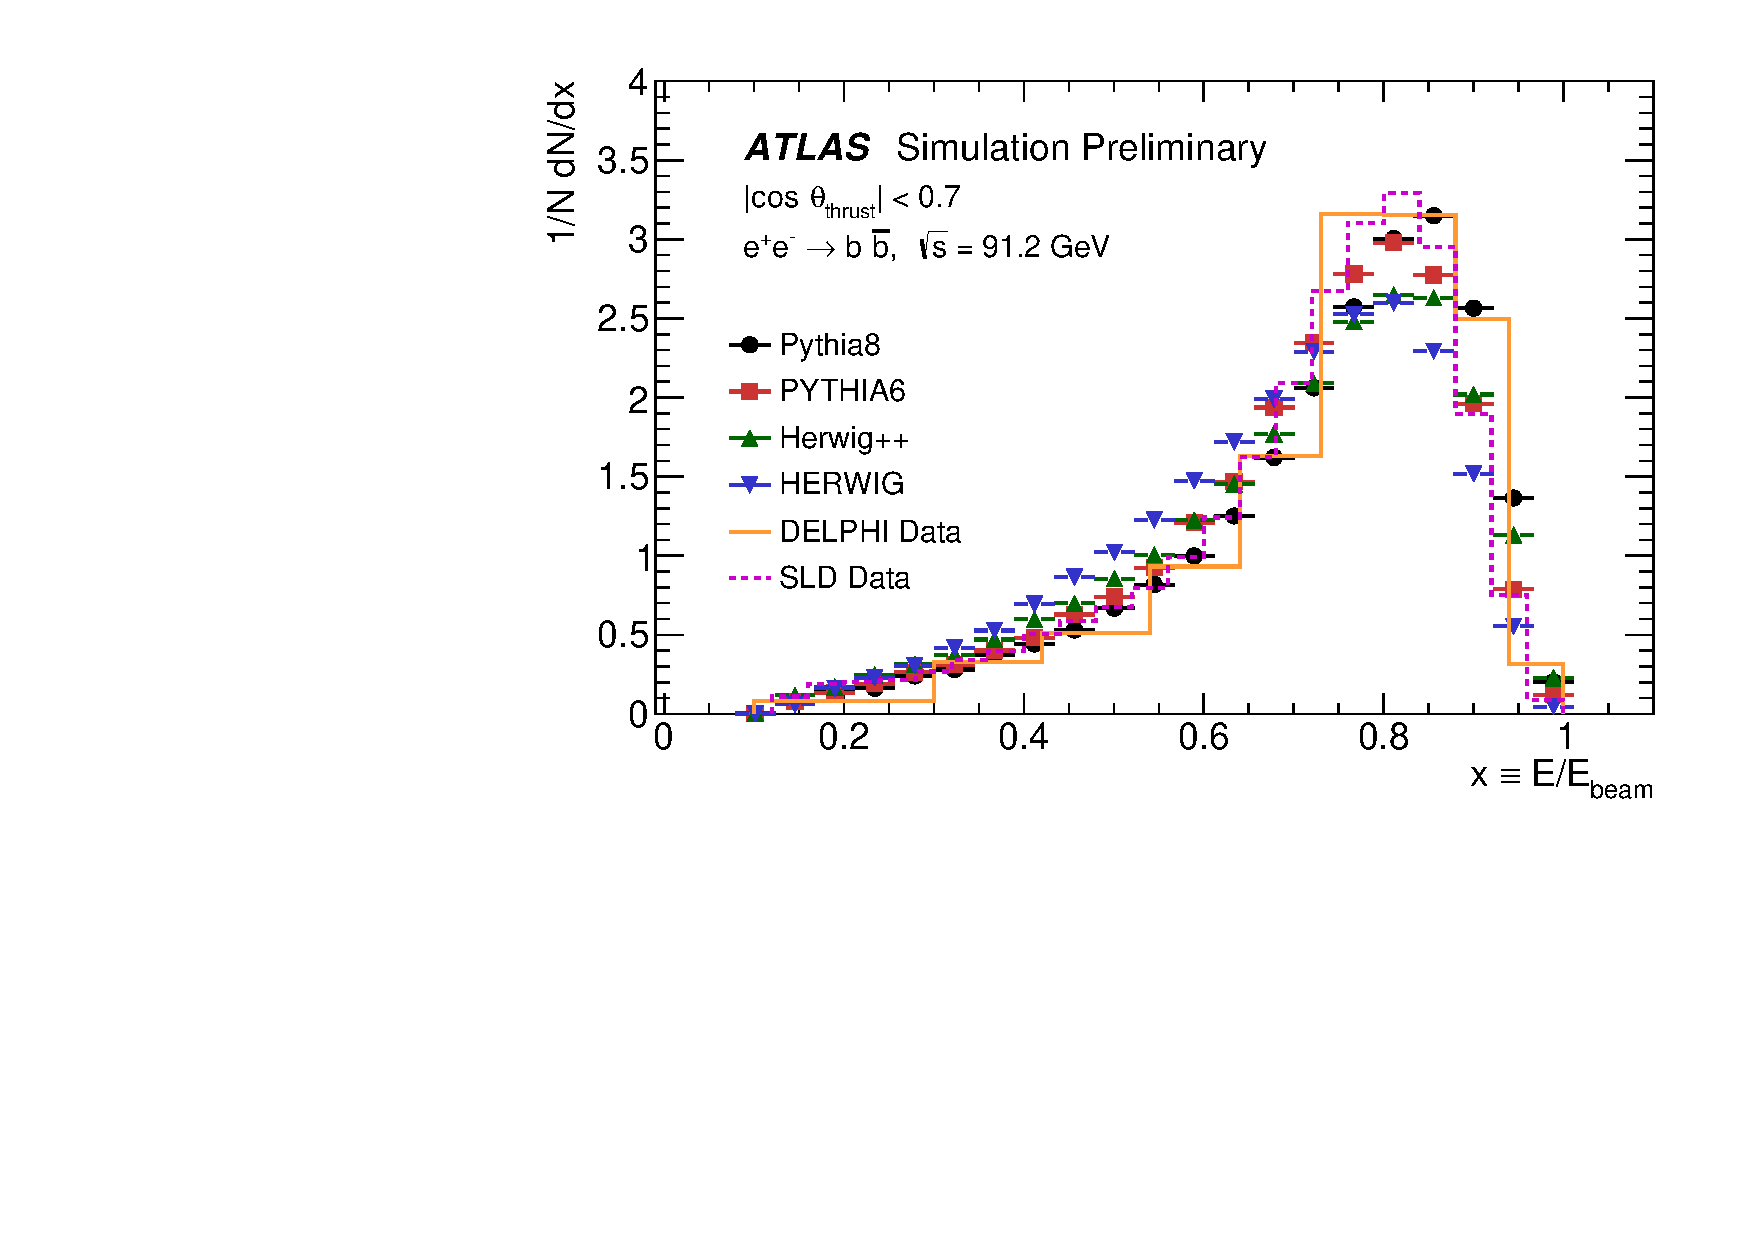
\includegraphics[width=\textwidth]{evtgen/figures/Frag/LEP.pdf}
\end{subfigure}
\begin{subfigure}[]{0.45\textwidth}
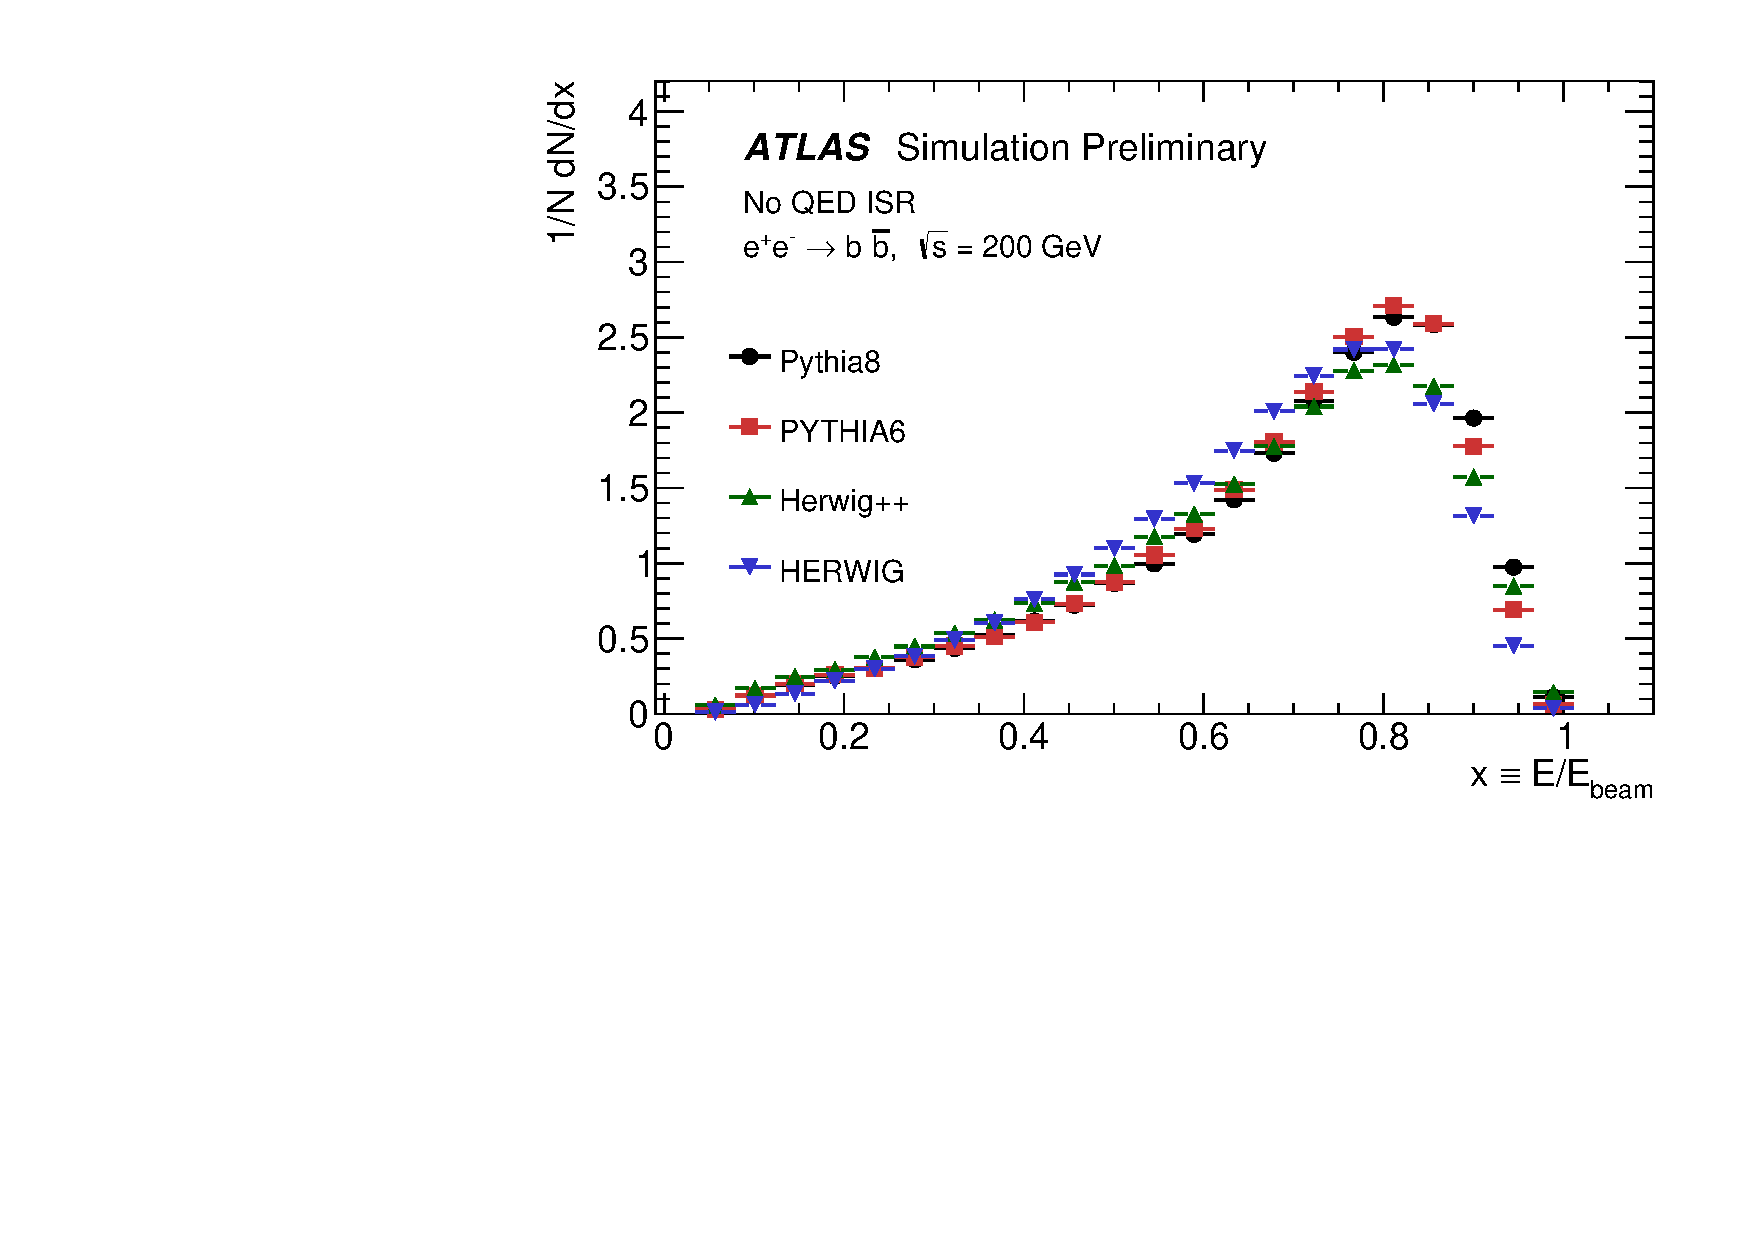
\includegraphics[width=\textwidth]{evtgen/figures/Frag/200GeV/h_Xweak_B.pdf}
\end{subfigure}
\caption{The $b$-quark fragmentation function obtained 
with \PythiaE, \Pythia, \Herwigpp\ and \Herwig\  
for (a)~$\sqrt{s}=91.2$~\GeV\ and (b)~$\sqrt{s}=200$~\GeV\ $e+e-$ collisions. 
DELPHI and SLD data in (a) are taken from References~\cite{DELPHI} and~\cite{SLD} respectively and are plotted without error bars.  }
\label{fig:lepfrag}
\end{figure}


\begin{table}
\begin{center}
\begin{tabular}{|r|r|}
\hline
\multicolumn{2}{|c|}{$E_{B}/E_{beam}$} \\
\hline
\hline
 \PythiaE & $0.7303 \pm 0.0005$ \\
 \Pythia & $0.7090 \pm 0.0005$ \\
 \Herwigpp & $0.7012 \pm 0.0006$ \\
 \Herwig  & $0.6782 \pm 0.0005$ \\
\hline
 Delphi Data & $0.699 \pm 0.011$ \\
 SLD Data & $0.709 \pm 0.005$ \\
\hline 

\hline
\end{tabular}
\caption{The mean $b$-quark fragmentation function obtained 
with \PythiaE, \Pythia, \Herwigpp\ and \Herwig\  
for $\sqrt{s}=91.2$~\GeV\ in $e+e-$ collisions. 
DELPHI and SLD data in (a) are taken from References~\cite{DELPHI} and~\cite{SLD} respectively.}
\label{t:lepfrag}
\end{center}%
\end{table}

\begin{figure}
\centering
 \begin{subfigure}[]{0.45\textwidth}
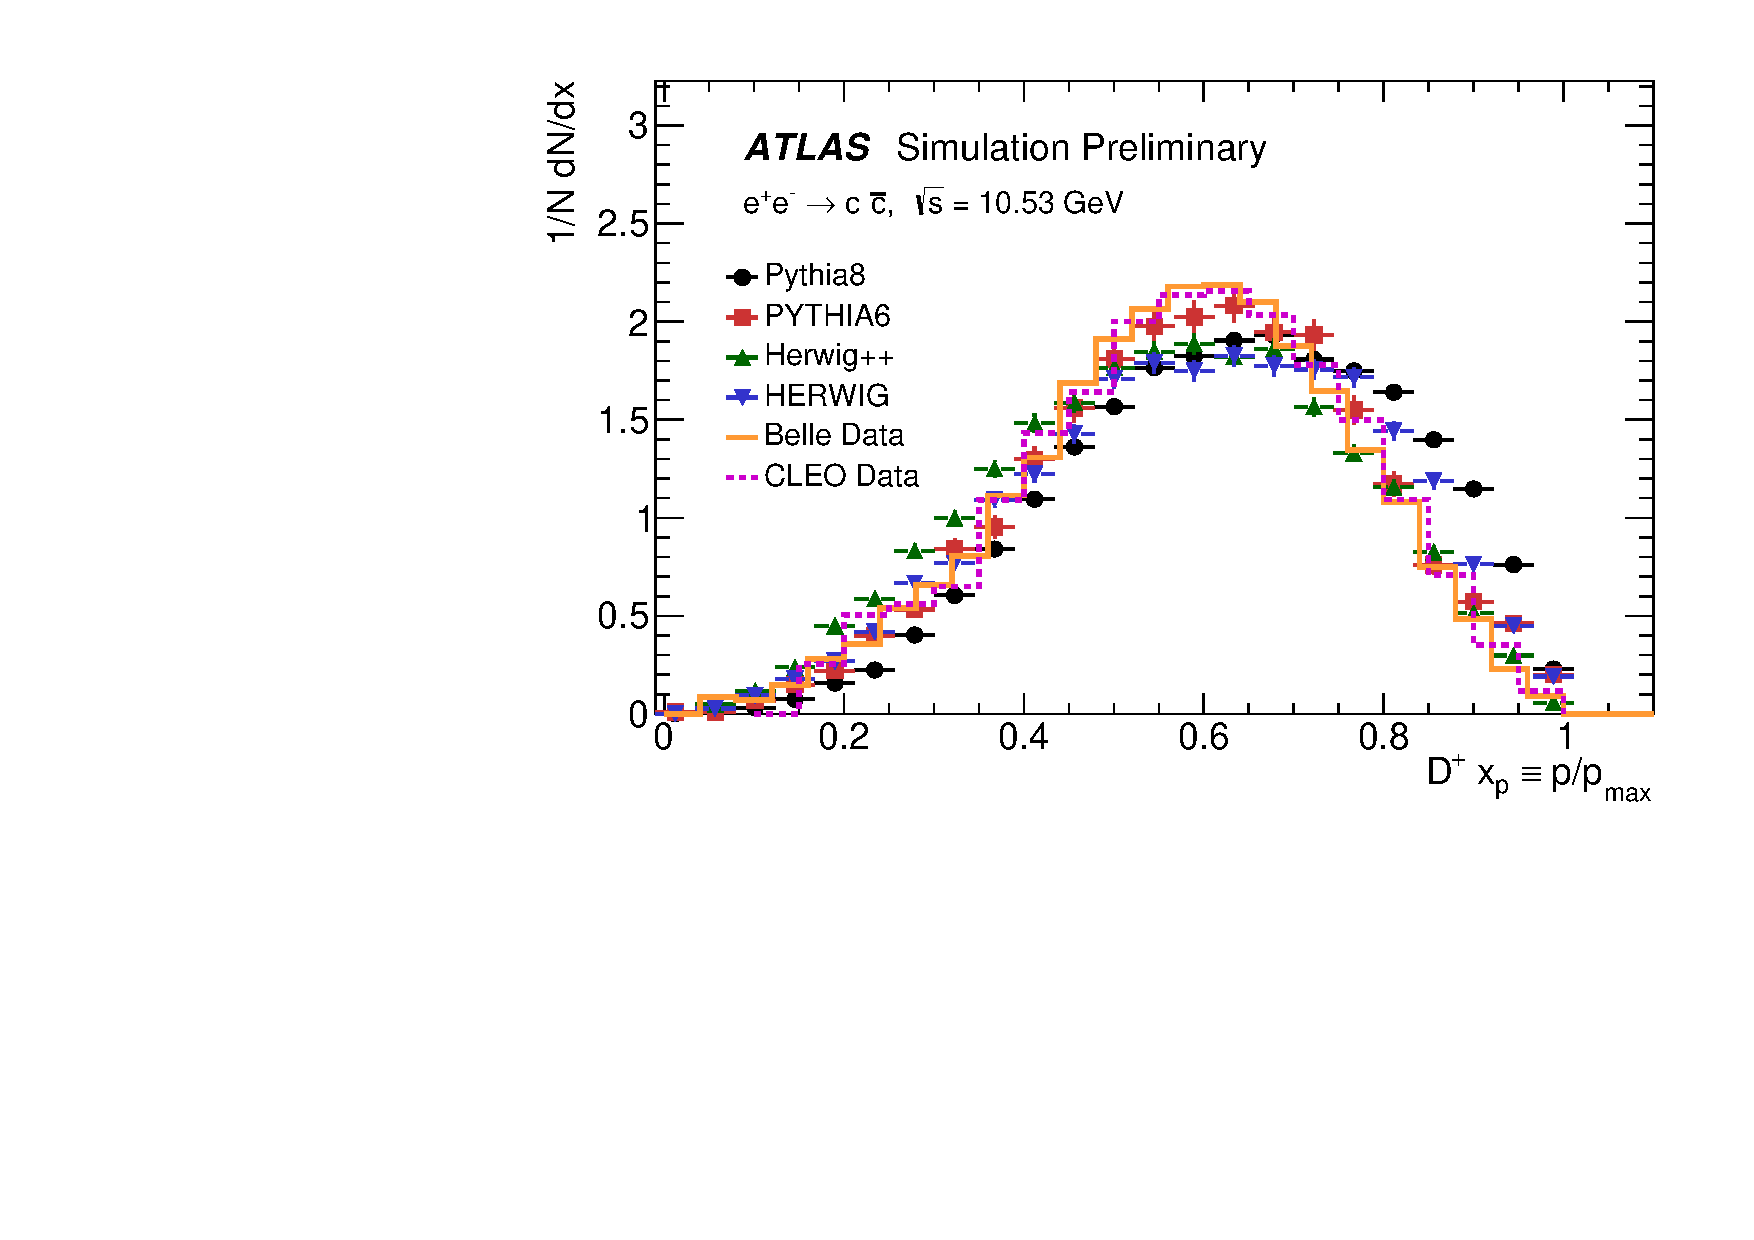
\includegraphics[width=\textwidth]{evtgen/figures/Frag/DPlusFrag.pdf}
\end{subfigure}
 \begin{subfigure}[]{0.45\textwidth}
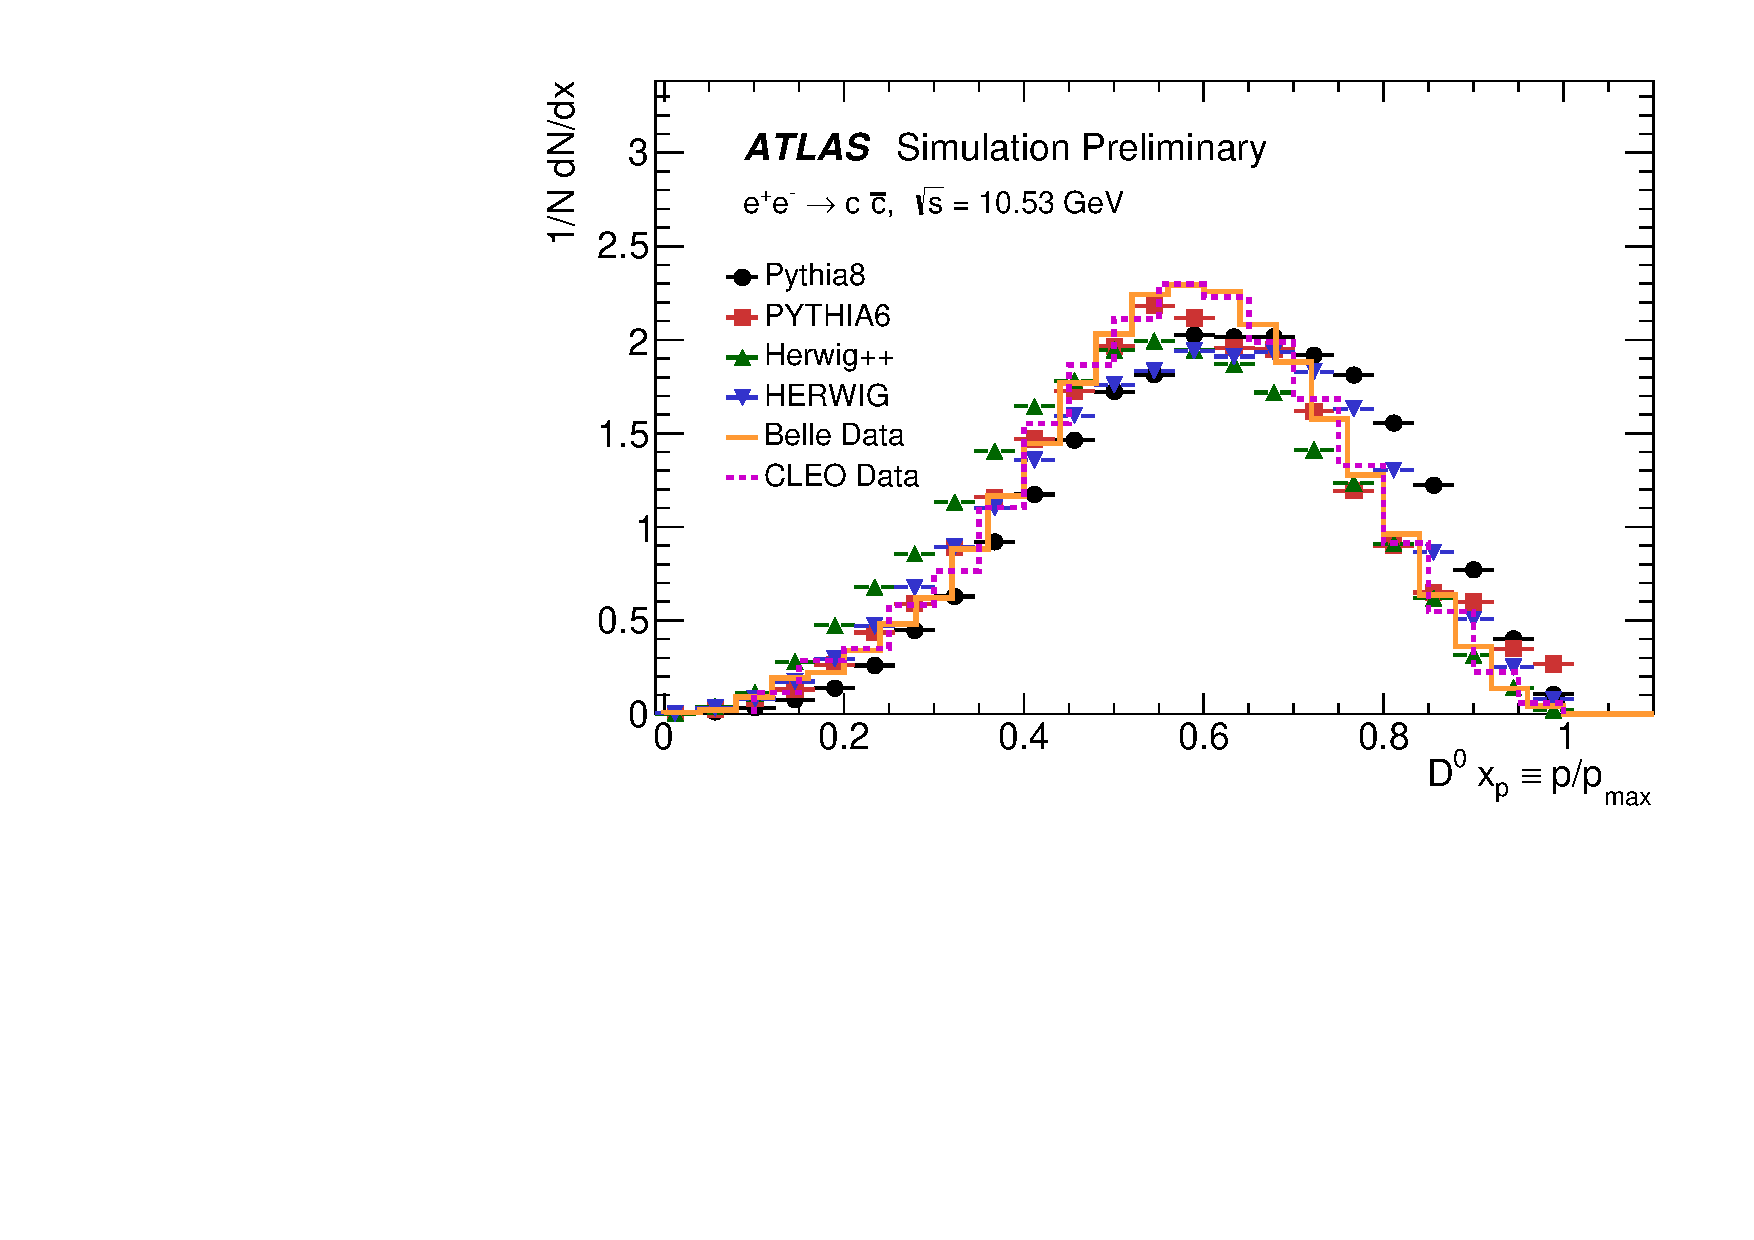
\includegraphics[width=\textwidth]{evtgen/figures/Frag/D0Frag.pdf}
\end{subfigure}
\begin{subfigure}[]{0.45\textwidth}
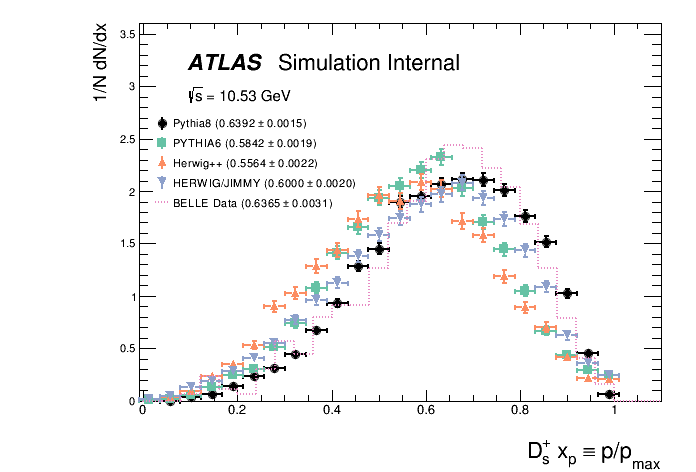
\includegraphics[width=\textwidth]{evtgen/figures/Frag/DSplusFrag.pdf}
\end{subfigure}
\caption{The $c$-quark fragmentation function obtained 
with \PythiaE, \Pythia, \Herwigpp\ and \Herwig\  
for $\sqrt{s}=10.53$~\GeV\ for $e+e-$ collisions for
(a)~$D^+$ and (b)~$D^0$ mesons. CLEO and Belle data are taken from References~\cite{CLEO} and~\cite{Belle}
respectively and are plotted without error bars. }
\label{fig:belle}
\end{figure}

\begin{table}
\begin{center}
\begin{tabular}{|r|r|r|}
\hline
\multicolumn{3}{|c|}{$p_{C}/p_{max}$} \\
\hline
& $D^+$ & $D^0$ \\
\hline
\hline
 \PythiaE & $0.6337 \pm 0.0010$ & $0.6156 \pm 0.0007$ \\
 \Pythia & $0.5918 \pm 0.0022$ & $0.5744 \pm 0.0011$ \\
 \Herwigpp & $0.5611 \pm 0.0016$ & $0.5390 \pm 0.0010$ \\
 \Herwig  & $0.5981 \pm 0.0016$ & $0.5797 \pm 0.0011$ \\
\hline
 Belle Data & $0.578 \pm 0.00148$ & $0.5703 \pm 0.0020$ \\
CLEO Data & $0.582 \pm 0.009$ & $0.570 \pm 0.006$ \\
\hline 

\hline
\end{tabular}
\caption{The mean $c$-quark fragmentation function obtained 
with \PythiaE, \Pythia, \Herwigpp\ and \Herwig\  
for $\sqrt{s}=10.53$~\GeV\ for $e+e-$ collisions for
(a)~$D^+$ and (b)~$D^0$ mesons. CLEO and Belle data are taken from References~\cite{CLEO} and~\cite{Belle}
respectively.}
\label{t:belle}
\end{center}%
\end{table}


\begin{figure}
\centering
\begin{subfigure}[]{0.45\textwidth}
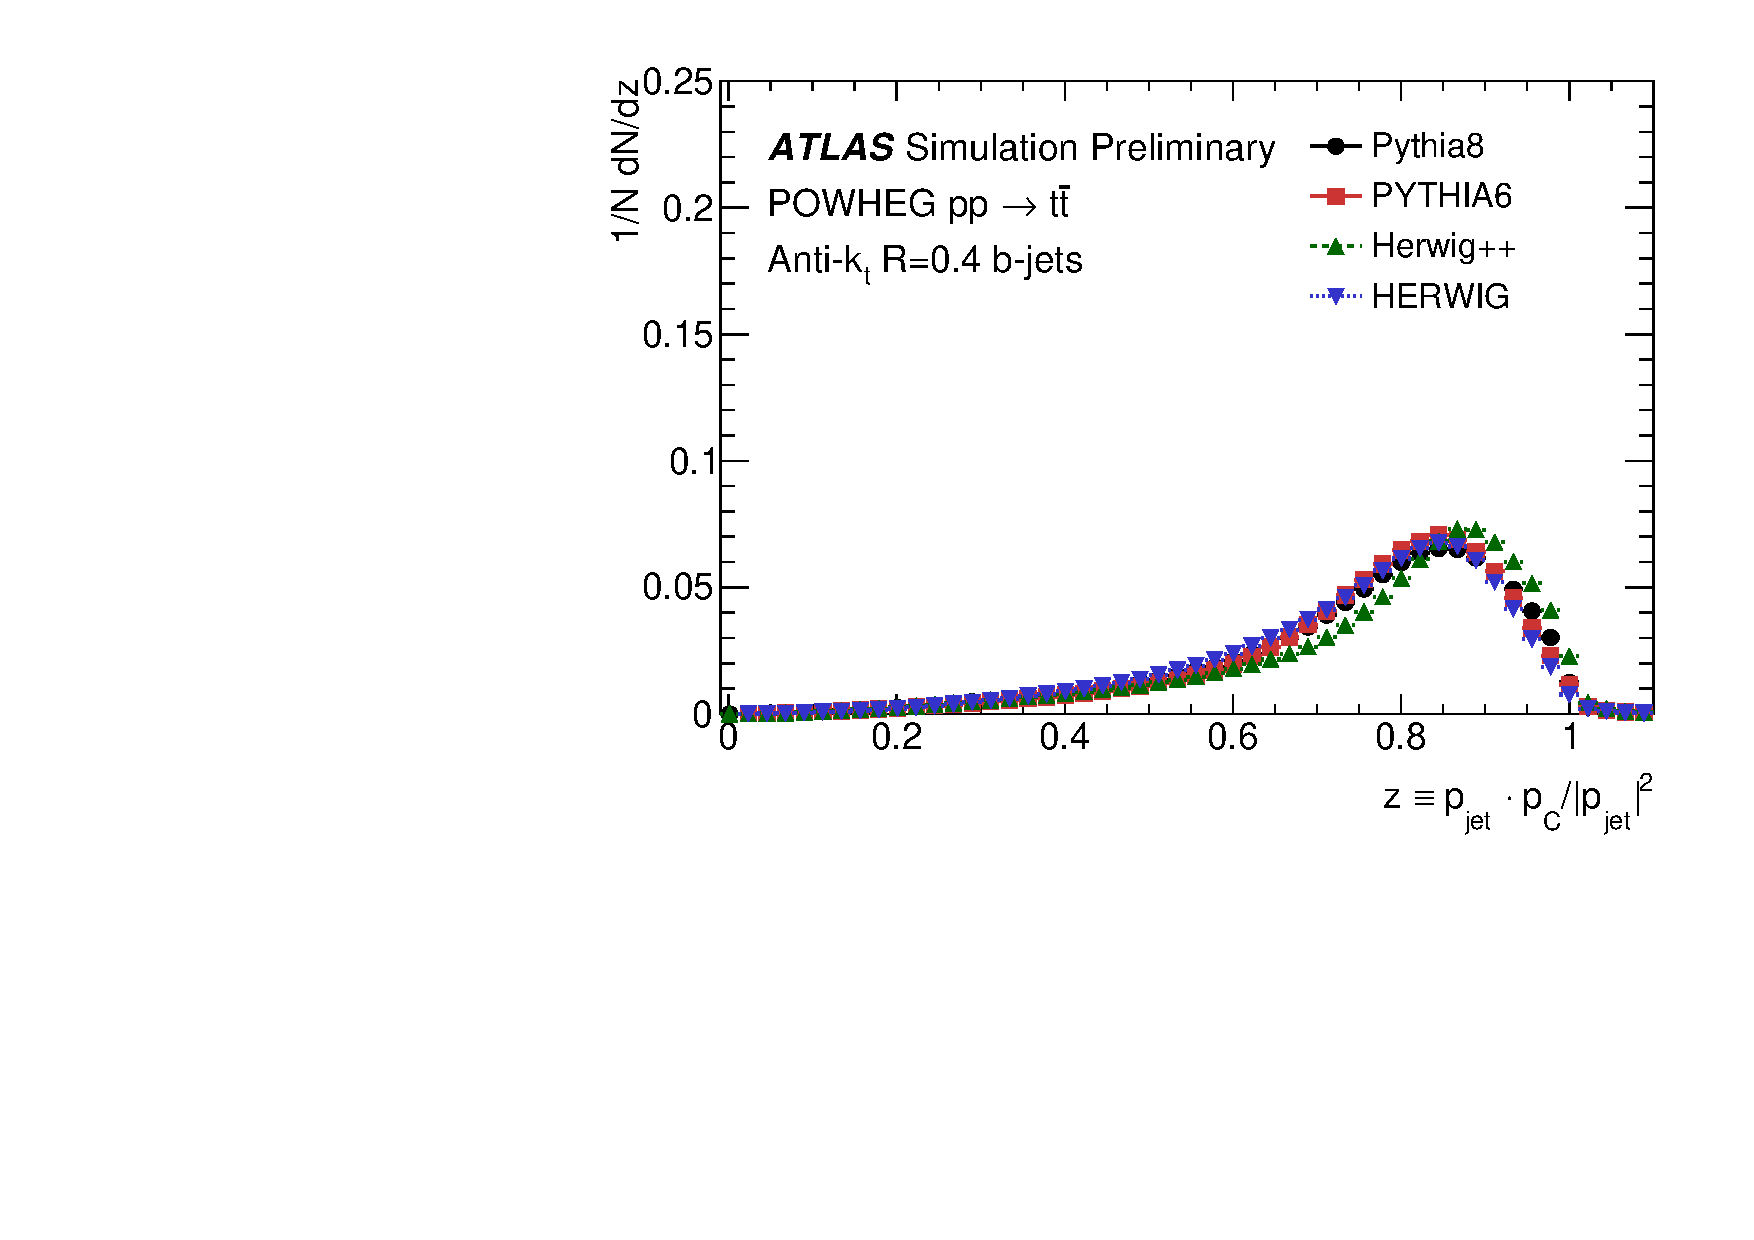
\includegraphics[width=\textwidth]{evtgen/figures/Frag/Top/h_BFrag_SingleHad.pdf}
\end{subfigure}
\begin{subfigure}[]{0.45\textwidth}
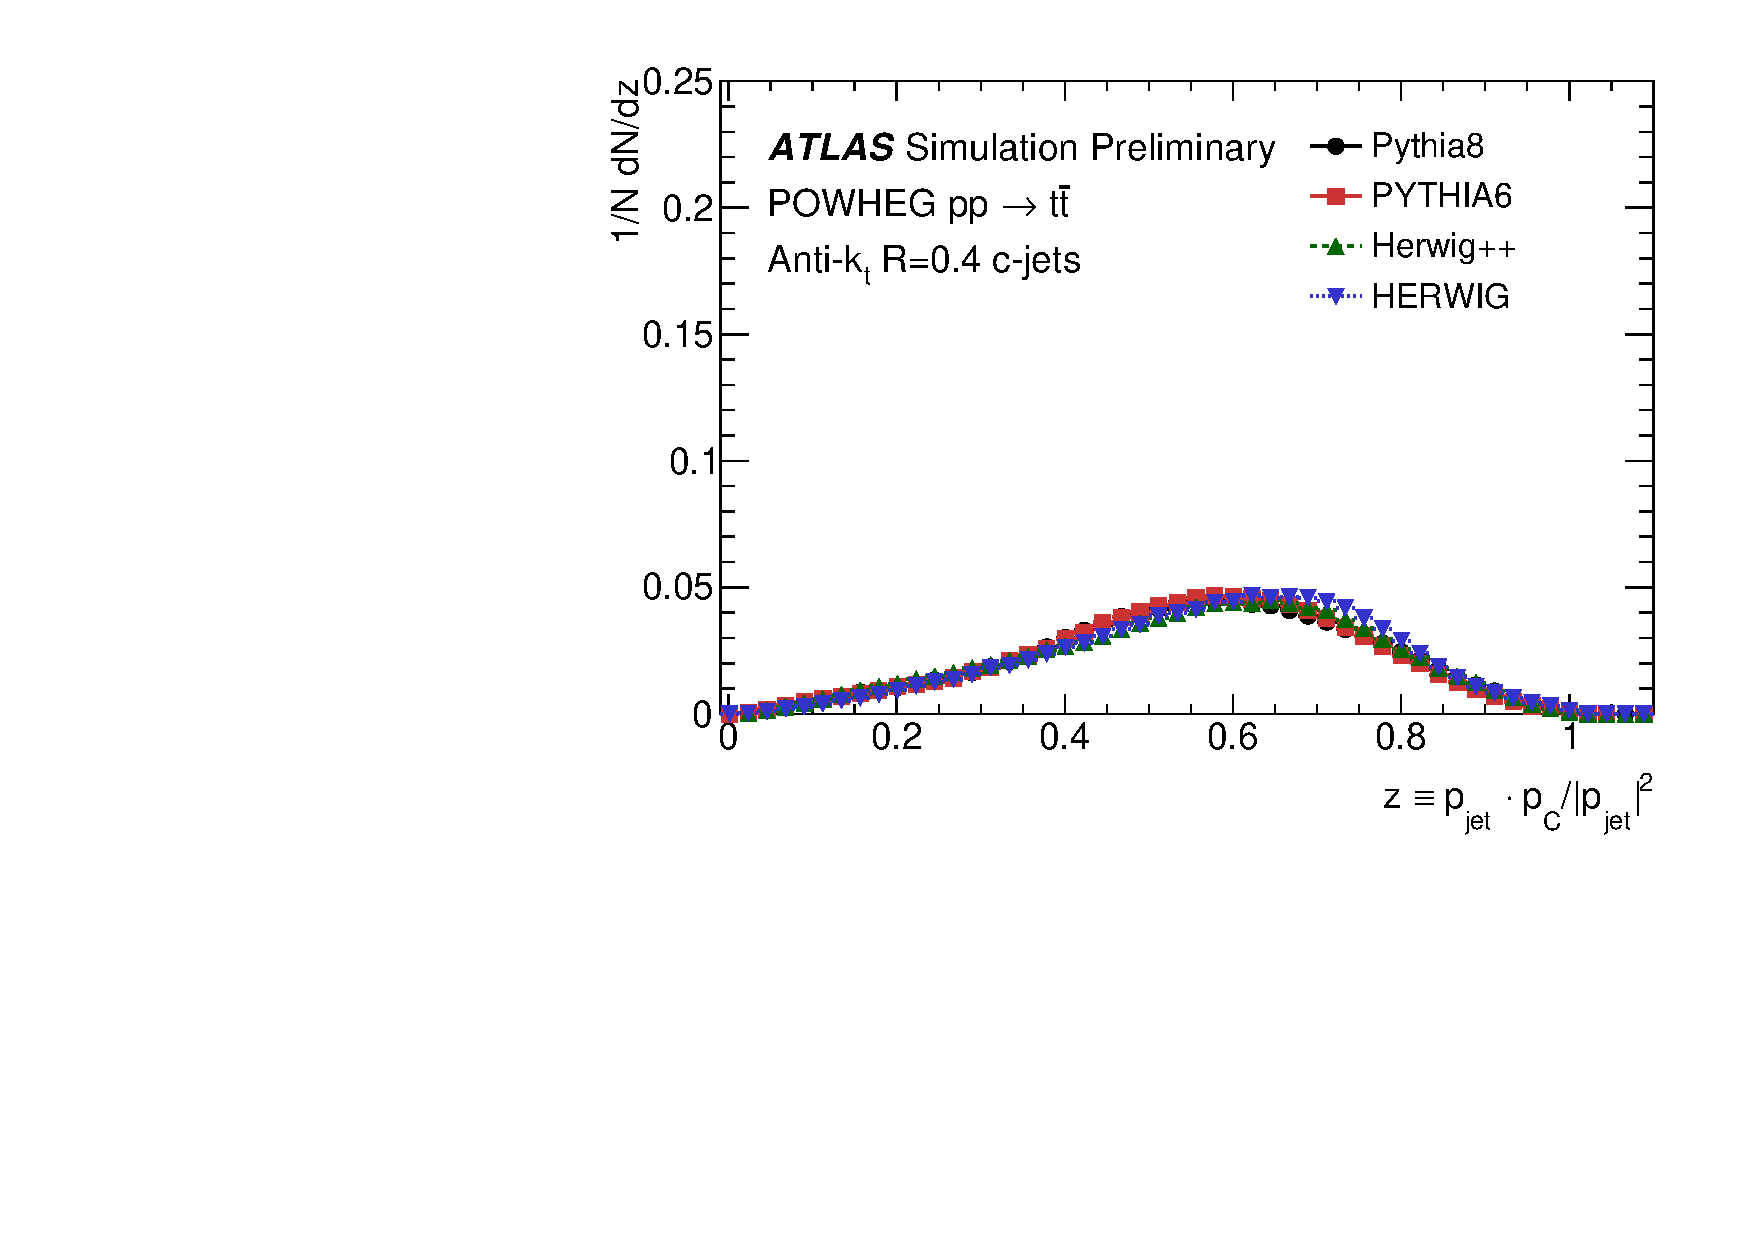
\includegraphics[width=\textwidth]{evtgen/figures/Frag/Top/h_CFrag_SingleHad.pdf}
\end{subfigure}
\caption{The fragmentation function for 
%(a)~$b$-jets and (b)~$c$-jets in \PowHeg\
%\ttbar\ samples where  \PythiaE, \Pythia, \Herwigpp\ and \Herwig\ have been used 
for the parton shower, hadronization and underlying event modeling.}
\label{fig:tfrag}
\end{figure}

\begin{table}
\begin{center}
\begin{tabular}{|r|r|r|}
\hline
Generator & $p_{jet} \cdot p_{B}/p_{jet}^2$  & $p_{jet} \cdot p_{C}/p_{jet}^2$ \\
\hline
 \PythiaE & $0.7529 \pm 0.0001$ & $0.5550 \pm 0.0004$  \\
 \Pythia & $0.7561 \pm 0.0001$  & $0.5525 \pm 0.0004$  \\
 \Herwigpp & $0.7719 \pm 0.0001$   & $0.5590 \pm 0.0004$  \\
 \Herwig  & $0.7411 \pm 0.0001$  & $0.5751 \pm 0.0004$  \\

\hline
\end{tabular}
\caption{The mean fragmentation function for 
$b$-jets and  $c$-jets in \PowHeg\
\ttbar\ samples where  \PythiaE, \Pythia, \Herwigpp\ and \Herwig\ have been used 
for the parton shower, hadronization and underlying event modeling.}
\label{t:tfrag}
\end{center}%
\end{table}

\begin{figure}
\centering
\begin{subfigure}[]{0.45\textwidth}
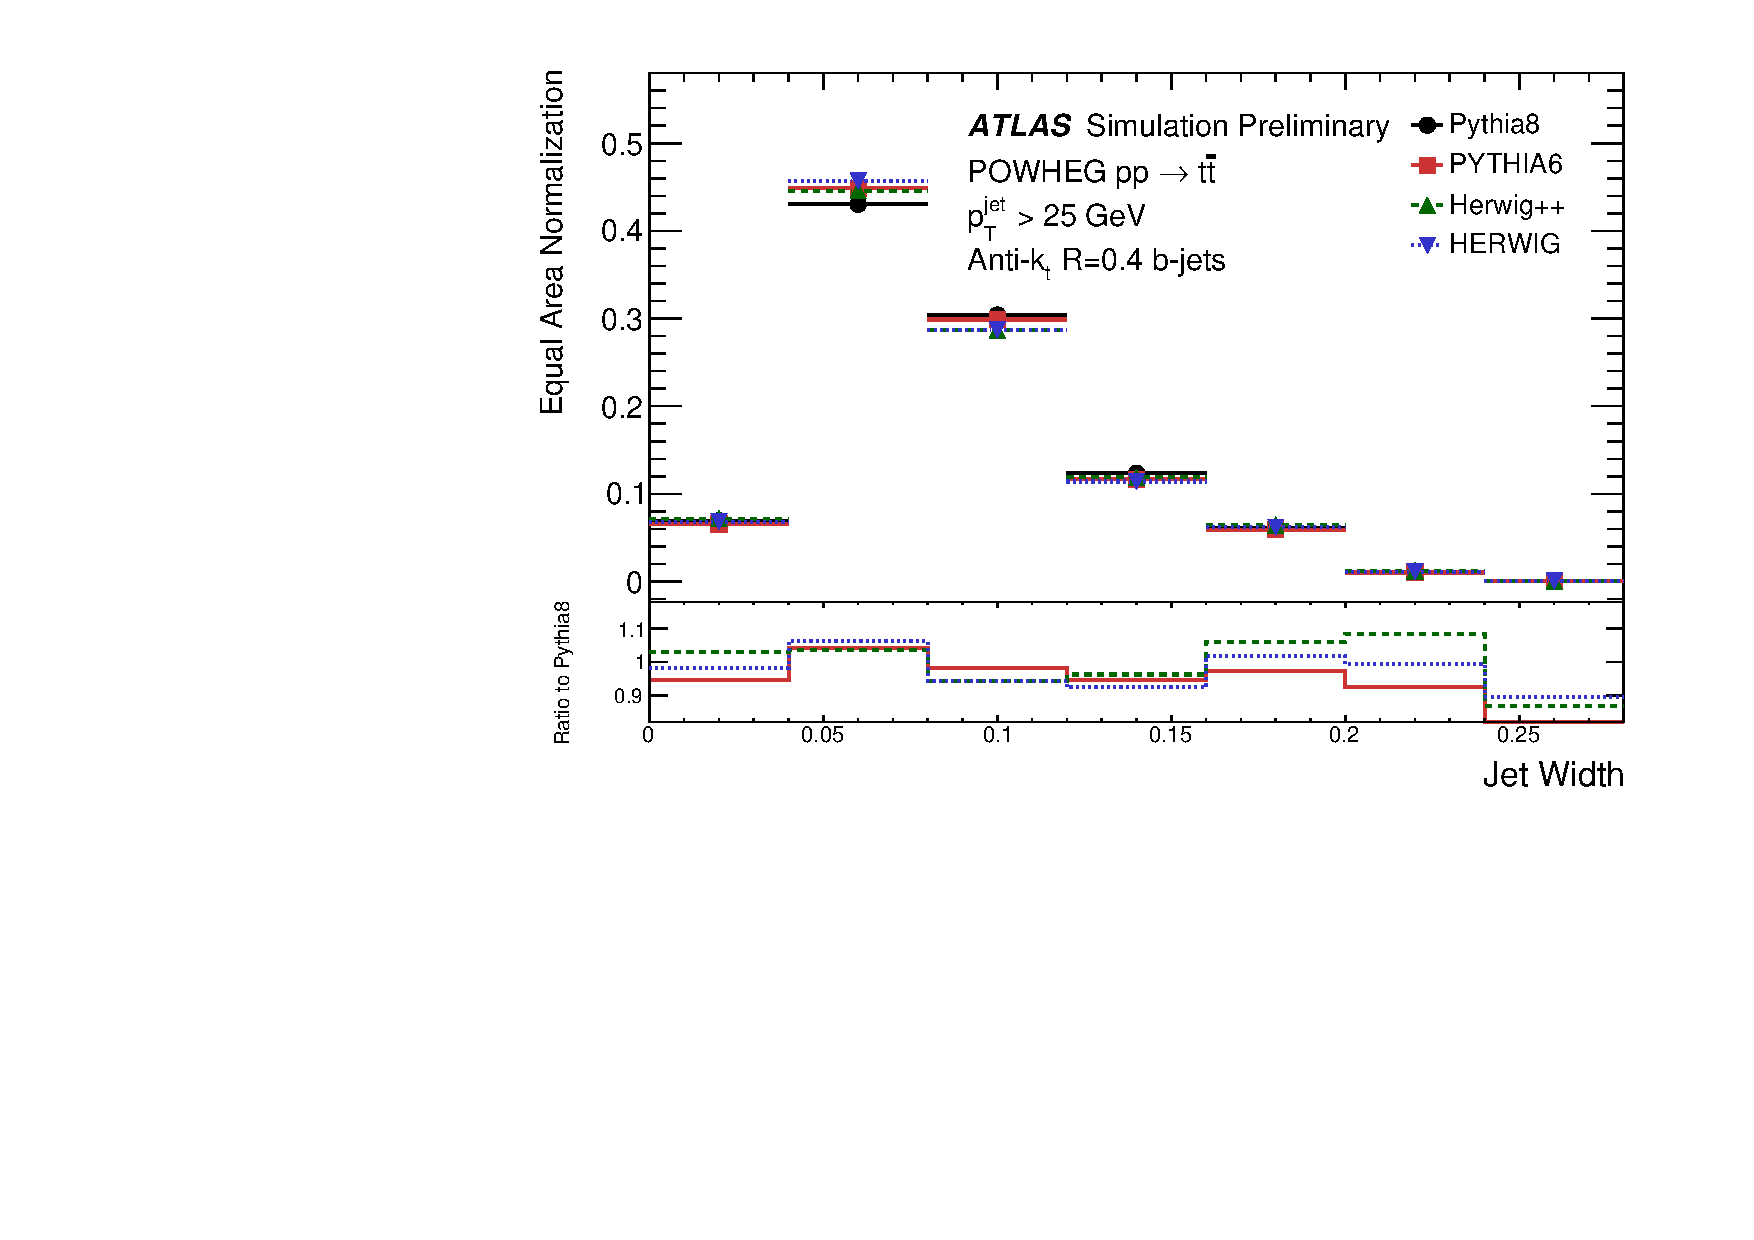
\includegraphics[width=\textwidth]{evtgen/figures/Frag/Top/SingleB/h_JetWidth.pdf}
\end{subfigure}
\begin{subfigure}[]{0.45\textwidth}
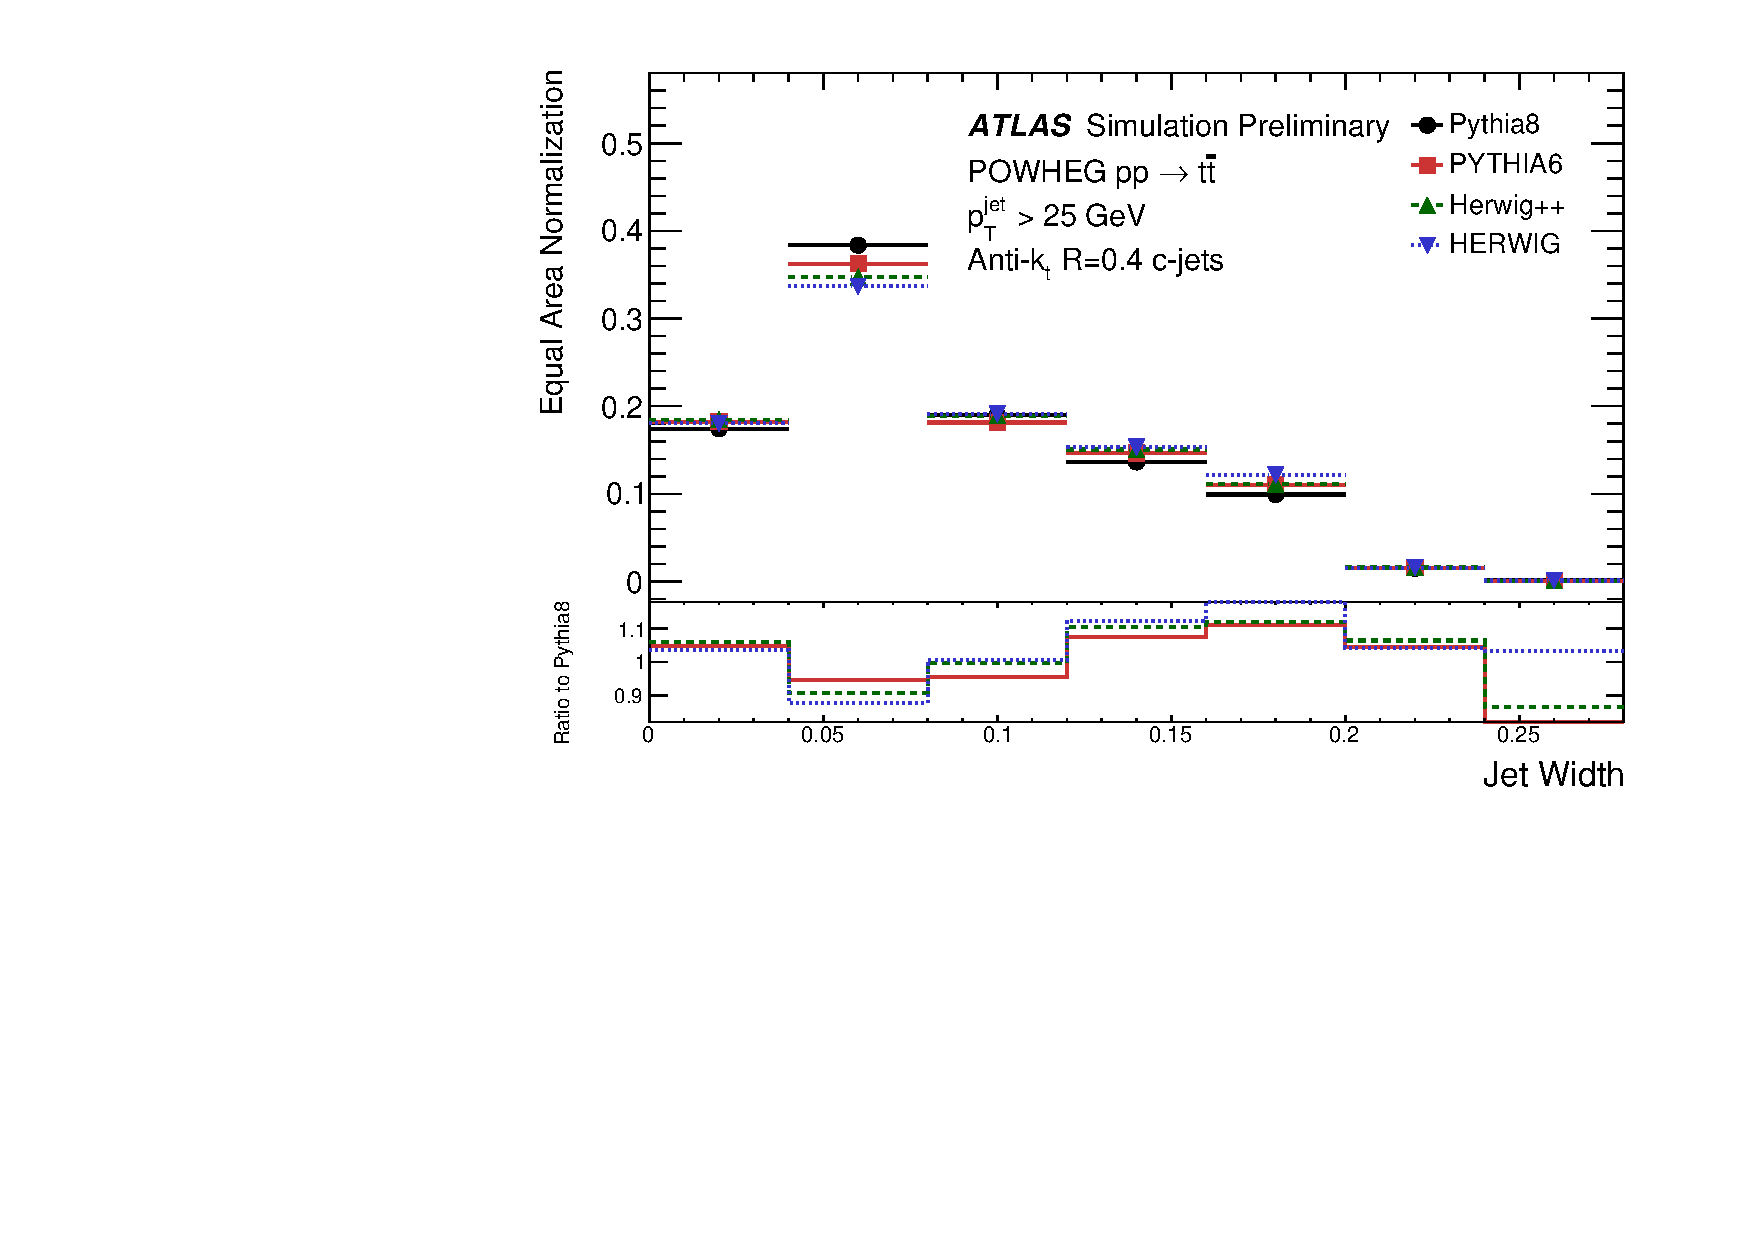
\includegraphics[width=\textwidth]{evtgen/figures/Frag/Top/SingleC/h_JetWidth.pdf}
\end{subfigure}
\caption{The jet width for 
(a)~$b$-jets and (b)~$c$-jets in \PowHeg\
\ttbar\ samples where  \PythiaE, \Pythia, \Herwigpp\ and \Herwig\ have been used 
for the parton shower, hadronization and underlying event modeling. }
\label{fig:twidth}
\end{figure}

\begin{figure}
\centering
\begin{subfigure}[]{0.45\textwidth}
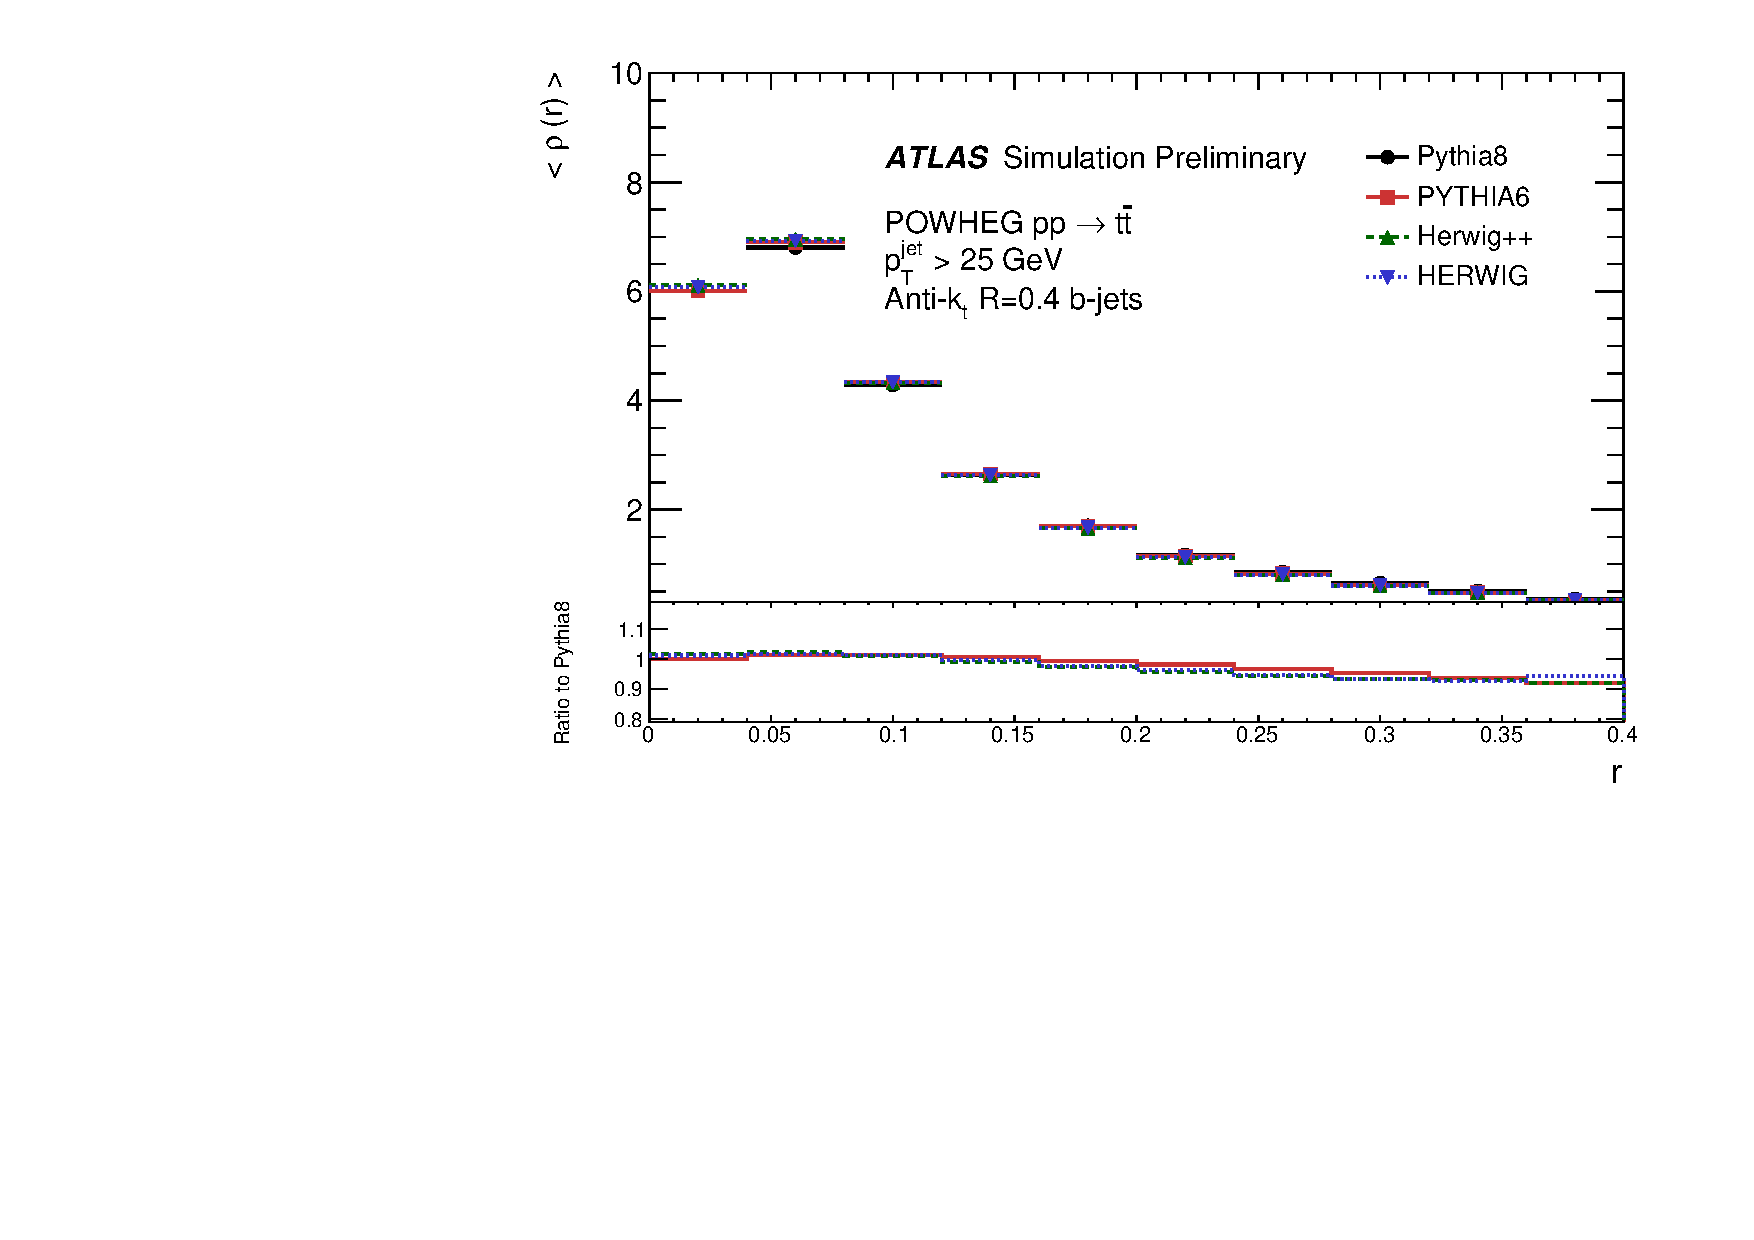
\includegraphics[width=\textwidth]{evtgen/figures/Frag/Top/SingleB/Rho.pdf}
\end{subfigure}
\begin{subfigure}[]{0.45\textwidth}
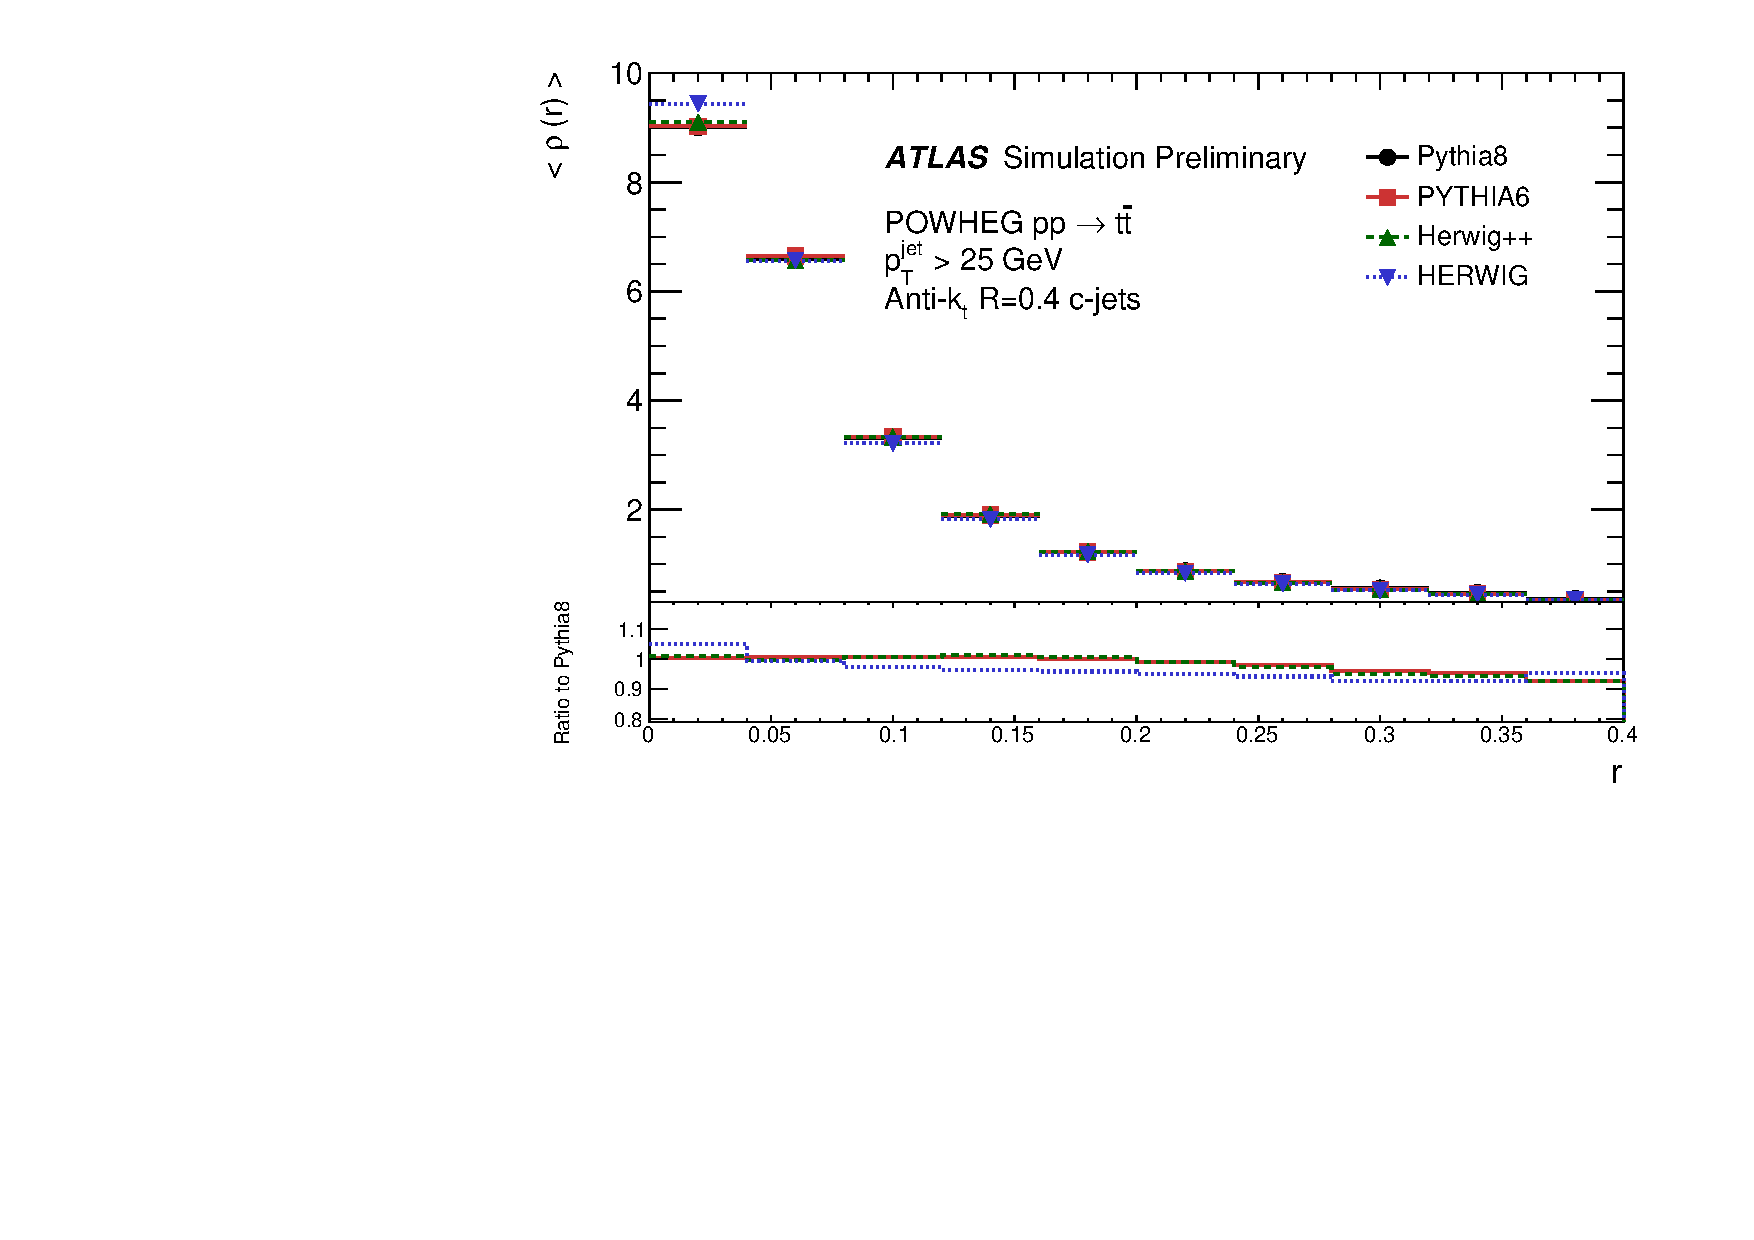
\includegraphics[width=\textwidth]{evtgen/figures/Frag/Top/SingleC/Rho.pdf}
\end{subfigure}
\caption{The differential jet shape $\rho(r)$ distribution for 
(a)~$b$-jets and (b)~$c$-jets in \PowHeg\
\ttbar\ samples where  \PythiaE, \Pythia, \Herwigpp\ and \Herwig\ have been used 
for the parton shower, hadronization and underlying event modeling. }
\label{fig:trho}
\end{figure}


\begin{figure}
\centering
\begin{subfigure}[]{0.45\textwidth}
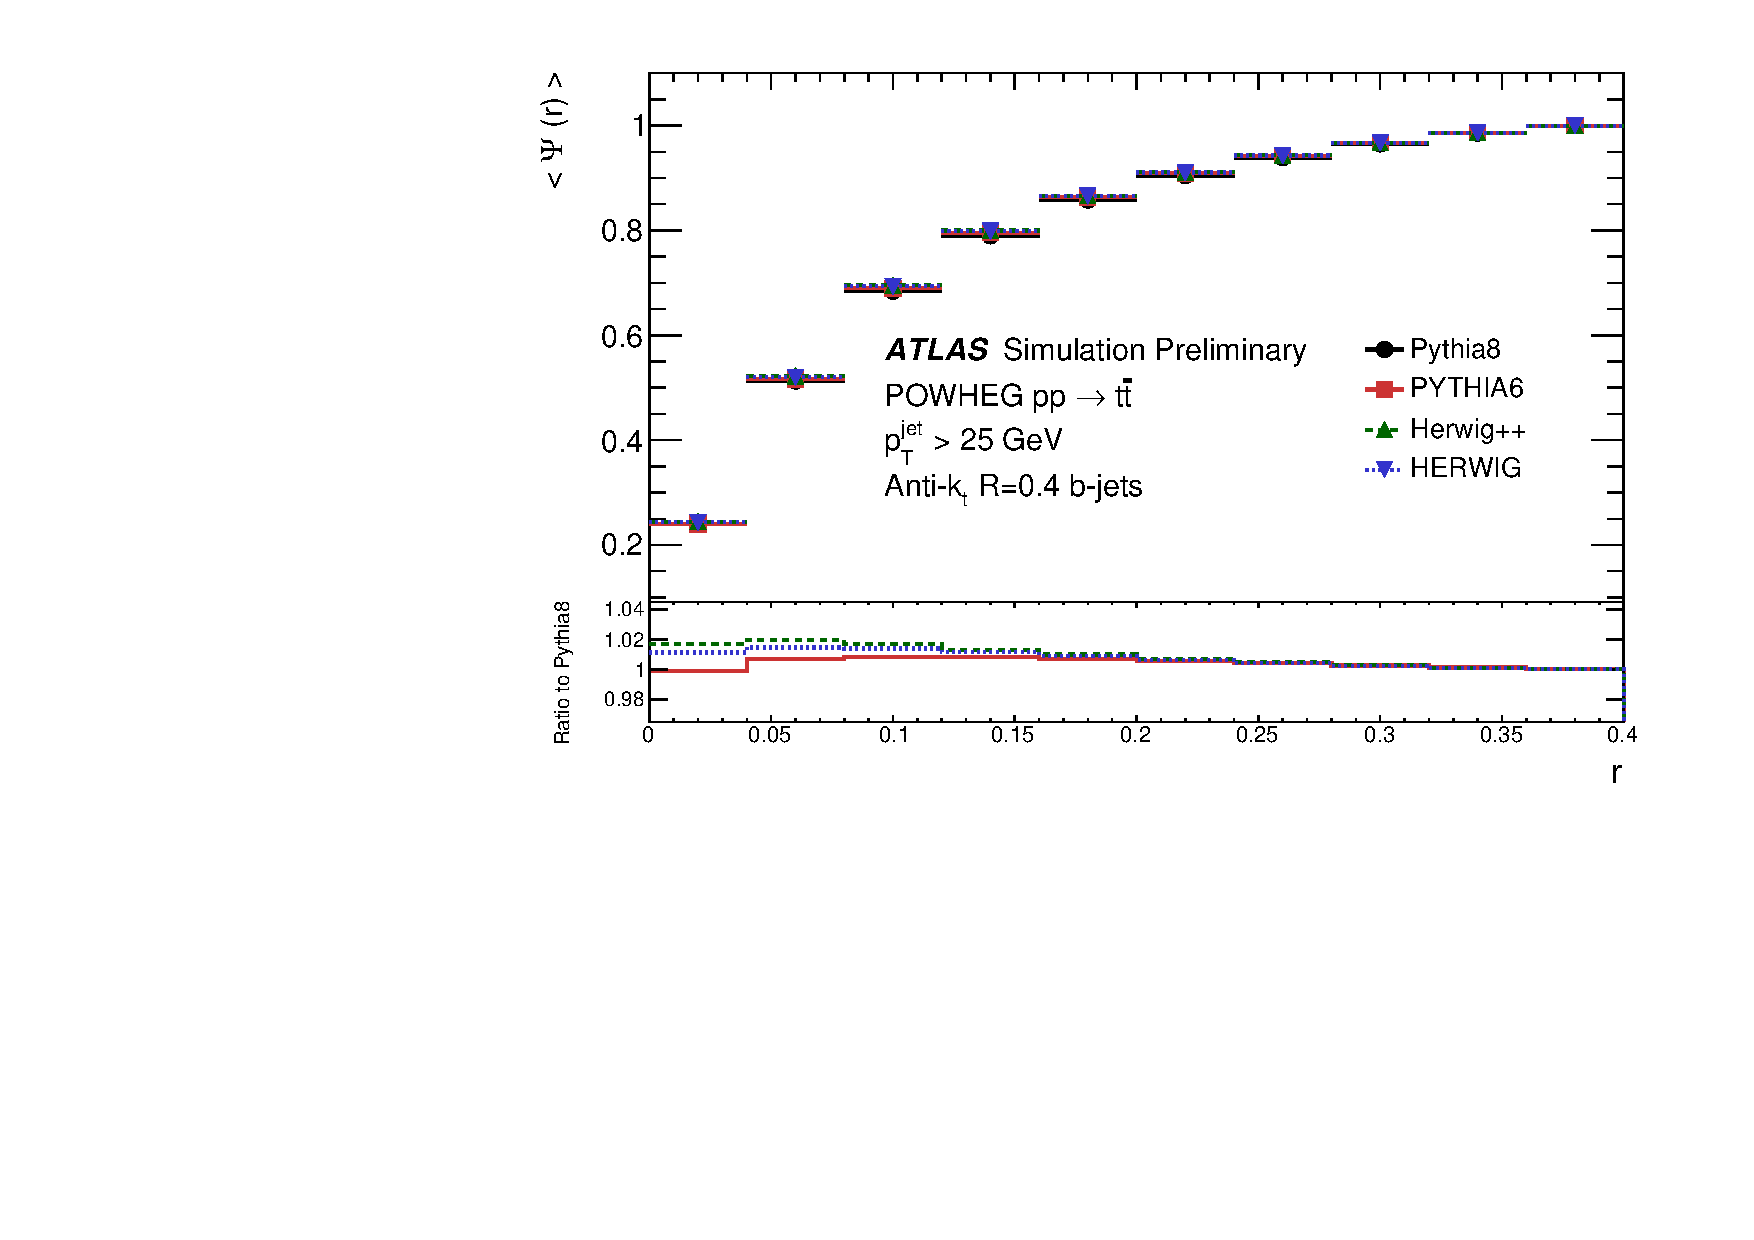
\includegraphics[width=\textwidth]{evtgen/figures/Frag/Top/SingleB/PsiVariableR.pdf}
\end{subfigure}
\begin{subfigure}[]{0.45\textwidth}
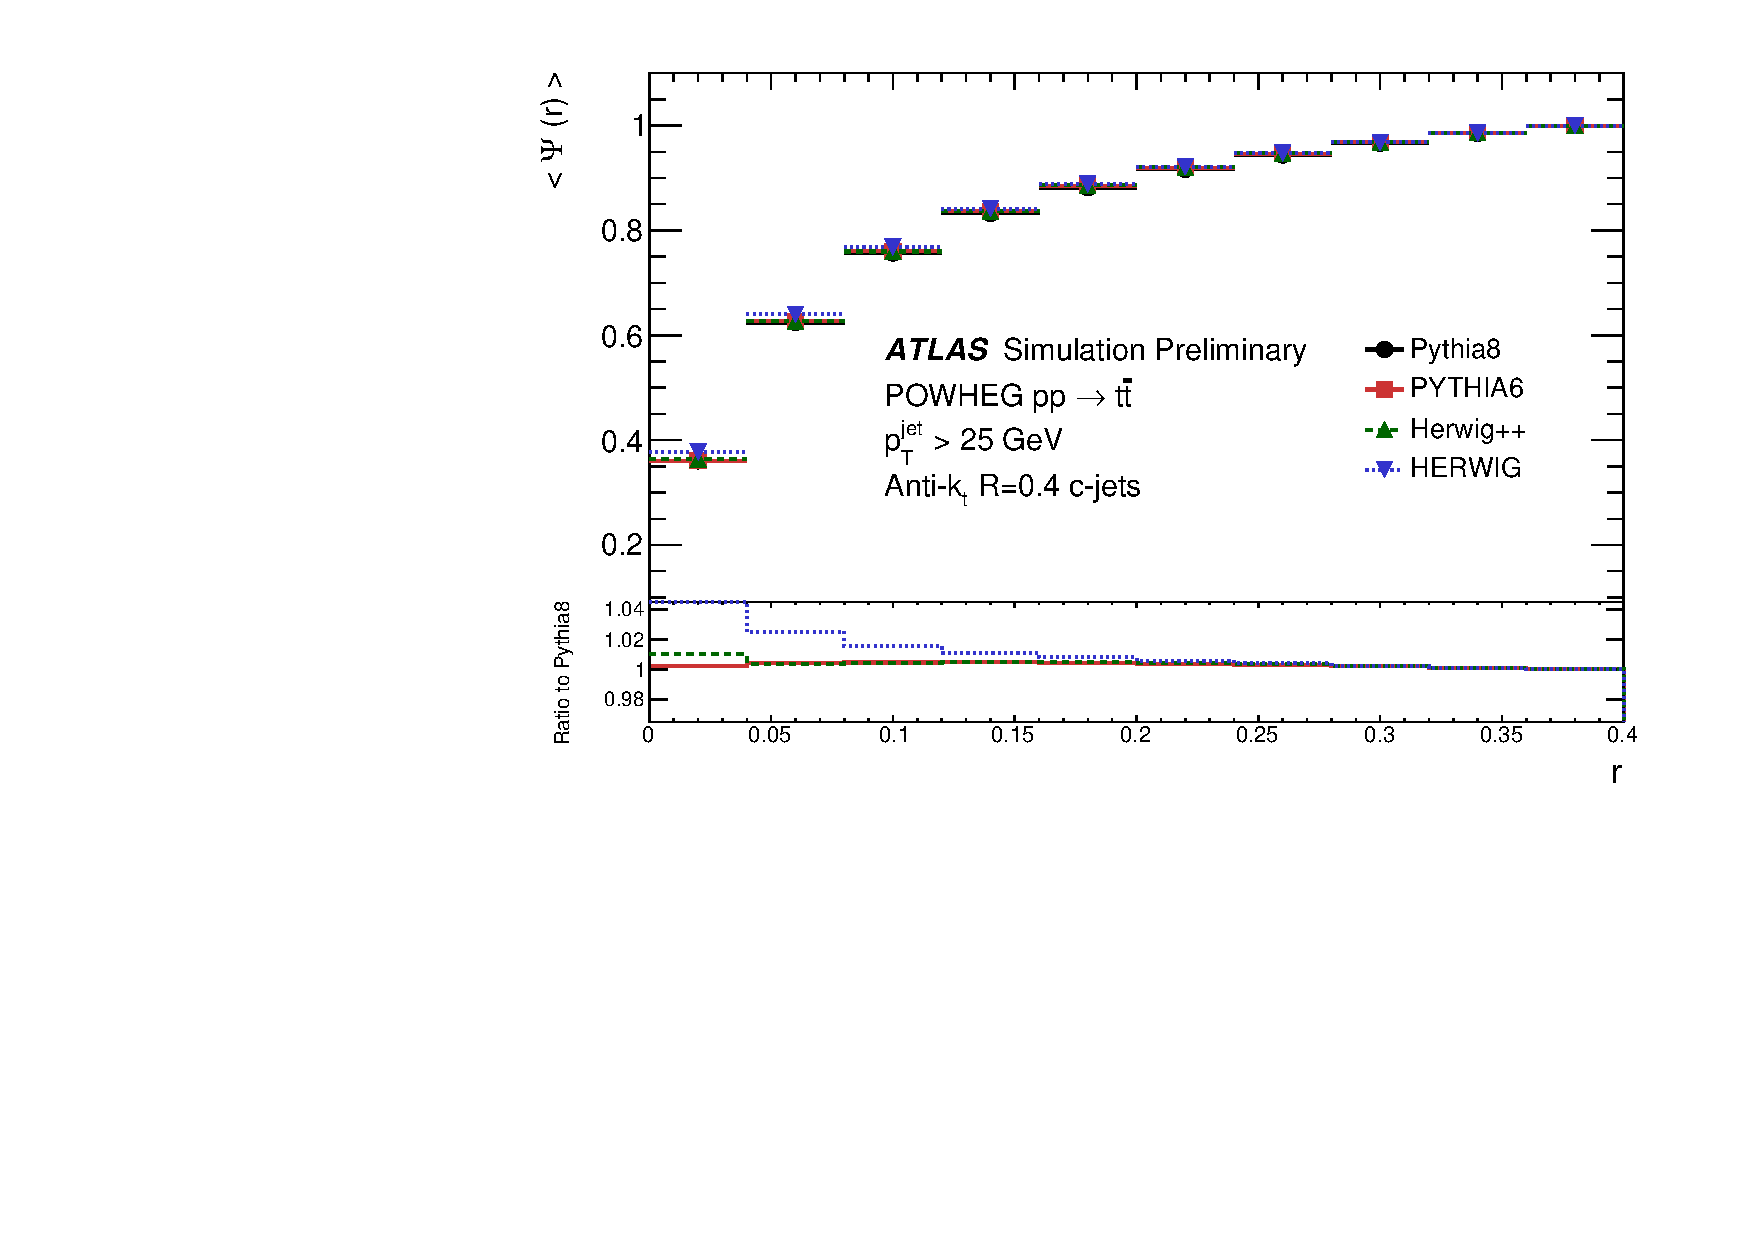
\includegraphics[width=\textwidth]{evtgen/figures/Frag/Top/SingleC/PsiVariableR.pdf}
\end{subfigure}
\caption{The integral jet shape 
$\Psi \left( r, R=0.4 \right ) \equiv  \Sigma p_T \left(0, r \right) \ \sum p_T \left(0, R \right) $ 
distribution for 
(a)~$b$-jets and (b)~$c$-jets in \PowHeg\
\ttbar\ samples where  \PythiaE, \Pythia, \Herwigpp\ and \Herwig\ have been used 
for the parton shower, hadronization and underlying event modeling. The legend includes the value and error of the mean of each distribution.}
\label{fig:tpsi}
\end{figure}



\begin{figure}
\centering
\begin{subfigure}[]{0.45\textwidth}
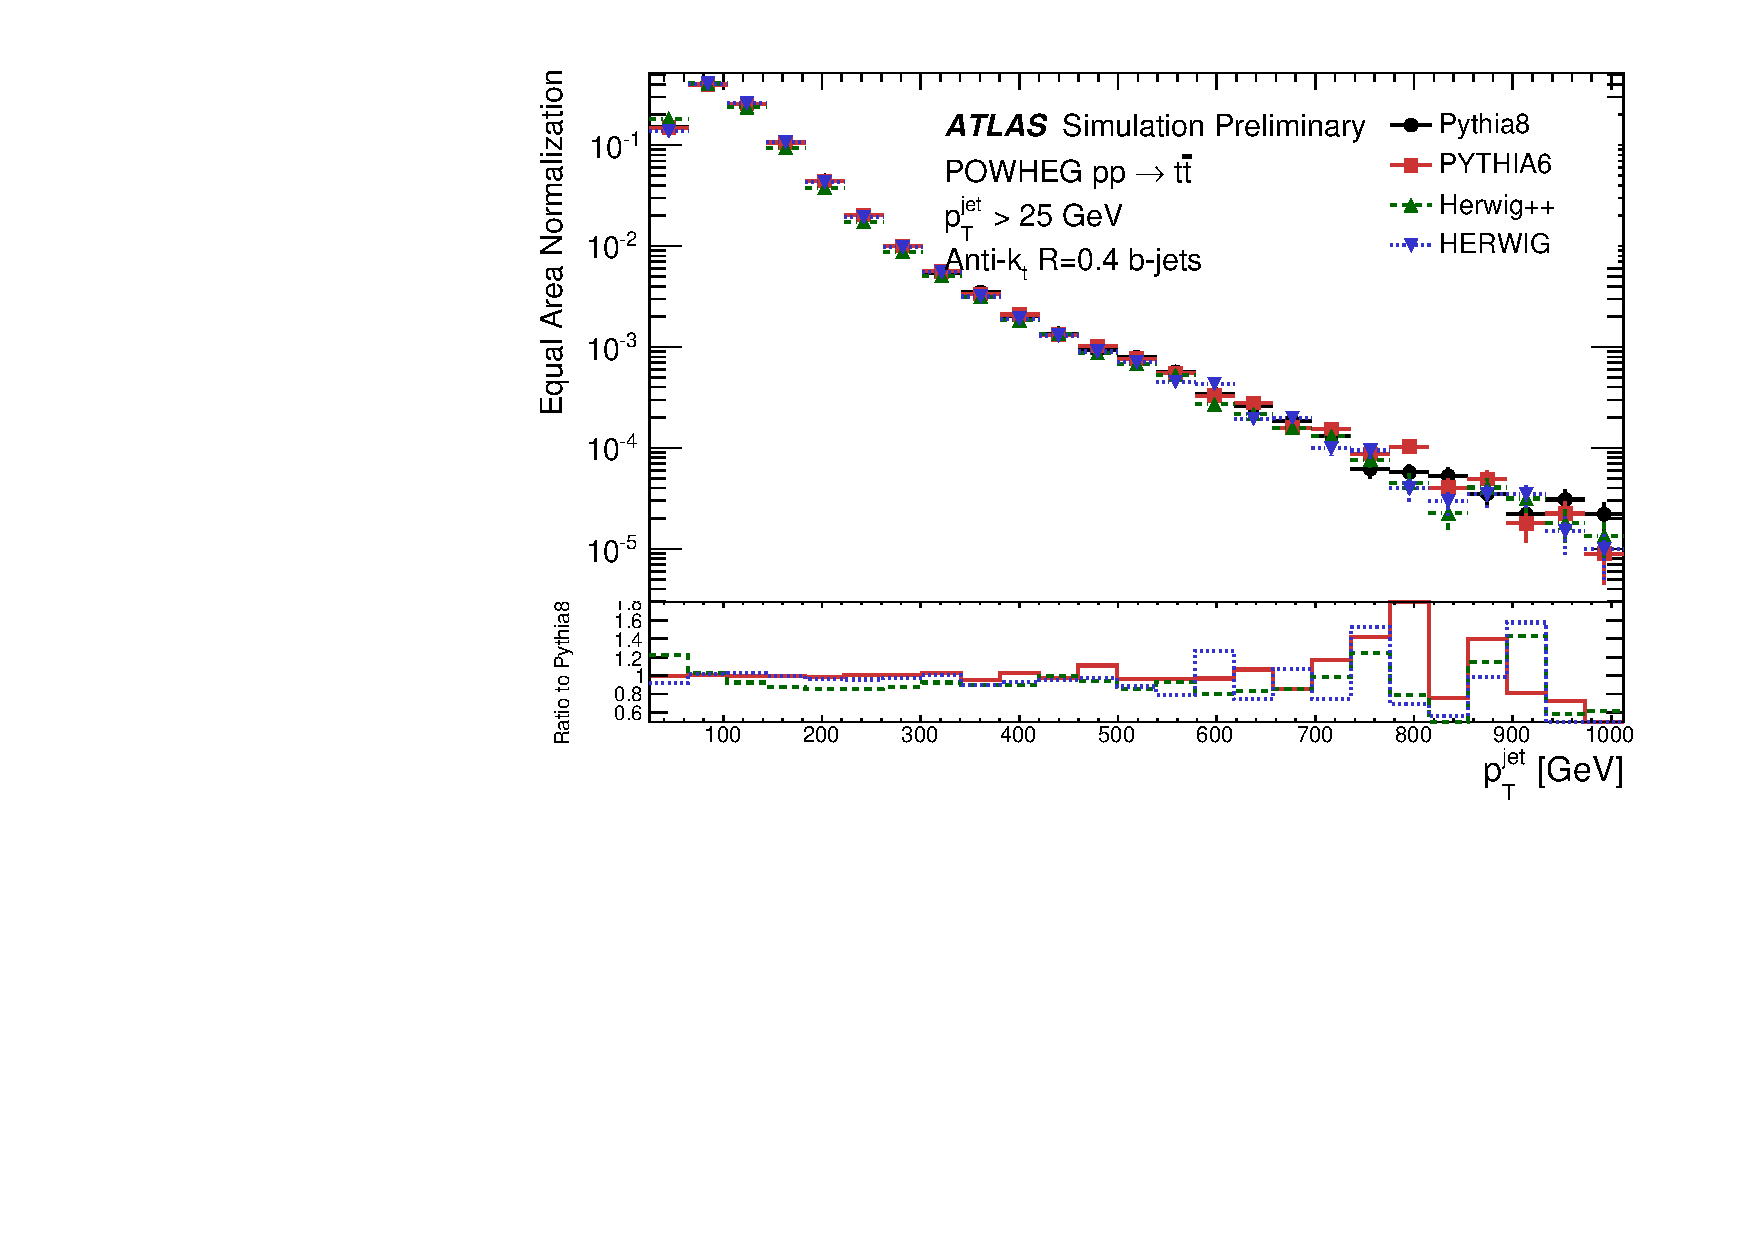
\includegraphics[width=\textwidth]{evtgen/figures/Frag/Top/SingleB/h_JetpT.pdf}
\end{subfigure}
\begin{subfigure}[]{0.45\textwidth}
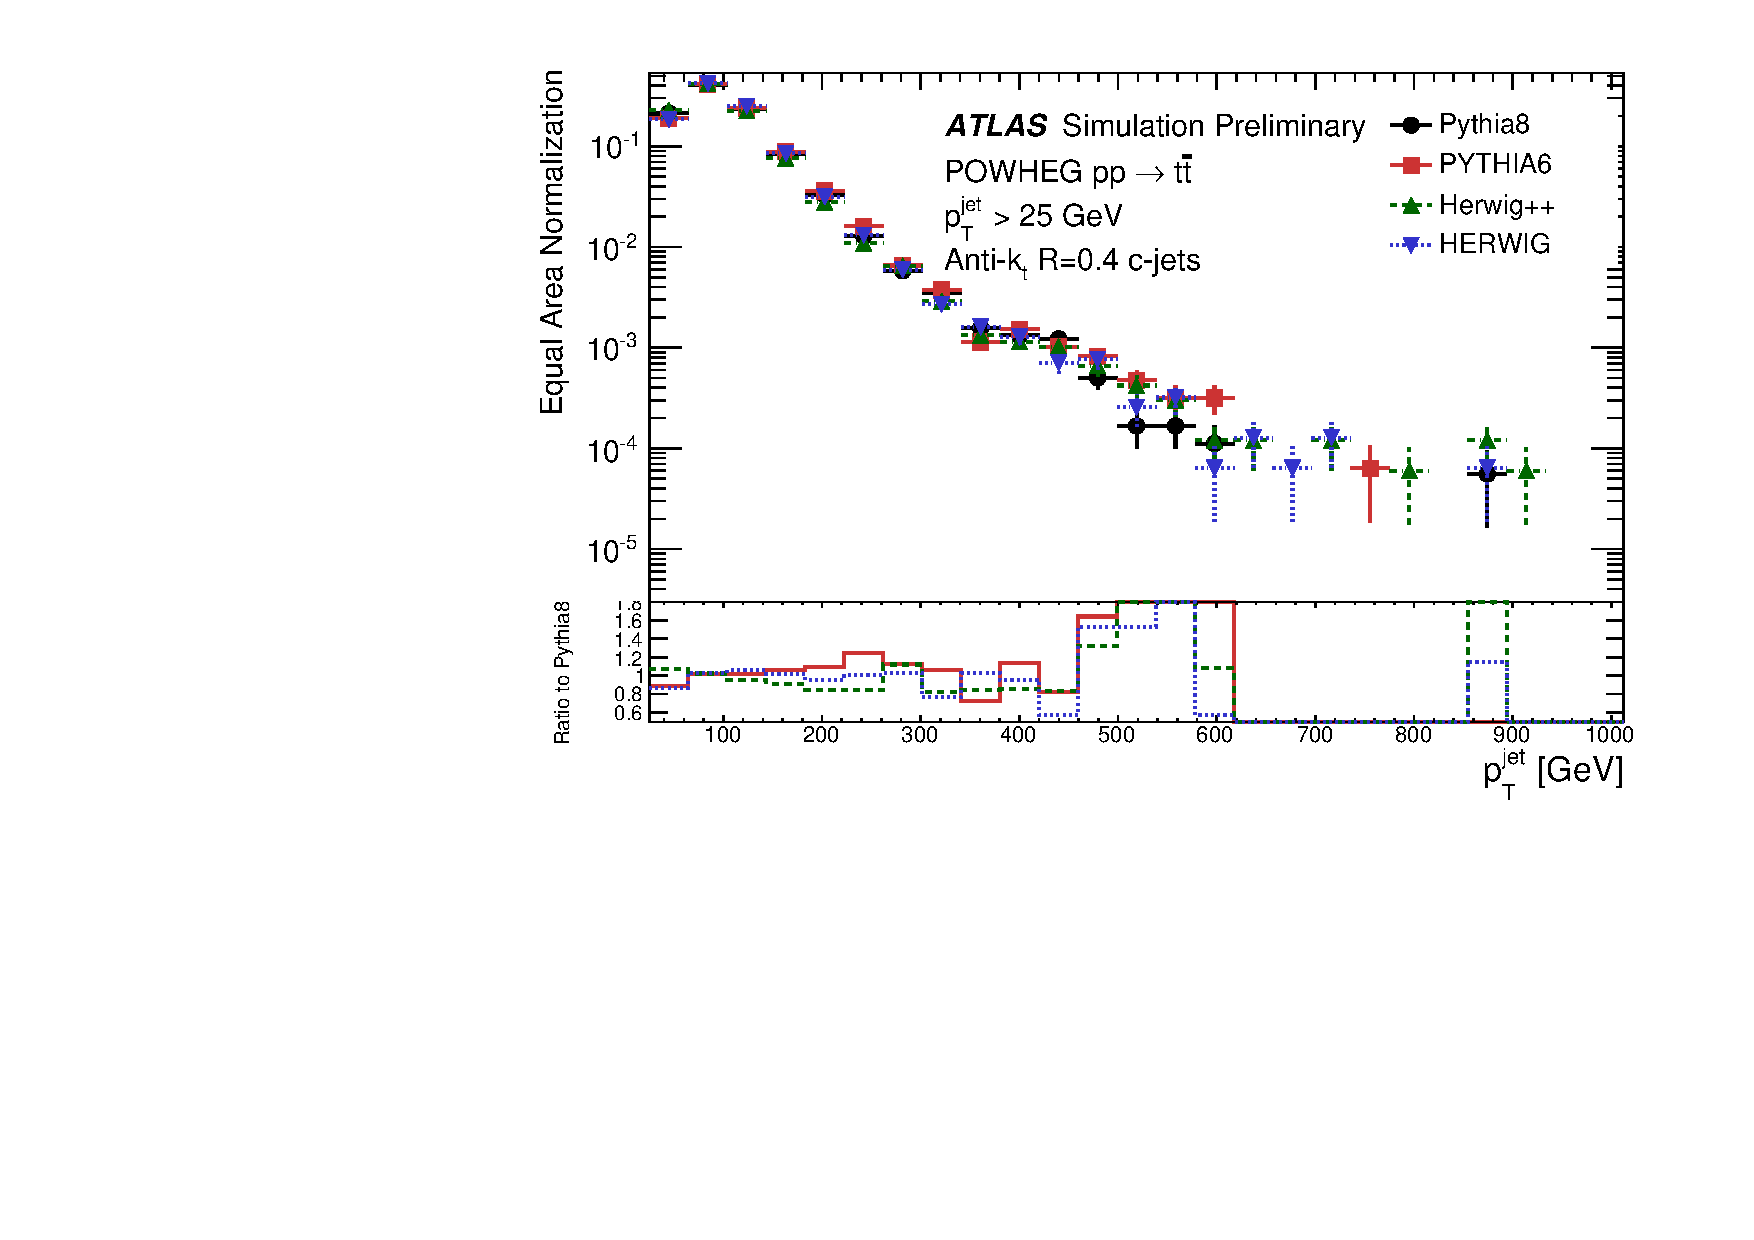
\includegraphics[width=\textwidth]{evtgen/figures/Frag/Top/SingleC/h_JetpT.pdf}
\end{subfigure}
\caption{The \ptJet\ distribution for 
(a)~$b$-jets and (b)~$c$-jets in \PowHeg\
\ttbar\ samples where  \PythiaE, \Pythia, \Herwigpp\ and \Herwig\ have been used 
for the parton shower, hadronization and underlying event modeling.}
\label{fig:tjpt}
\end{figure}

\begin{figure}
\centering
\begin{subfigure}[]{0.45\textwidth}
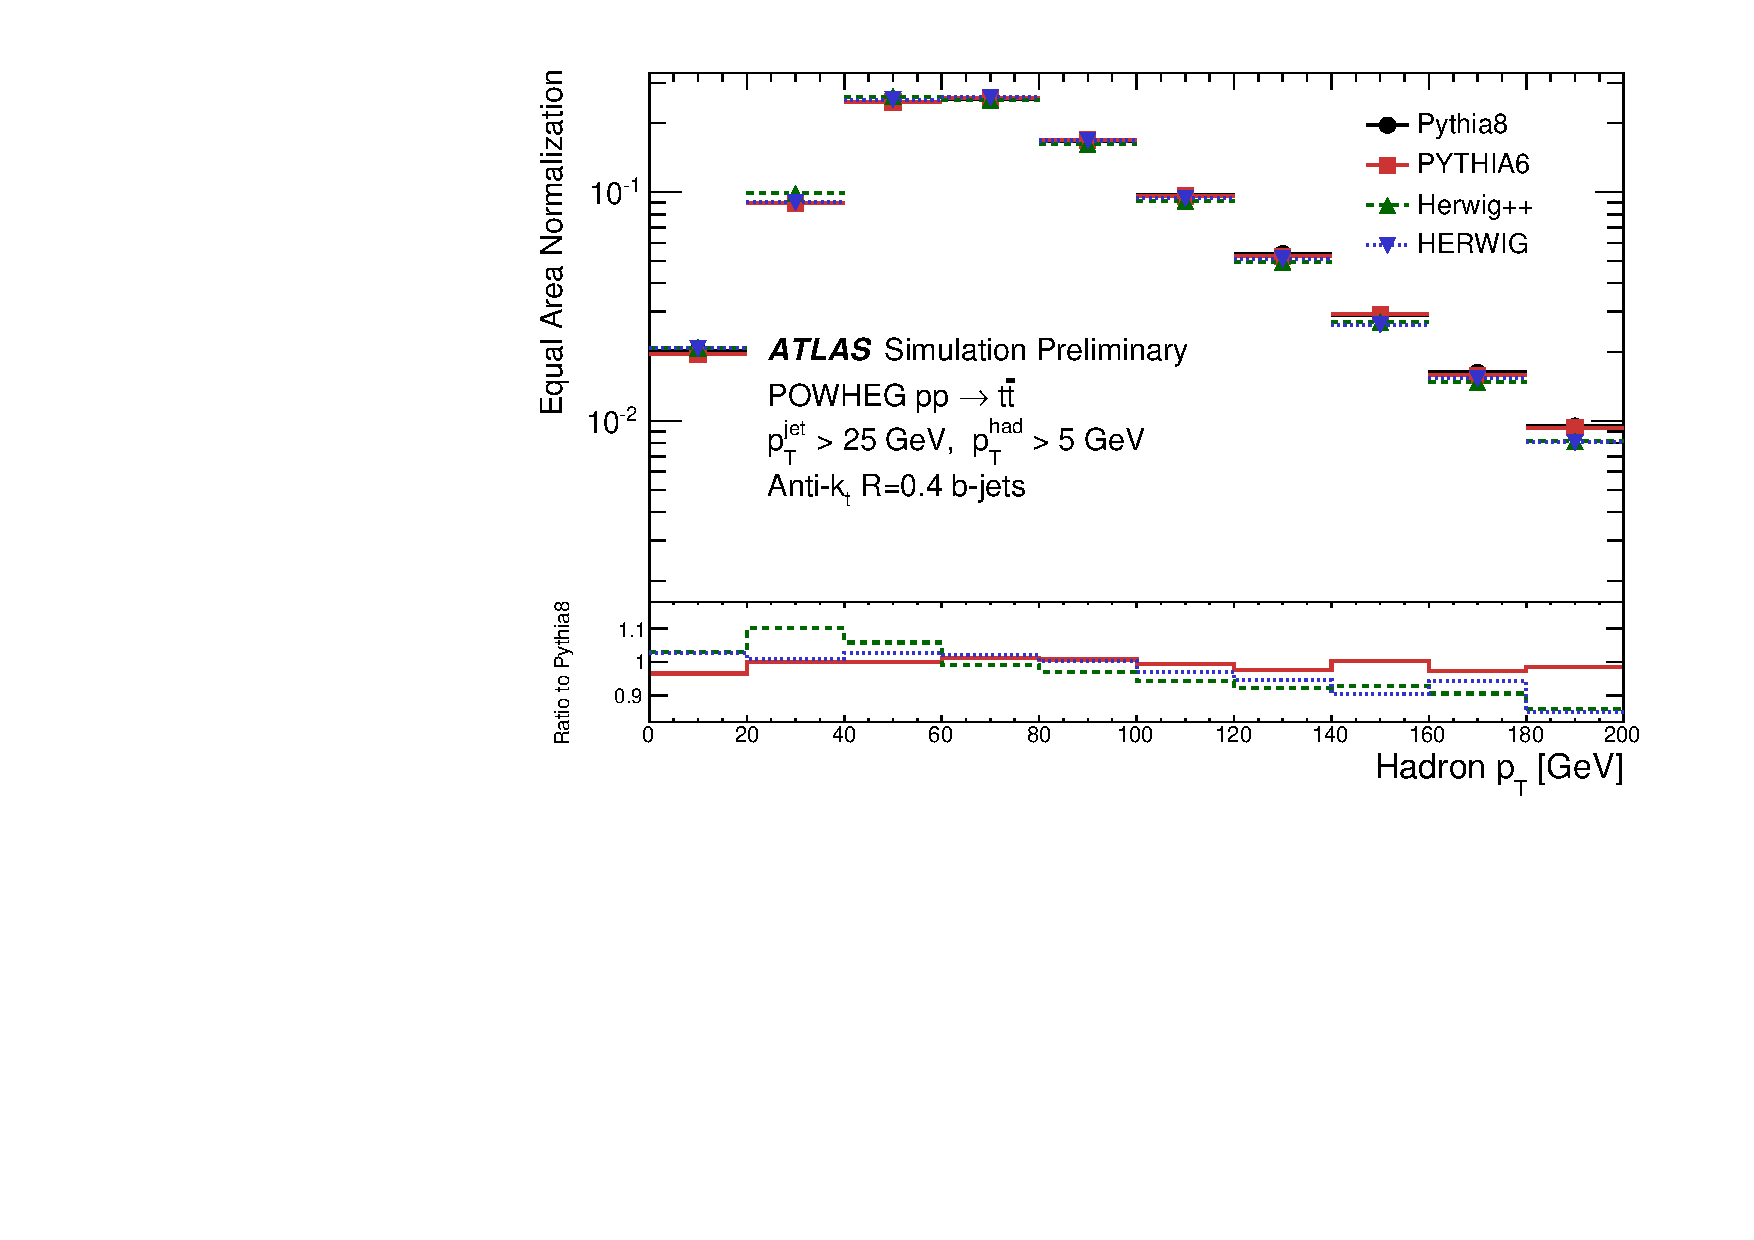
\includegraphics[width=\textwidth]{evtgen/figures/Frag/Top/SingleB/h_HardHadpT.pdf}
\end{subfigure}
\begin{subfigure}[]{0.45\textwidth}
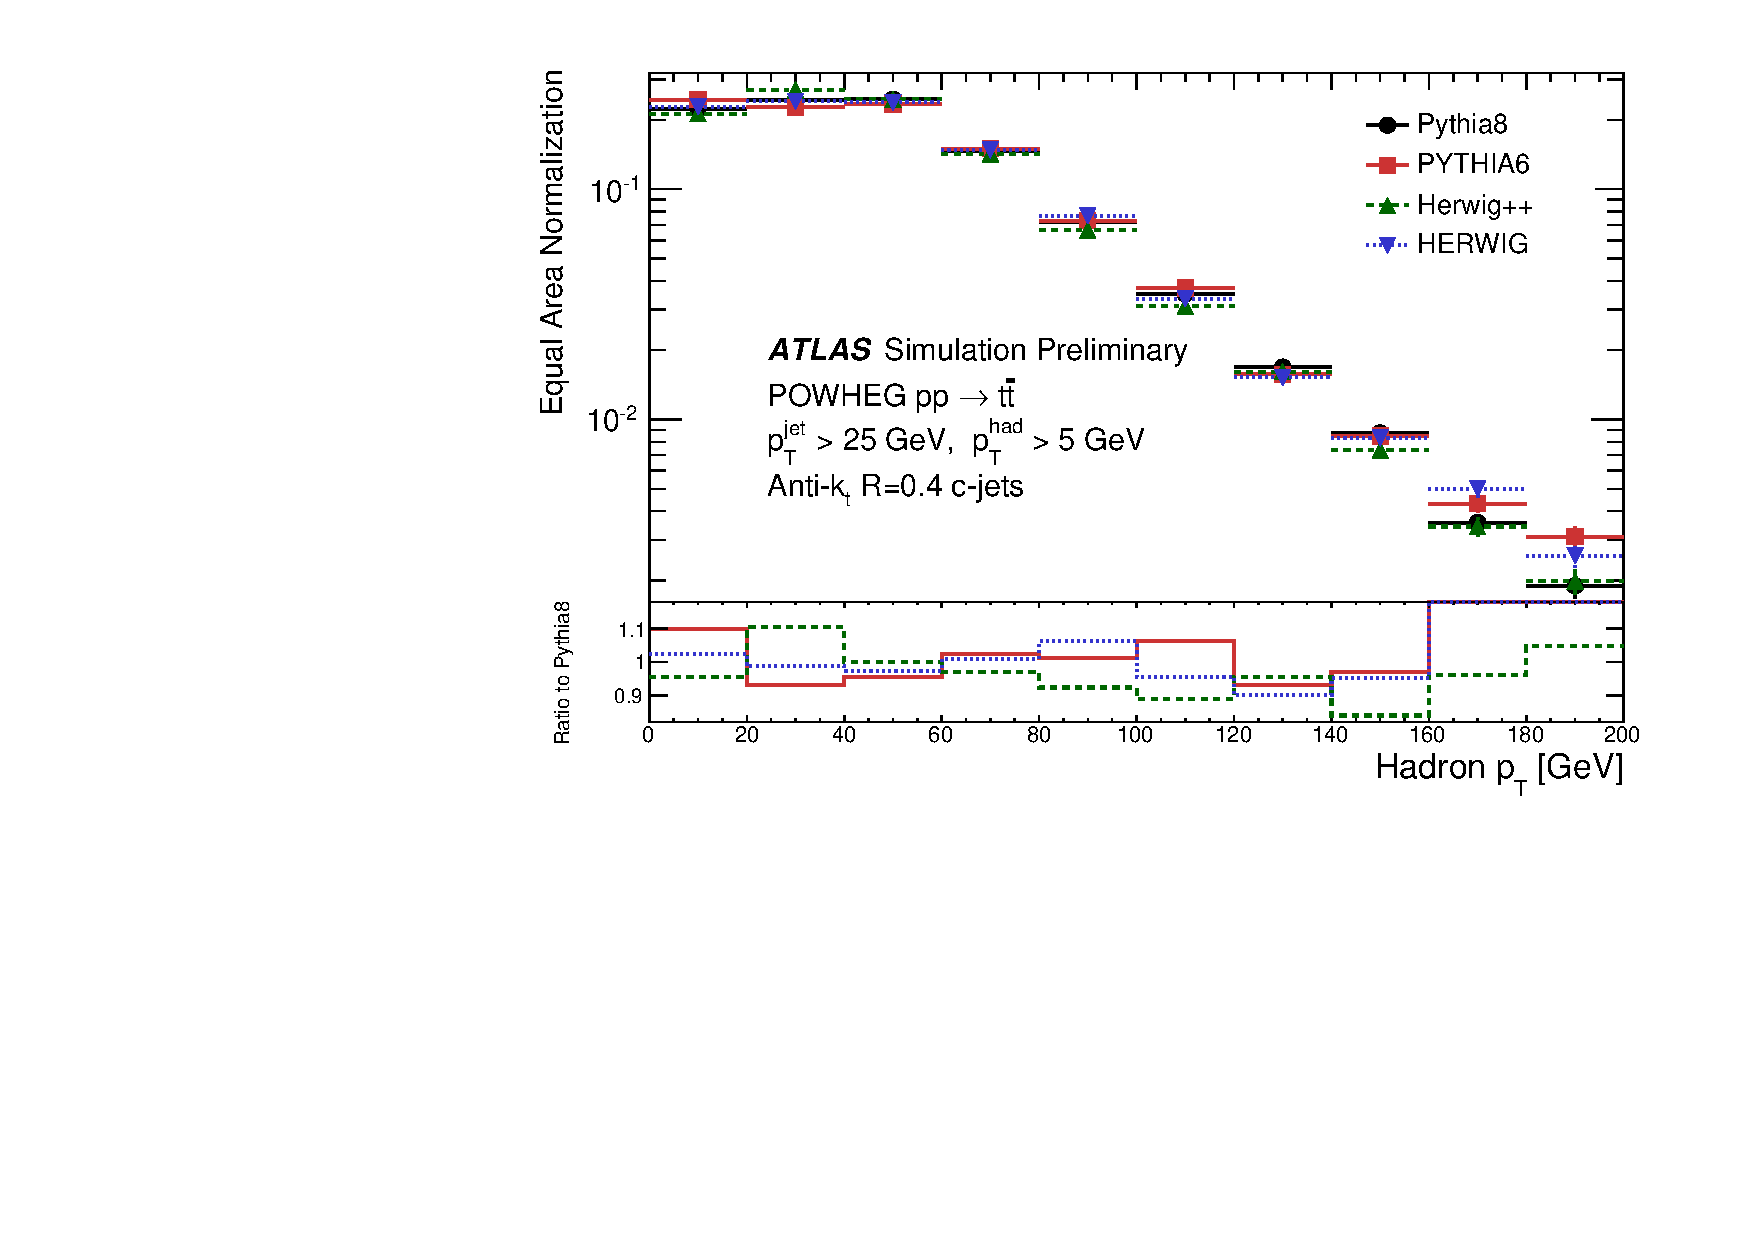
\includegraphics[width=\textwidth]{evtgen/figures/Frag/Top/SingleC/h_HardHadpT.pdf}
\end{subfigure}
\caption{The \ptHad\ distribution for 
(a)~$b$-jets and (b)~$c$-jets in \PowHeg\
\ttbar\ samples where  \PythiaE, \Pythia, \Herwigpp\ and \Herwig\ have been used 
for the parton shower, hadronization and underlying event modeling.}
\label{fig:thadpt}
\end{figure}


\begin{figure}
\centering
 \begin{subfigure}[]{0.45\textwidth}
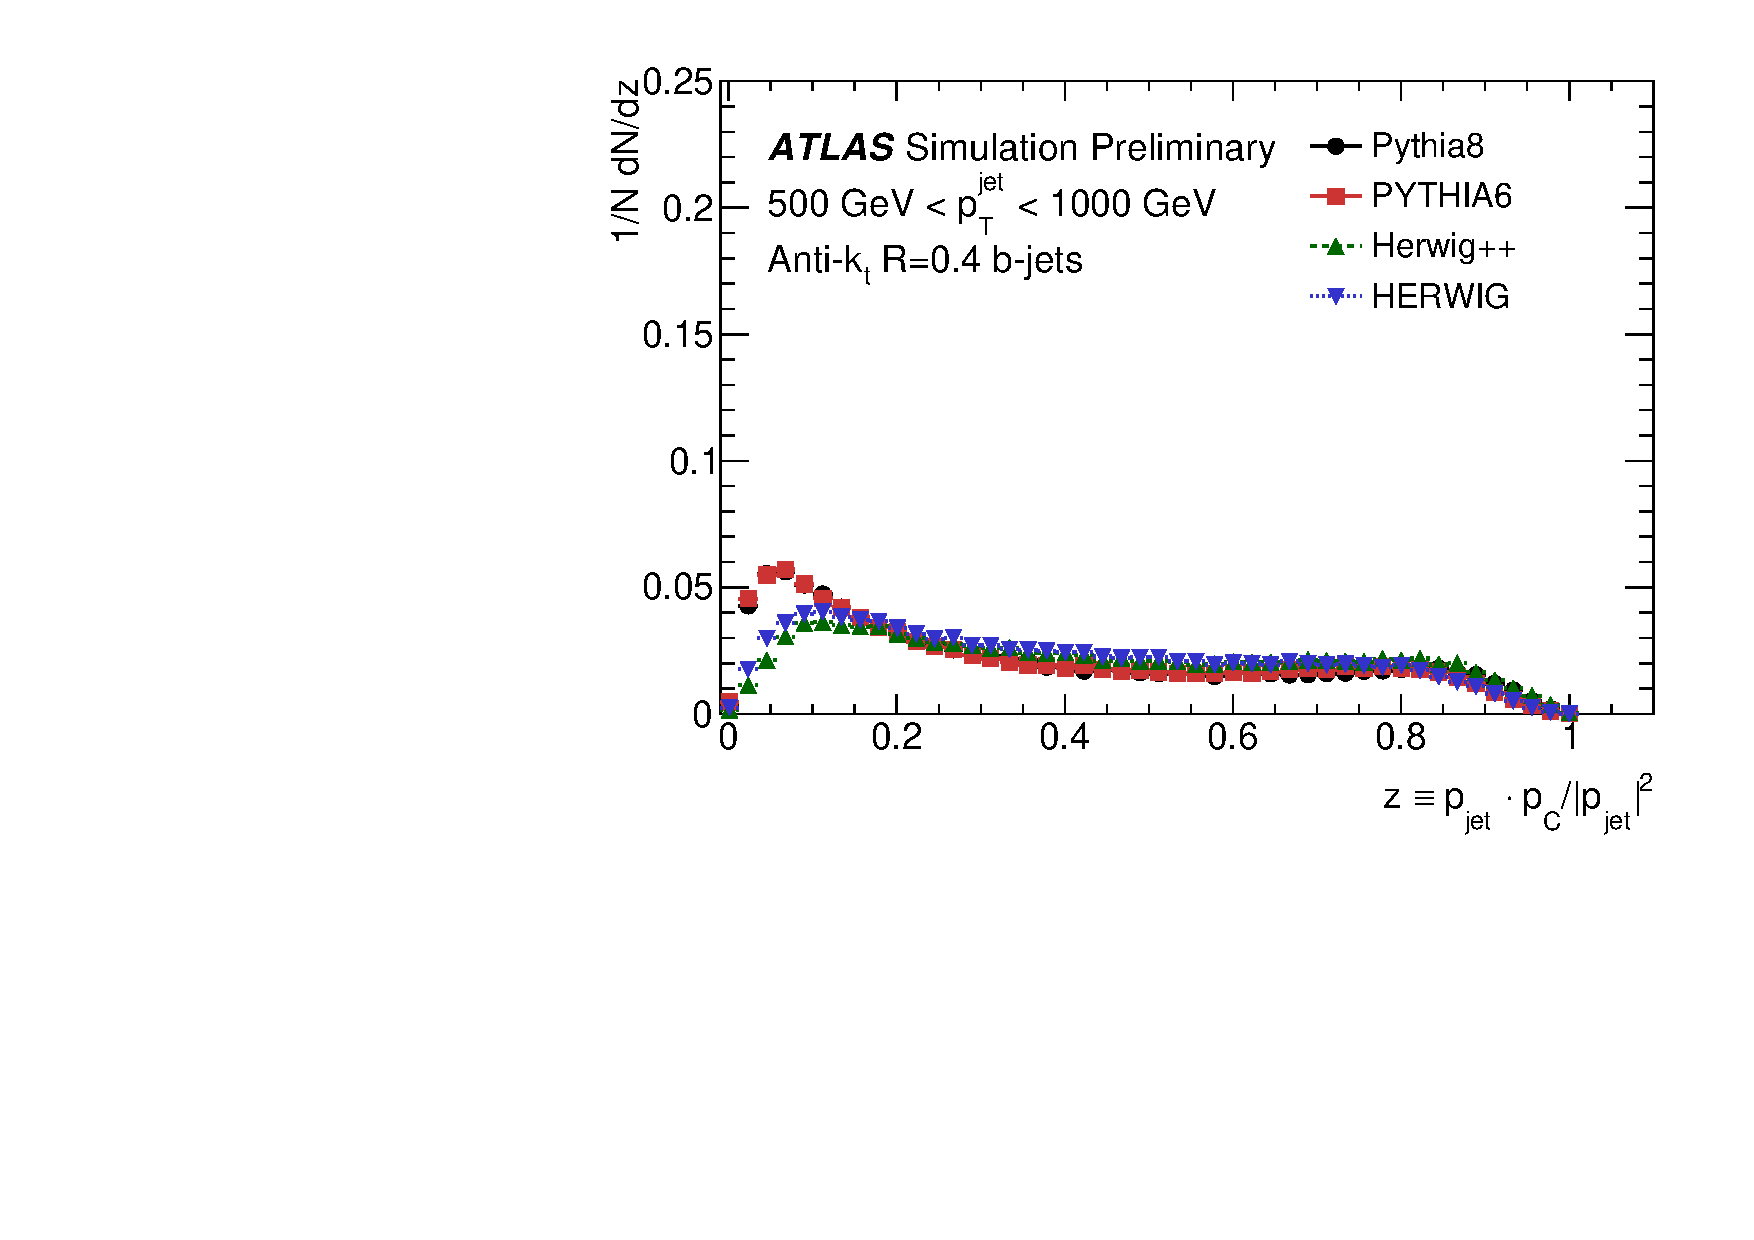
\includegraphics[width=\textwidth]{evtgen/figures/Frag/Jz4/WithIsolation/h_BFrag.pdf}
\end{subfigure}
 \begin{subfigure}[]{0.45\textwidth}
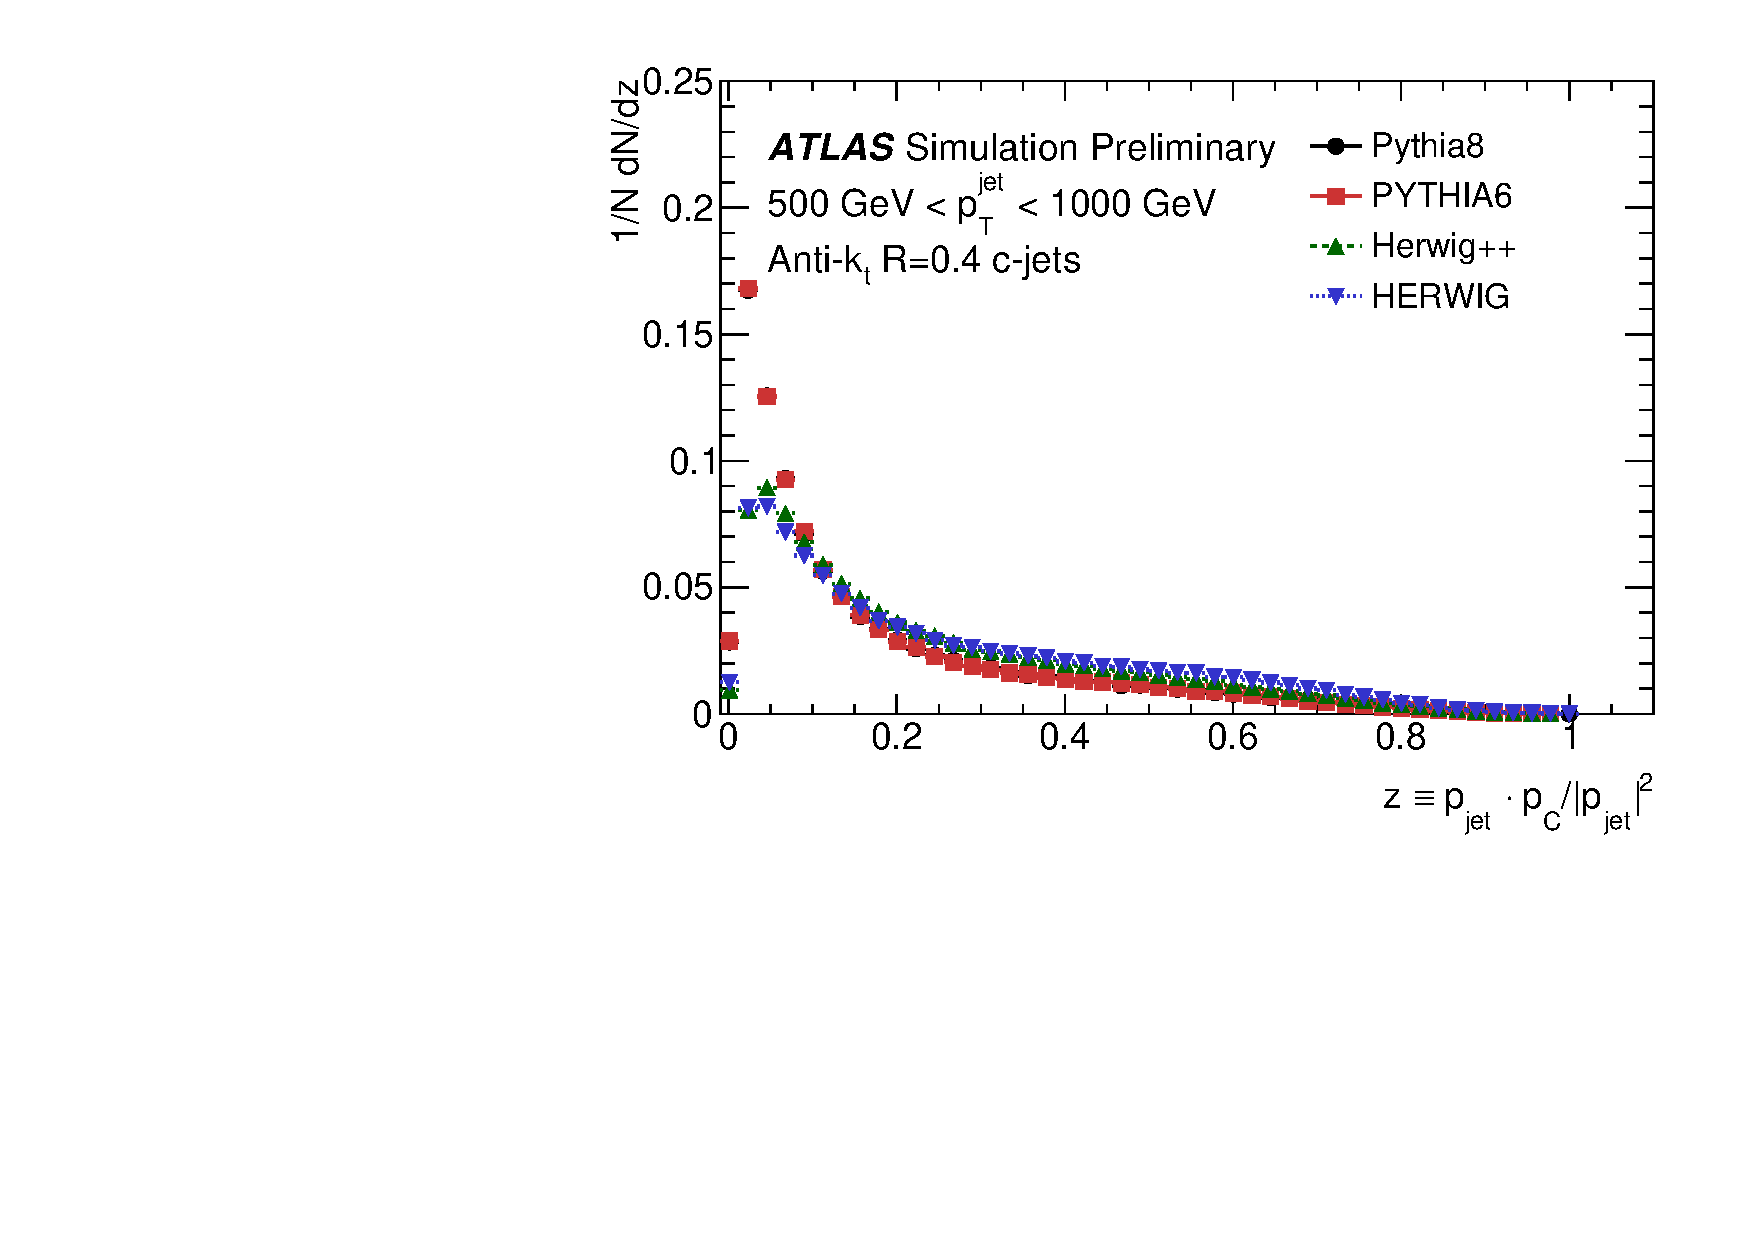
\includegraphics[width=\textwidth]{evtgen/figures/Frag/Jz4/WithIsolation/h_CFrag.pdf}
\end{subfigure}
  \begin{subfigure}[]{0.45\textwidth}
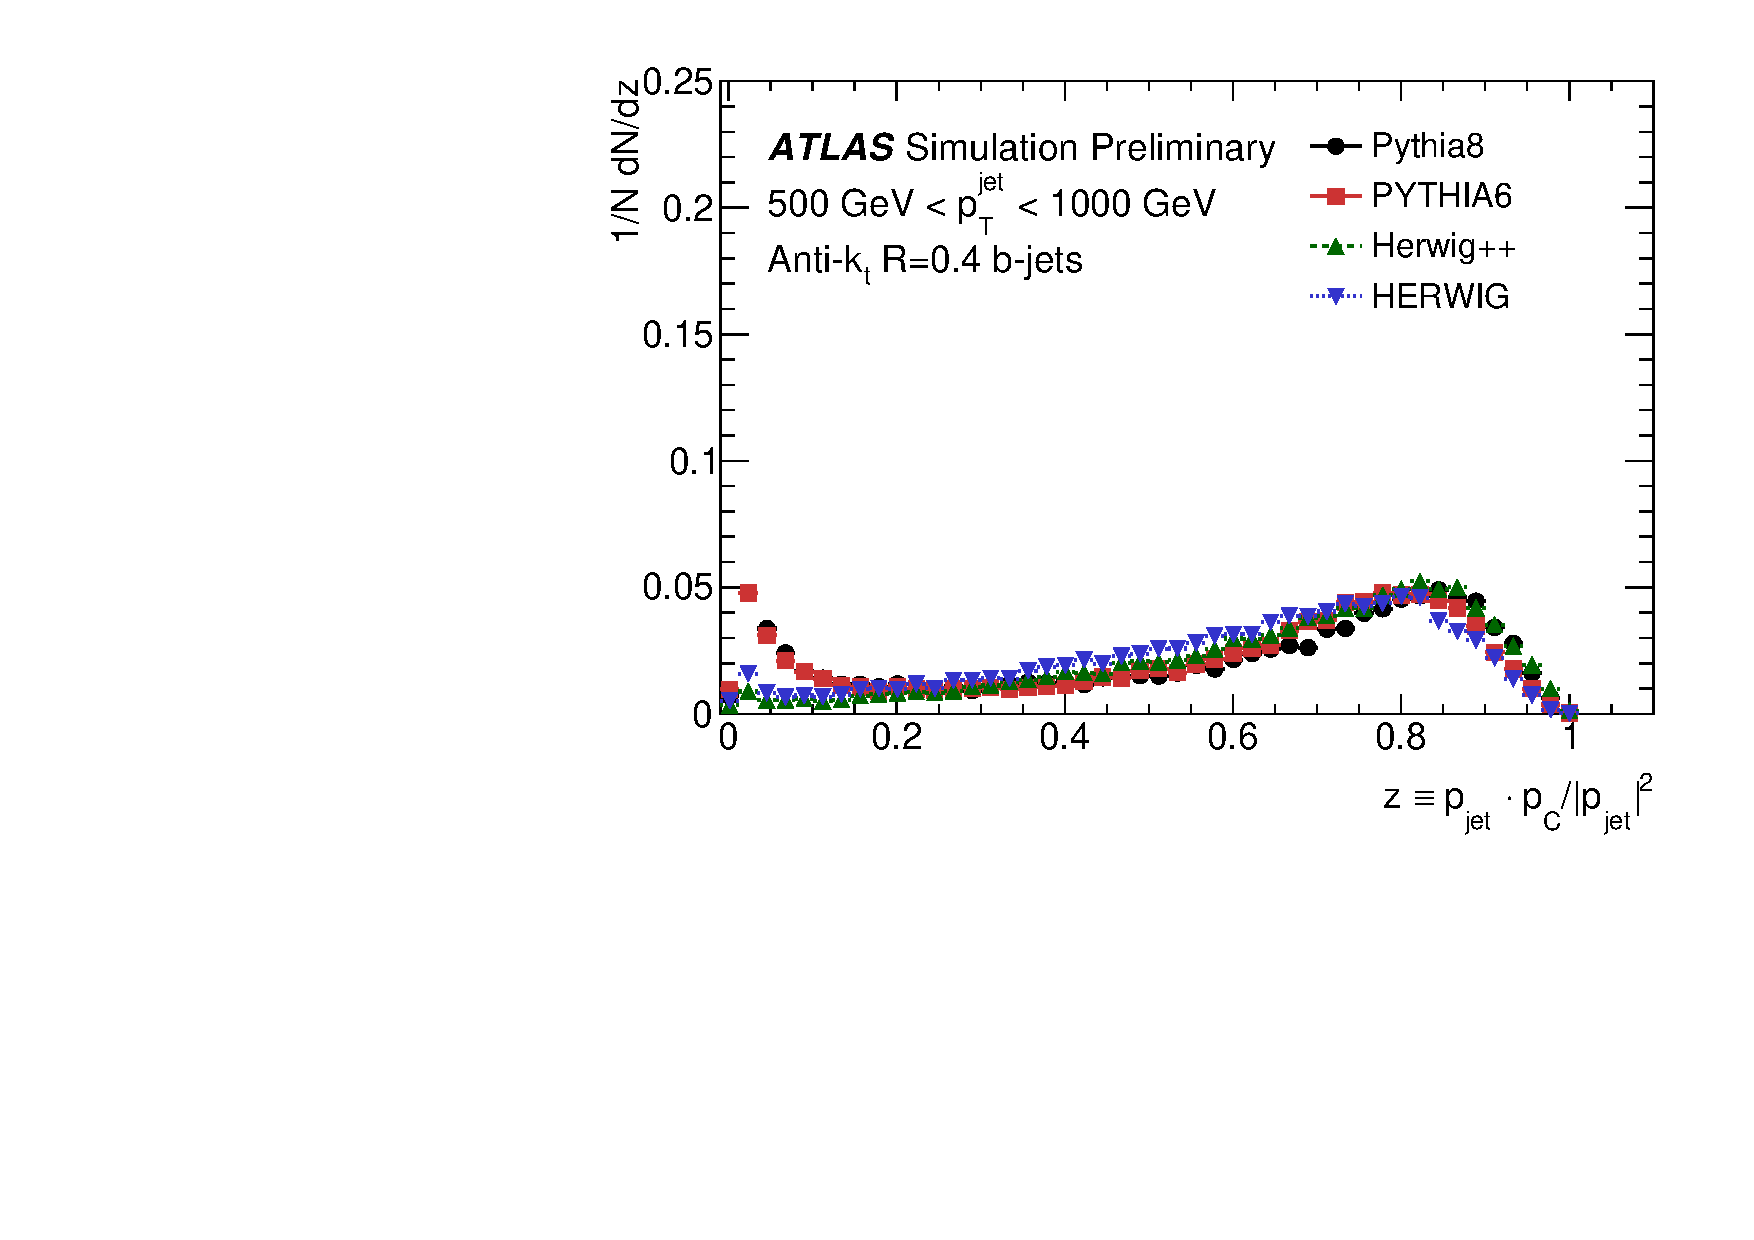
\includegraphics[width=\textwidth]{evtgen/figures/Frag/Jz4/WithIsolation/h_BFrag_SingleHad.pdf}
\end{subfigure}
 \begin{subfigure}[]{0.45\textwidth}
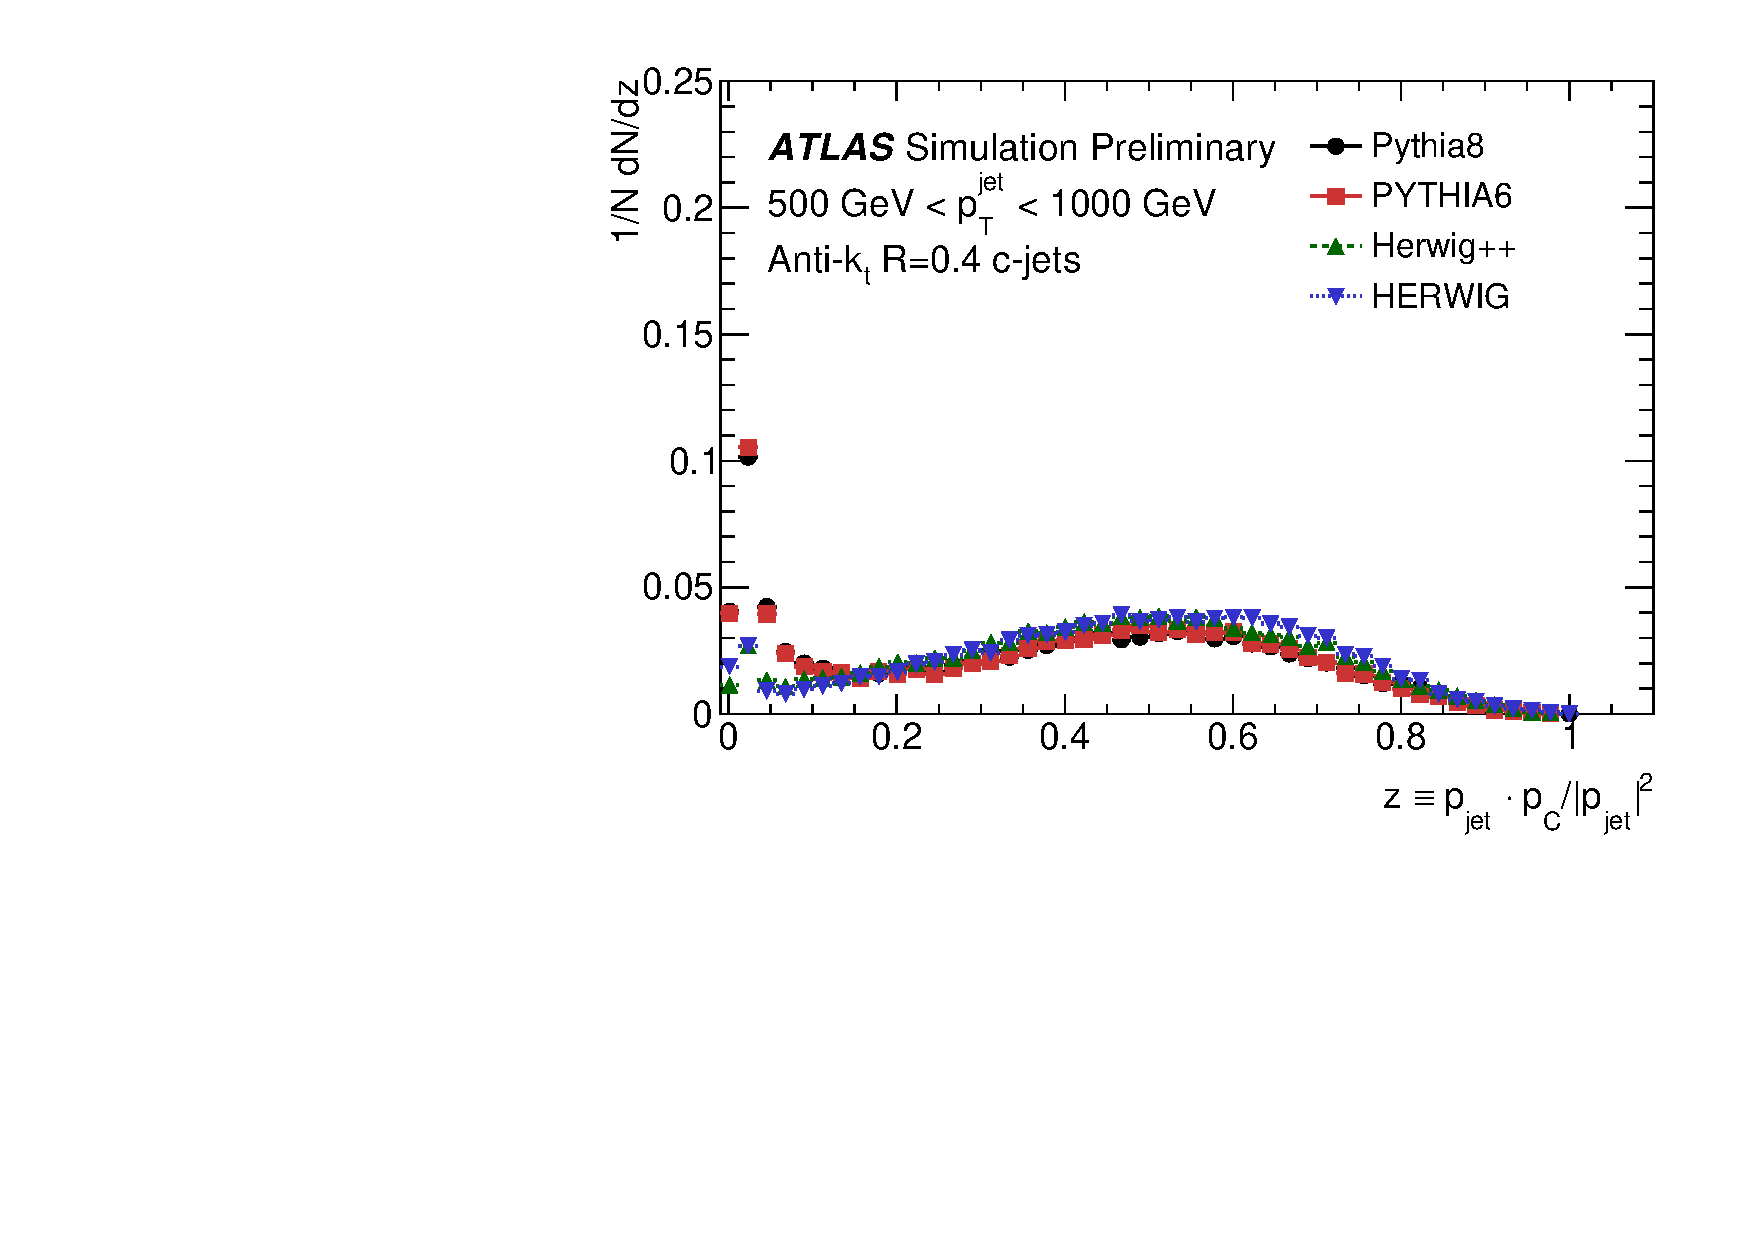
\includegraphics[width=\textwidth]{evtgen/figures/Frag/Jz4/WithIsolation/h_CFrag_SingleHad.pdf}
\end{subfigure}

\caption{The fragmentation function for (a)~$b$-jets and (b)~$c$-jets in the 
high \pT\ jet sample and for the subset
of (c)~$b$-jets and (d)~$c$-jets containing exactly one heavy flavor hadron.
}
\label{fig:jz4frag}
\end{figure}
\begin{table}
\subfloat[][All jets]{
\centering
\begin{tabular}{|r|r|r|}
\hline
Generator & $p_{jet} \cdot p_{B}/p_{jet}^2$  & $p_{jet} \cdot p_{C}/p_{jet}^2$ \\
\hline
 \PythiaE & $0.3683 \pm 0.0012$   & $0.1853 \pm 0.0004$    \\
 \Pythia & $0.3633 \pm 0.0010$  & $0.1841 \pm 0.0004$ \\
 \Herwigpp & $0.4356 \pm 0.0011$   & $0.2442 \pm 0.0005$    \\
 \Herwig  & $0.3984 \pm 0.0011$   & $0.2614 \pm 0.0006$   \\
\hline
\end{tabular}
}
\hfill
\subfloat[][Single heavy flavor hadron jets]{
\centering
\begin{tabular}{|r|r|r|}
\hline
Generator & $p_{jet} \cdot p_{B}/p_{jet}^2$  & $p_{jet} \cdot p_{C}/p_{jet}^2$ \\
\hline
 \PythiaE & $0.5747 \pm 0.0022$  & $0.3790 \pm 0.0018$   \\
 \Pythia & $0.5696 \pm 0.0019$  & $0.3787 \pm 0.0016$ \\
 \Herwigpp & $0.6473 \pm 0.0017$  &$0.4549 \pm 0.0015$   \\
 \Herwig  & $0.5953 \pm 0.0017$  & $0.4674 \pm 0.0015$   \\
\hline
\end{tabular}
}
\caption{The mean fragmentation function for (a)~$b$-jets and $c$-jets in the 
high \pT~jet sample and for the subset
of (b)~$b$-jets and ~$c$-jets 
satisfying the additional requirement that there be no other weakly decaying
heavy flavor hadron with $\pt>5.0$~\GeV\ within a cone $\Delta R=1$ of the jet.}
\label{t:jz4frag}
\end{table}
The differential jet shape $\rho (r)$ in an annulus of inner radius $r-\Delta r /2$ and outer radius $r+\Delta r /2$ from the axis~\footnote{The jet axis is defined to be the direction of the momentum vector of the jet from the \antiktfour\ algorithm.} of a given jet is defined as

$$
\rho(r) = \frac{1}{\Delta r} \frac{p_T \left(r-\Delta r /2, r+\Delta r /2 \right)}{p_T \left(0, R \right)}
$$ 
\noindent
Here $\Delta r = 0.04$ is the width of the annulus, $r$, such that $\Delta r /2 \leq r \leq R - \Delta r /2$ is the distance to the jet axis in the $\eta-\phi$ plane and $p_T(r_1, r_2)$ is the scalar sum of the $p_T$ of the jet constituents with radii between $r_1$ and $r_2$. Figure~\ref{fig:trho} shows the distribution of the variable $\rho(r)$. 
ATLAS results for \ttbar\ production at 7~\TeV\ indicate that \PowHeg\ with \Pythia\ for the parton shower give
good agreement with the data for this variable~\cite{Aad:2013fba}. No experimental results are currently available at 8~\TeV.

The integrated jet shape in a cone of radius $r<R$ around the jet axis is defined as the cumulative distribution for $\rho(r)$, i.e.

$$
\Psi(r) \equiv \frac{p_T \left(0, r \right)}{p_T \left(0, R \right)},\; 0 \leq r \leq R 
$$
\noindent
which satisfies $\Psi(r = R) = 1$.
Figure~\ref{fig:tpsi} shows the distribution of $\Psi(r)$. For each of these jet shapes, differences between the 
generators are small. The fact that \Herwigpp\ (\Herwig) $b$-quark ($c$-quark) fragmentation is harder than for the other generators is not clearly explained by differences in the the $W$, $\rho(r)$ or $\Psi(r)$ distributions.

Figure~\ref{fig:tjpt} shows the jet \pT\ distribution for $b$- and  $c$-jets in the \ttbar\ samples.
For $b$-jets, the generators are in reasonable agreement, except for \Herwigpp, which exhibits a slightly softer
spectrum.  All generators agree well for $c$-jets.  Figure~\ref{fig:thadpt} shows the \pT\ distributions
of the bottom and charm hadrons contained in these jets.  \Herwigpp\ produces a slightly
softer \pT\ spectrum for the bottom hadrons, while \Herwig\ has a softer spectrum for charm hadrons.  
%%These distributions suggest that the differences in $f(z)$ come from largely the modeling of the fragmentation itself.

For high \pT\ jets, the $f(z)$ distribution has two components. The fragmentation of heavy flavor created in the hard scatter produces a distribution at higher $z$. The production of heavy flavor in additional processes gives a component at lower $z$. Examples of such processes include gluon splitting, multiple parton interactions and heavy flavor production within the hadronization process.  These components have been studied for jets with
\ptJet\ between 500~\GeV\ and 1~\TeV. Figures~\ref{fig:jz4frag}~(a) and~\ref{fig:jz4frag}~(b) show the distribution of $f(z)$ for the four generators for $b$- and  $c$-jets respectively.  The dominant feature in these distributions is a large peak at low $z$, although this peak is less pronounced for \Herwig\ and \Herwigpp\ than for \Pythia\ and \PythiaE. To enhance the high $z$ contribution from the hard scatter, the distributions are examined
in Figures~\ref{fig:jz4frag}~(c) and (d) for the subset of $b$- and  $c$-jets satisfying an additional requirement that there be no other weakly decaying heavy flavor hadron with $\ptHad>5.0$~\GeV\ within a cone $\Delta R=1$ of the jet.  While some evidence of the low $z$ peaking still remains, the distributions for $z>0.2$ in Figures~\ref{fig:jz4frag}~(c) and (d) are qualitatively similar to those of Figures~\ref{fig:tfrag}~(a) and (b) respectively.
\clearpage


%\section{Heavy Flavor Decays}
%\label{sec:decay}
%Heavy flavor decay properties are studied for different Monte Carlo
generators.
All weakly decaying bottom and charm hadrons (listed in Section~\ref{sec:prod}) were selected from inclusive \ttbar\ events and their decays were then analyzed. 

\PythiaE, \Pythia, \Herwigpp\  and \Herwig\ each maintain separate particle properties and particle decay tables. 
Therefore, the  generated lifetimes, semileptonic branching fractions and charged multiplicities for heavy flavor 
hadrons differ among the generators. Such differences can affect the $b$-tagging efficiency and the mistag rate for 
charm hadrons passing the b-tagger in simulated data.
An alternative approach is to redecay all heavy flavor hadrons using a unified decay description.  
This approach has been studied by using \EvtGen\ to redecay all heavy flavor hadrons
produced for  each of the four generators.
Results are presented here for each generator both with and without \EvtGen.

\EvtGen\ version 2.0 is used with the particle properties table provided with the \EvtGen\ release 
and its standard inclusive decay table DECAY\_2010.DEC. In some cases, the data in these standard tables 
differ from the values reported by the PDG. 
These differences are highlighted in the figures that follow and a proposed update to the
decay table is provided.

Figure~\ref{fig:blife} and Figure~\ref{fig:clife}
compare the lifetimes of four weakly decaying bottom ($B^{0}$, $B^{+}$, 
\Bs~ and \Lb) and charm hadrons (\Dzero, \Dplus, \Ds~ and \Lc) respectively
for the four generators and for \EvtGen.
Using \EvtGen\ improves the agreement of lifetimes with the experimental averages in the PDG. 
The value of the $B_s^0$ lifetime in the default EvtGen particle properties table differs from the 
world average listed by the PDG.

Figure~\ref{fig:bsl} and Figure~\ref{fig:csl} show the semileptonic branching
fractions for the same bottom and charm hadrons.
These figures demonstrate that the branching fractions in the
default \EvtGen\ particle properties table differ from the world averages listed by the PDG. In order to improve agreement with the PDG semileptonic branching fractions, a custom decay table was updated for ATLAS, rescaling the semileptonic modes so that the inclusive semileptonic fraction matched that in the PDG. The results from the two decays tables are shown in Figure~\ref{fig:bsl} and Figure~\ref{fig:csl} for comparison.

Table~\ref{t:charge} and Figures~\ref{fig:bcharge}-\ref{fig:ccharge}
show the charged multiplicity distributions for these bottom hadrons and charm hadrons while
Table~\ref{t:mult} and Figures~\ref{fig:bmult}-\ref{fig:cmult} show the total (charged plus neutral) multiplicity.
Here a stable particle is defined
as a particle with a proper lifetime $c\tau_{0}>10$~mm so that, for example, the
$K_S$ is considered stable, but the $\pi^0$ is allxowed to decay.
The multiplicities vary between generators by as much as $\sim 20$\%\ for bottom
hadrons and as much as $\sim 15$\%\ for charm hadrons.

\begin{figure}
\centering
\begin{subfigure}[]{0.45\textwidth}
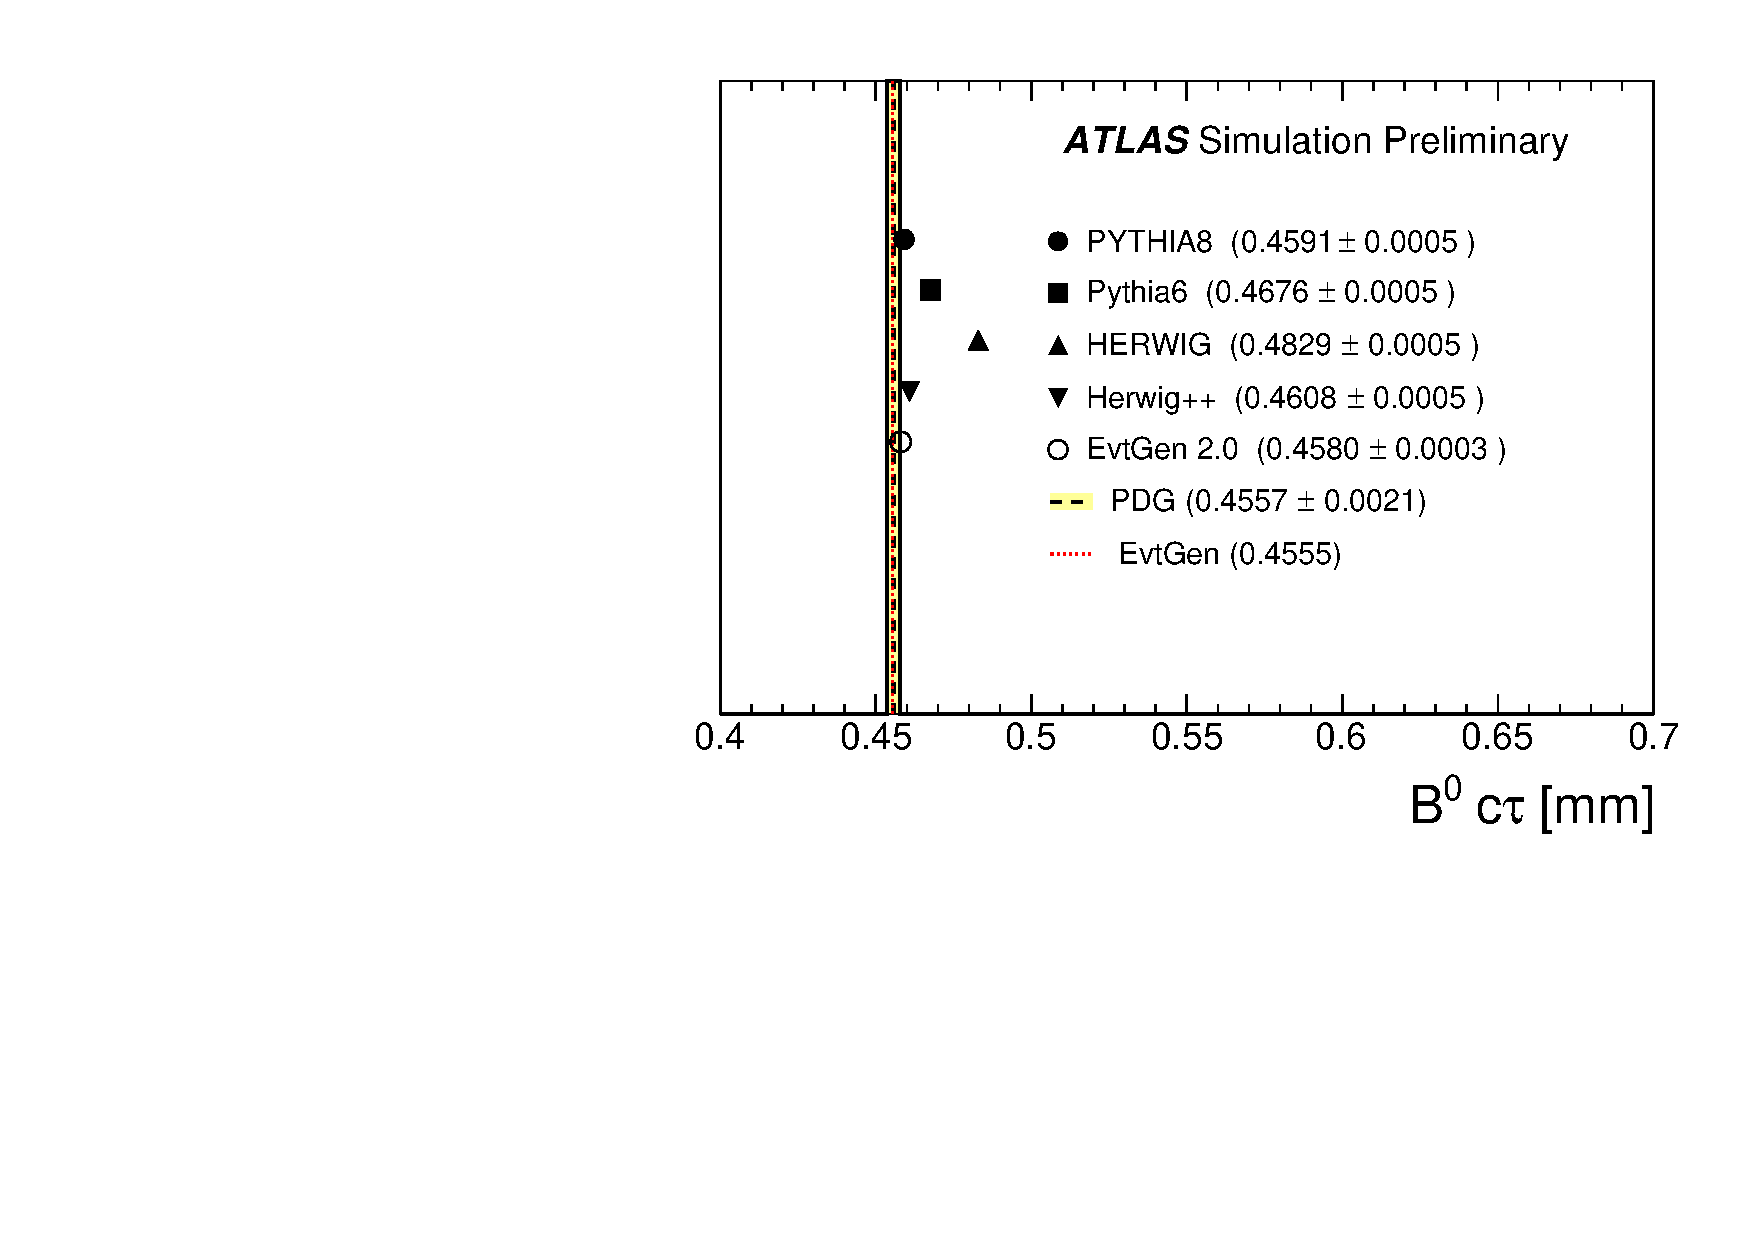
\includegraphics[width=\textwidth]{evtgen/figures/EvtGen/h_B0_life.pdf}
\end{subfigure}
\begin{subfigure}[]{0.45\textwidth}
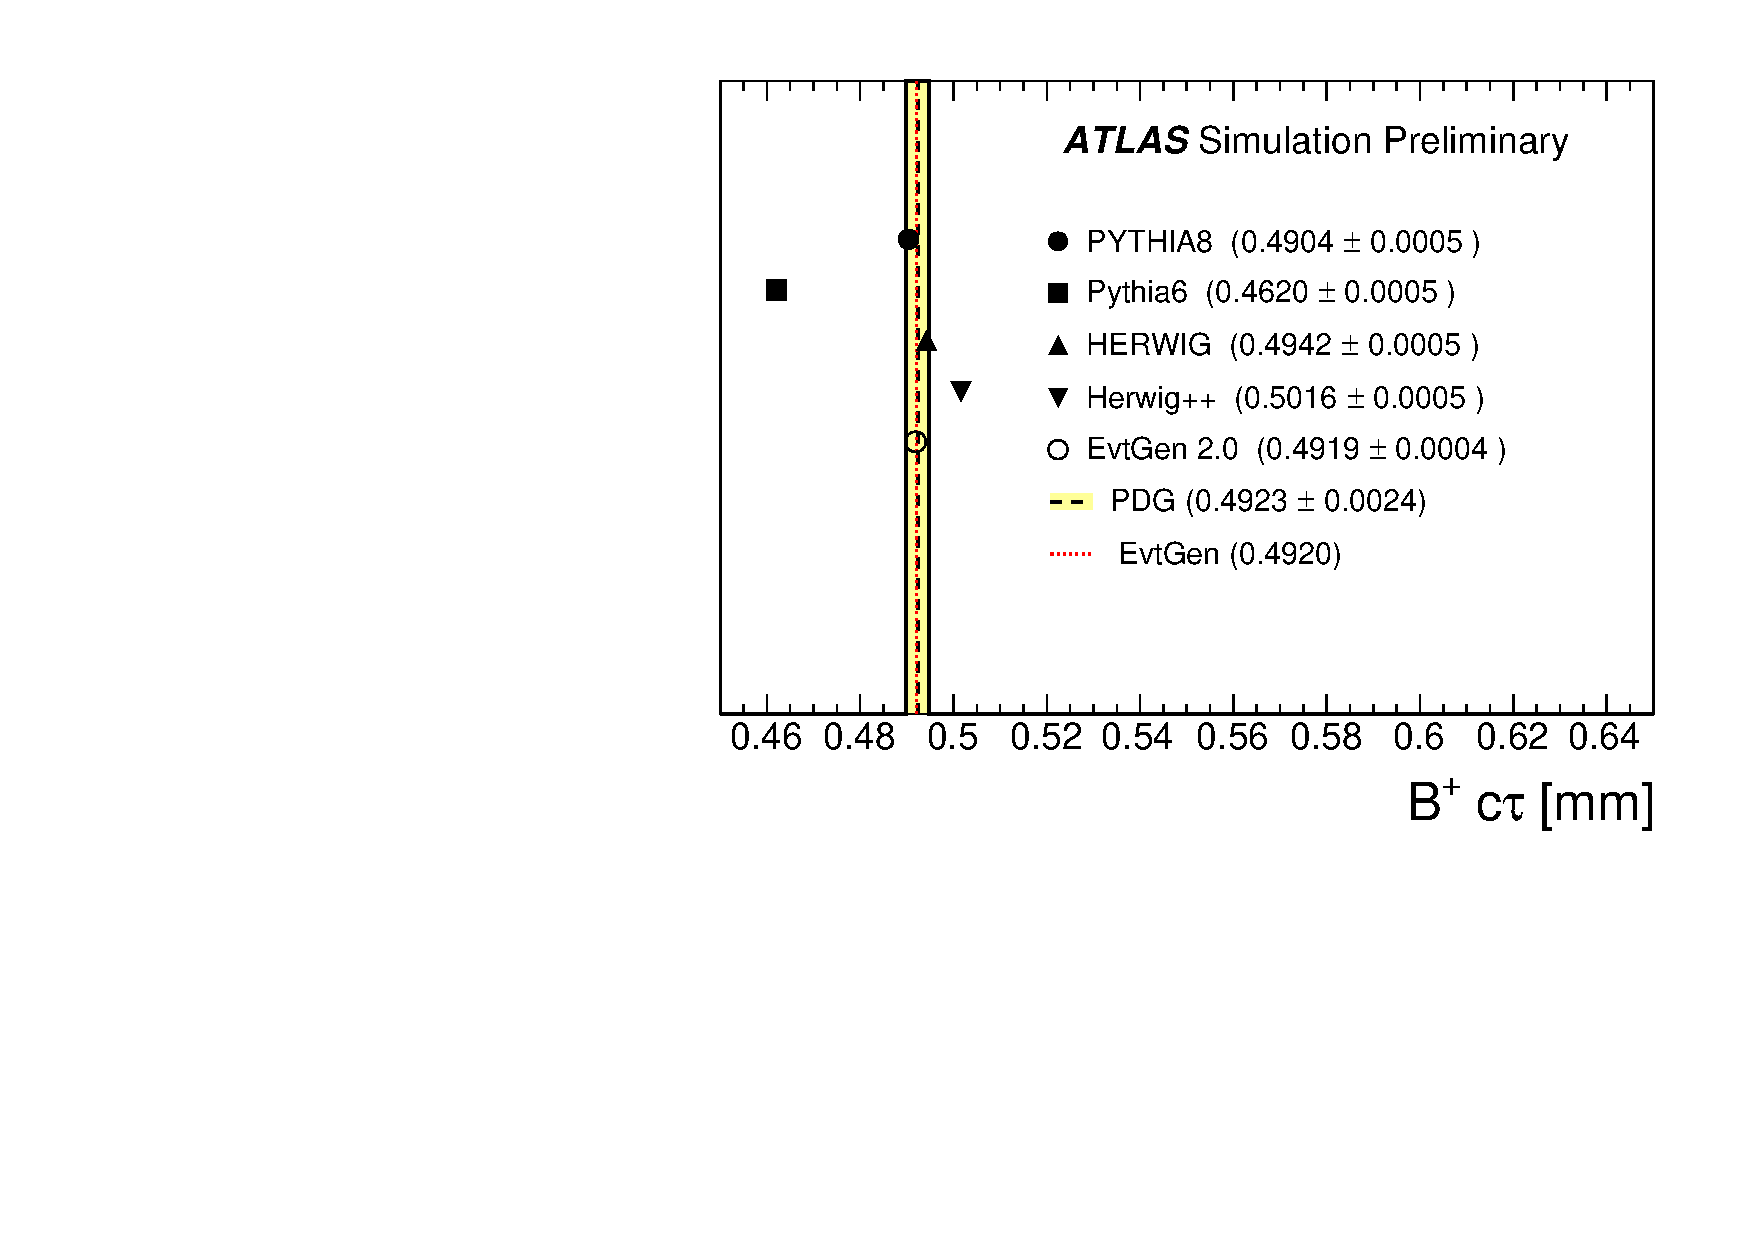
\includegraphics[width=\textwidth]{evtgen/figures/EvtGen/h_B_life.pdf}
\end{subfigure}
\begin{subfigure}[]{0.45\textwidth}
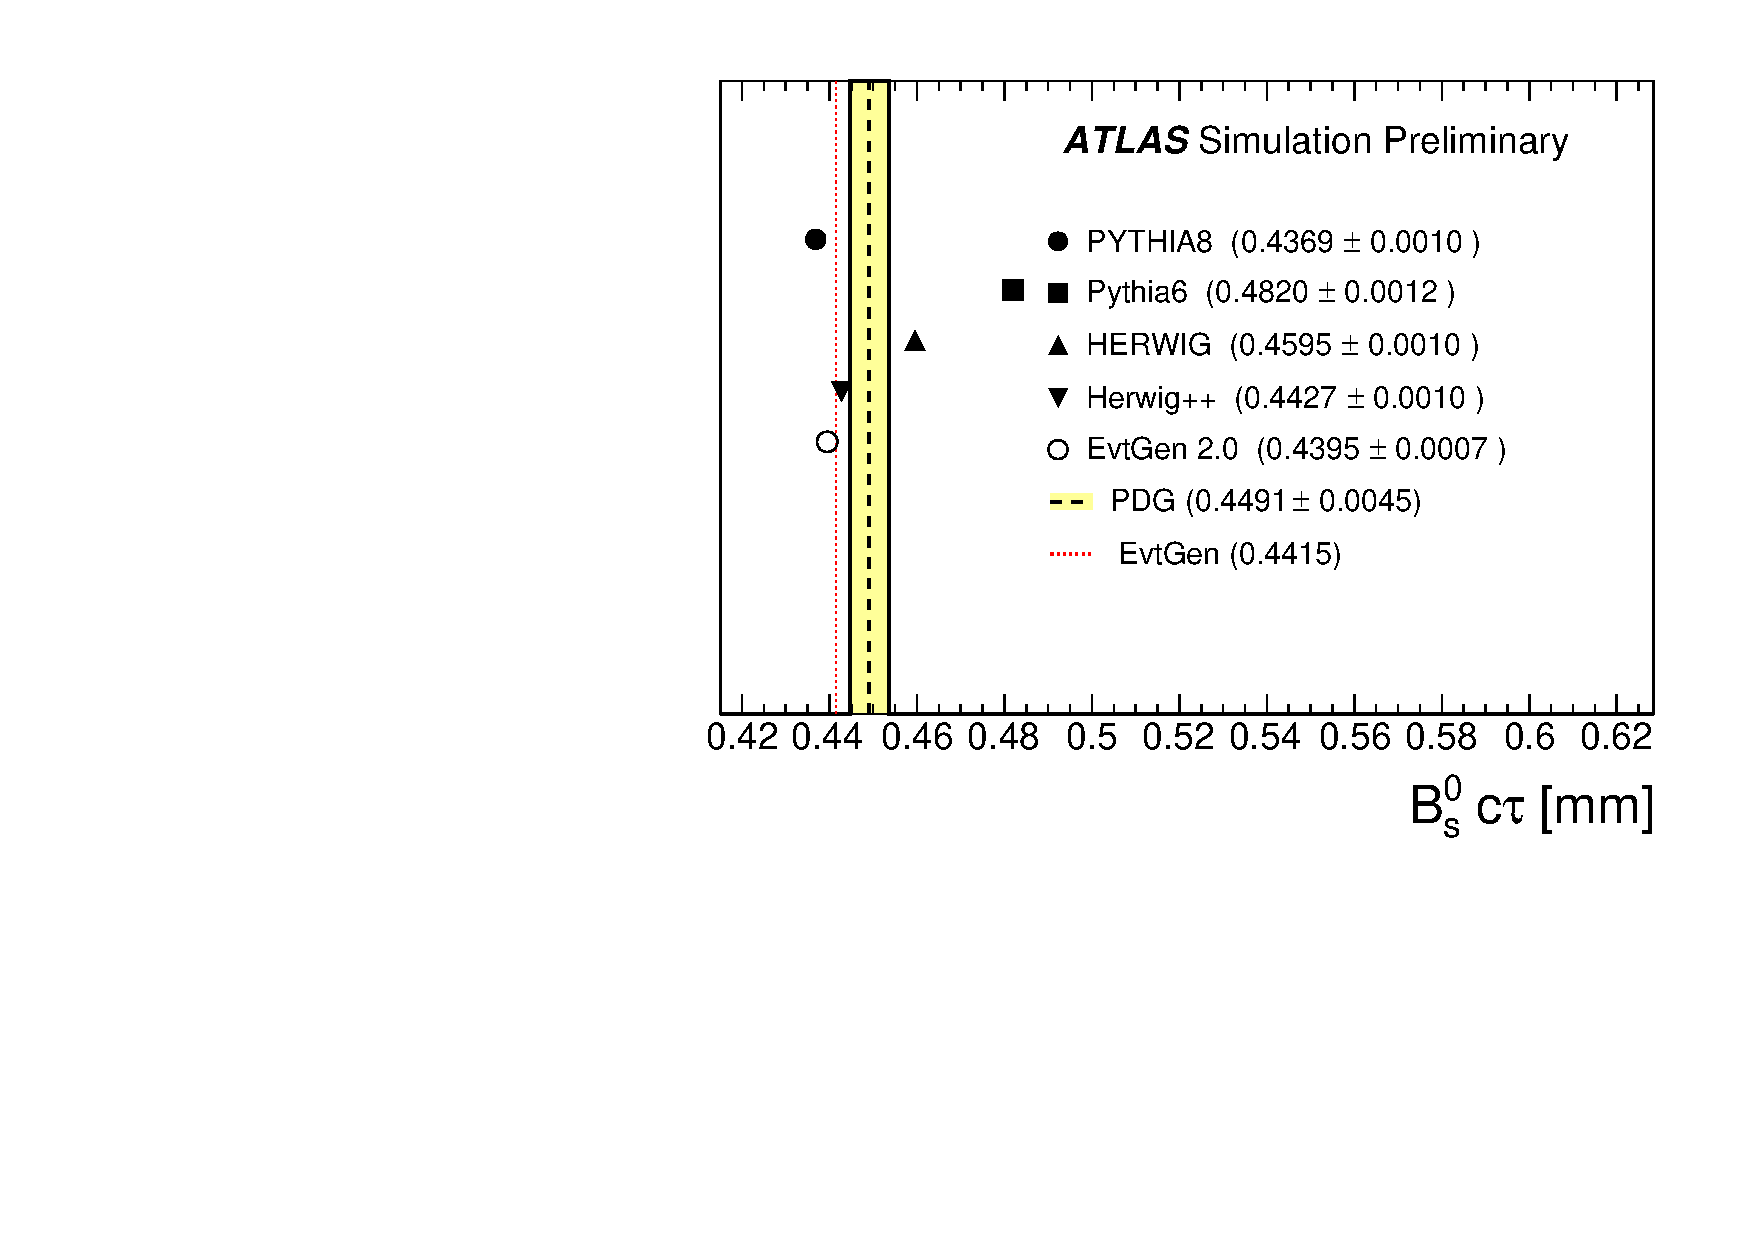
\includegraphics[width=\textwidth]{evtgen/figures/EvtGen/h_Bs_life.pdf}
\end{subfigure}
\begin{subfigure}[]{0.45\textwidth}
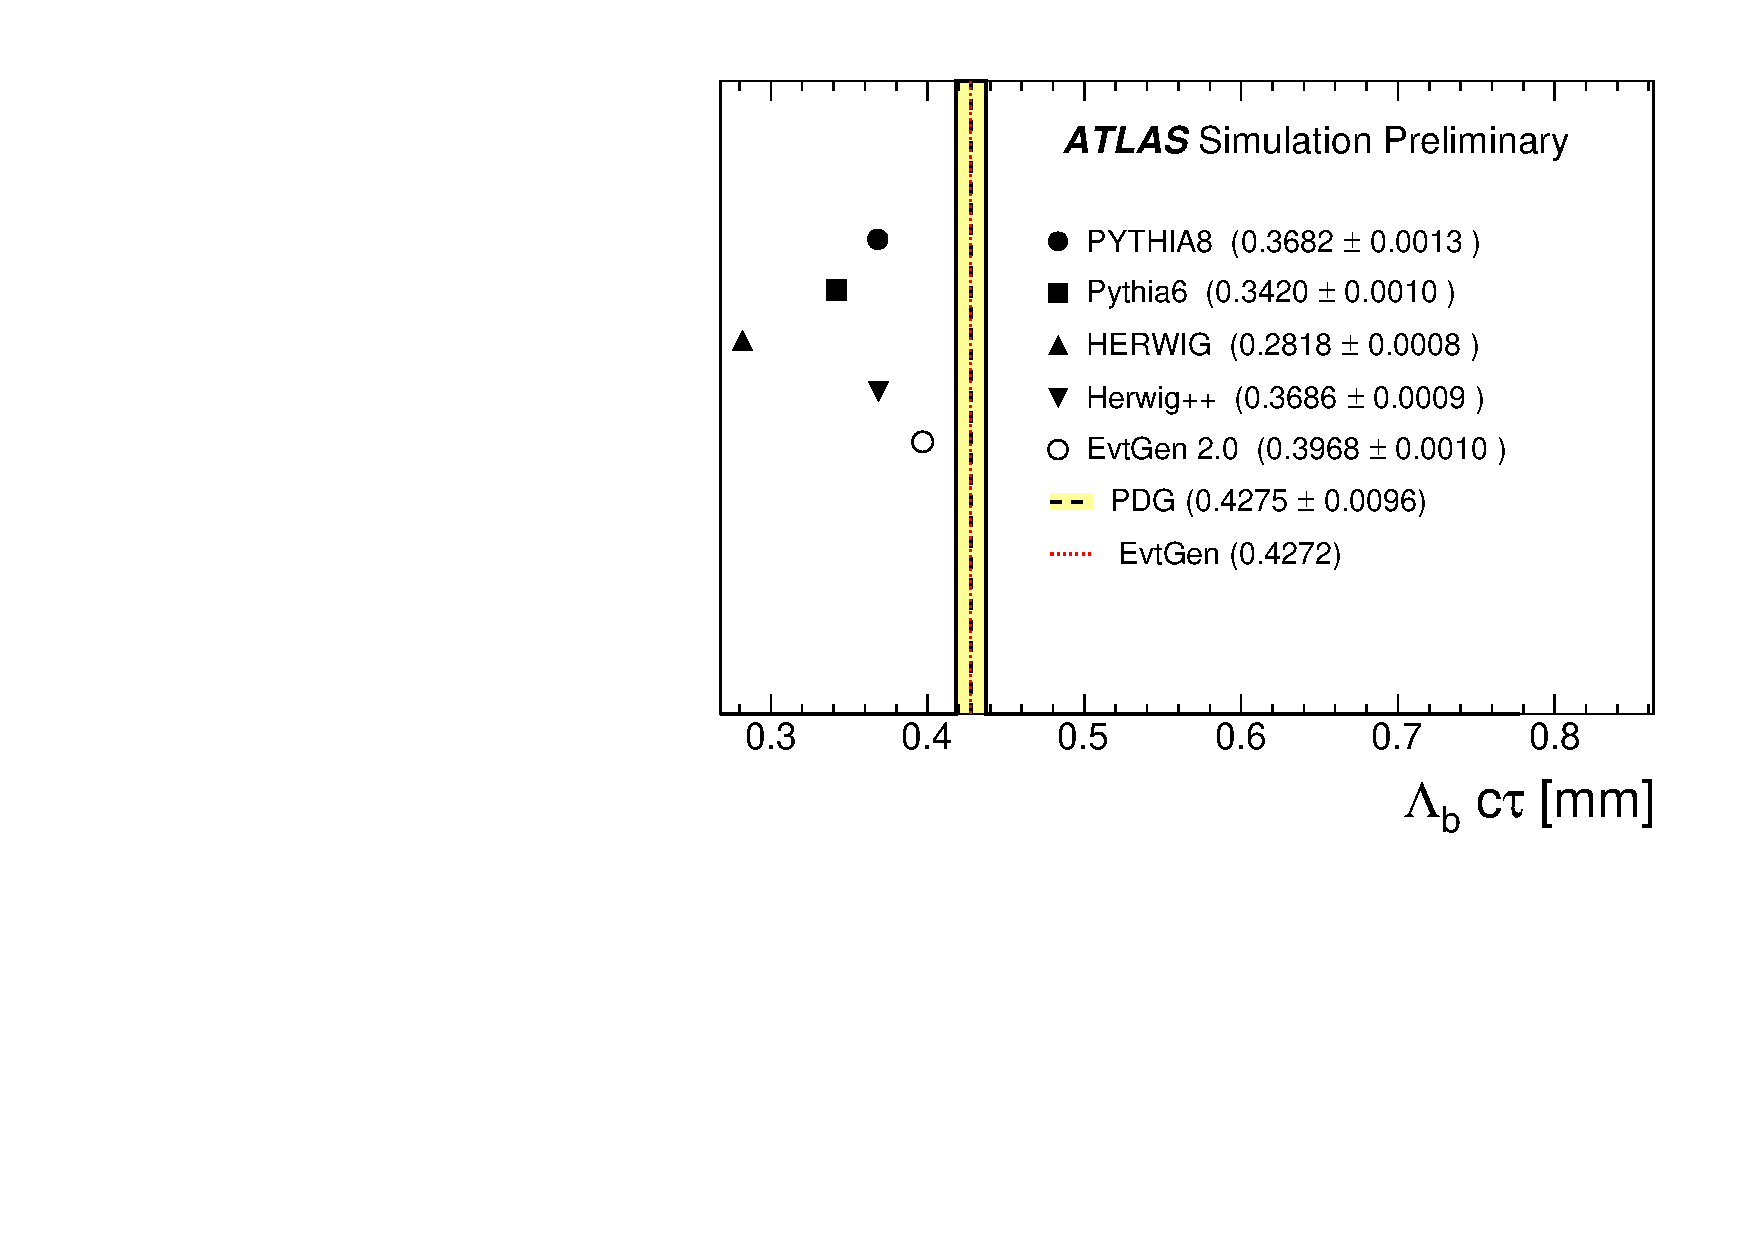
\includegraphics[width=\textwidth]{evtgen/figures/EvtGen/h_Lambdab_life.pdf}
\end{subfigure}
\caption{Comparison of lifetimes of the weakly decaying bottom hadrons 
(a) \Bo,~ (b) \Bp,~ (c) \Bs~ and (d) \Lb~
for four different generators,
\Pythia\ version 427.2, \PythiaE\ version 175, \Herwigpp\  version 2.6.3 and \Herwig\ version 6.520.2, 
both with and without
\EvtGen.  
\EvtGen\ version 2.0 is used with the particle properties table provided with \EvtGen\ and with 
its standard inclusive decay table DECAY\_2010.DEC.
%Adding \EvtGen\ improves agreement of lifetimes with the PDG value. 
The value of the $B_s^0$ lifetime in this default \EvtGen\ particle properties table 
differs from the world average listed by the PDG~\cite{PhysRevD.86.010001}.}
\label{fig:blife}
\end{figure}

\begin{figure}
\centering
\begin{subfigure}[]{0.45\textwidth}
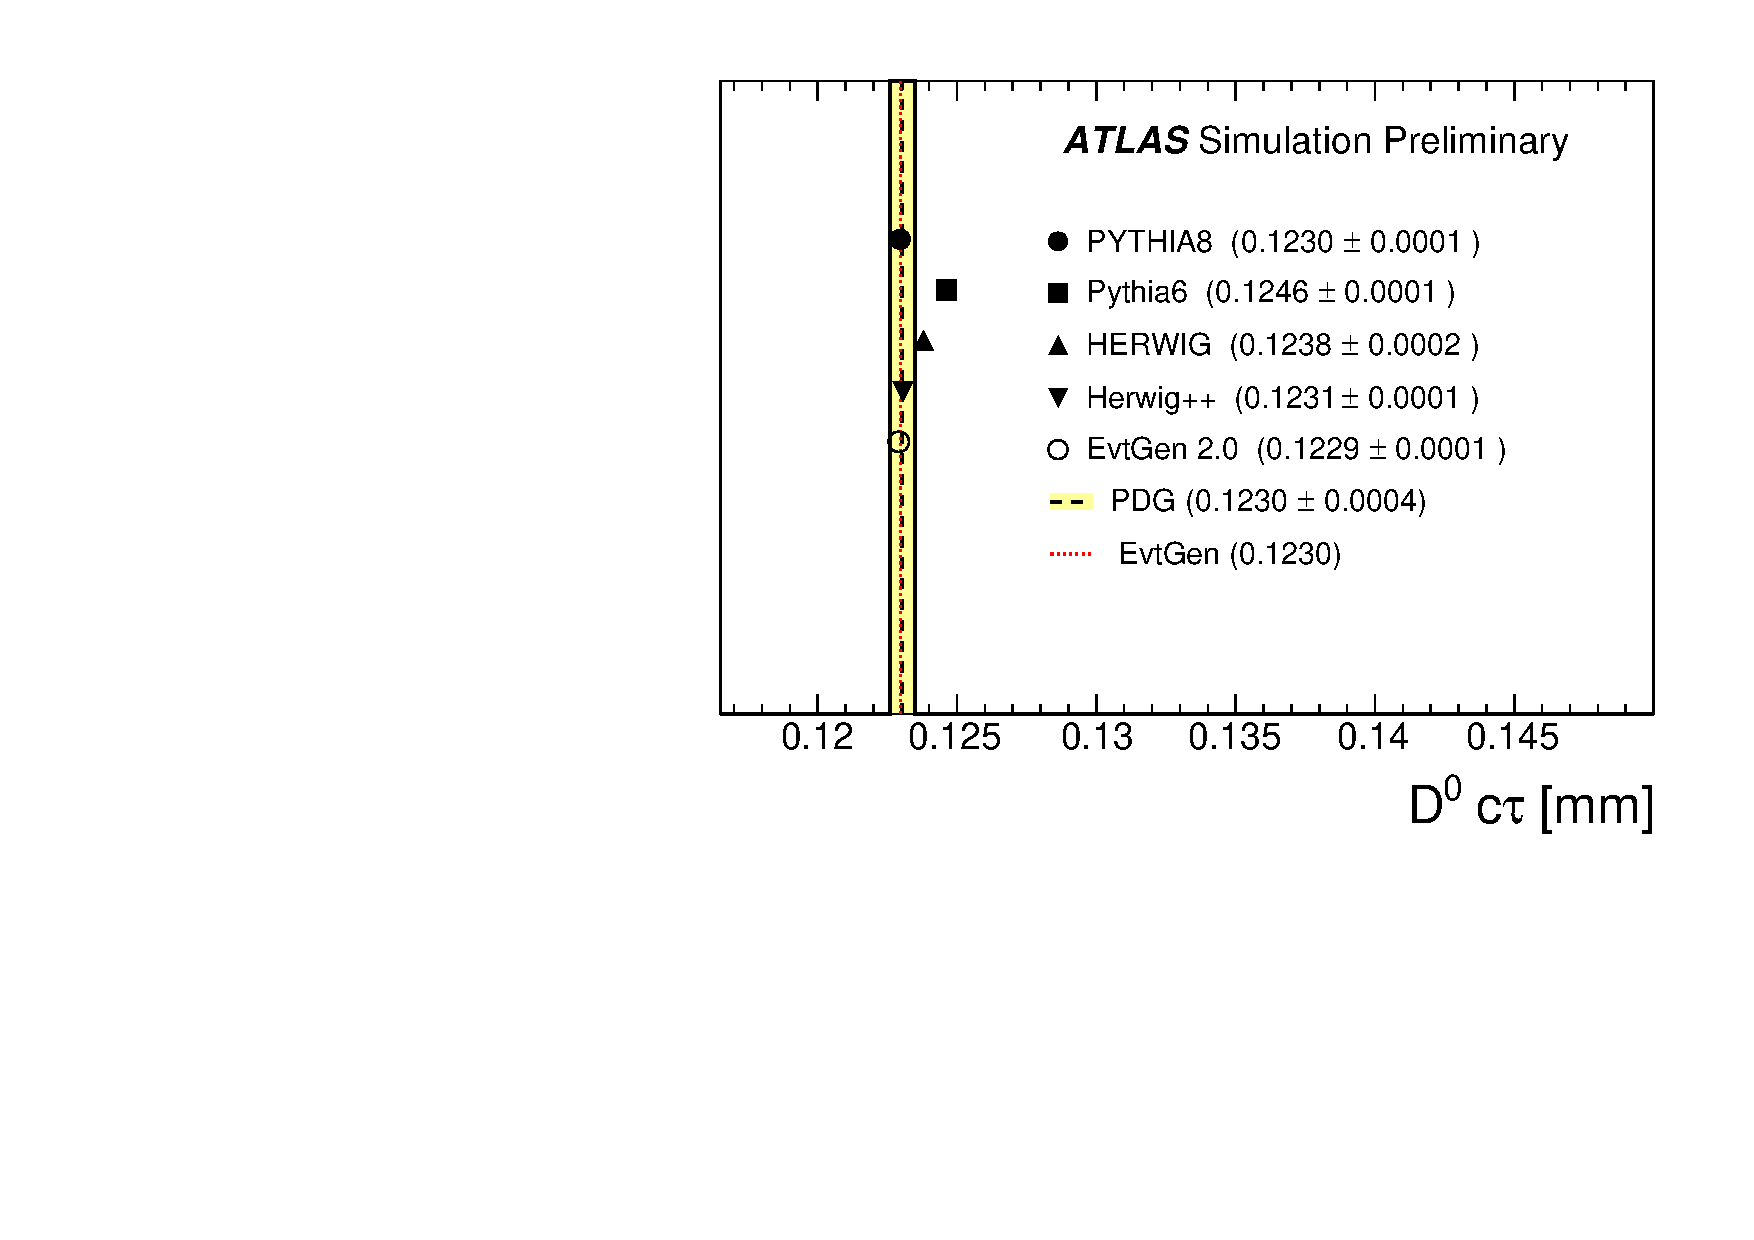
\includegraphics[width=\textwidth]{evtgen/figures/EvtGen/h_D0_life.pdf}
\end{subfigure}
\begin{subfigure}[]{0.45\textwidth}
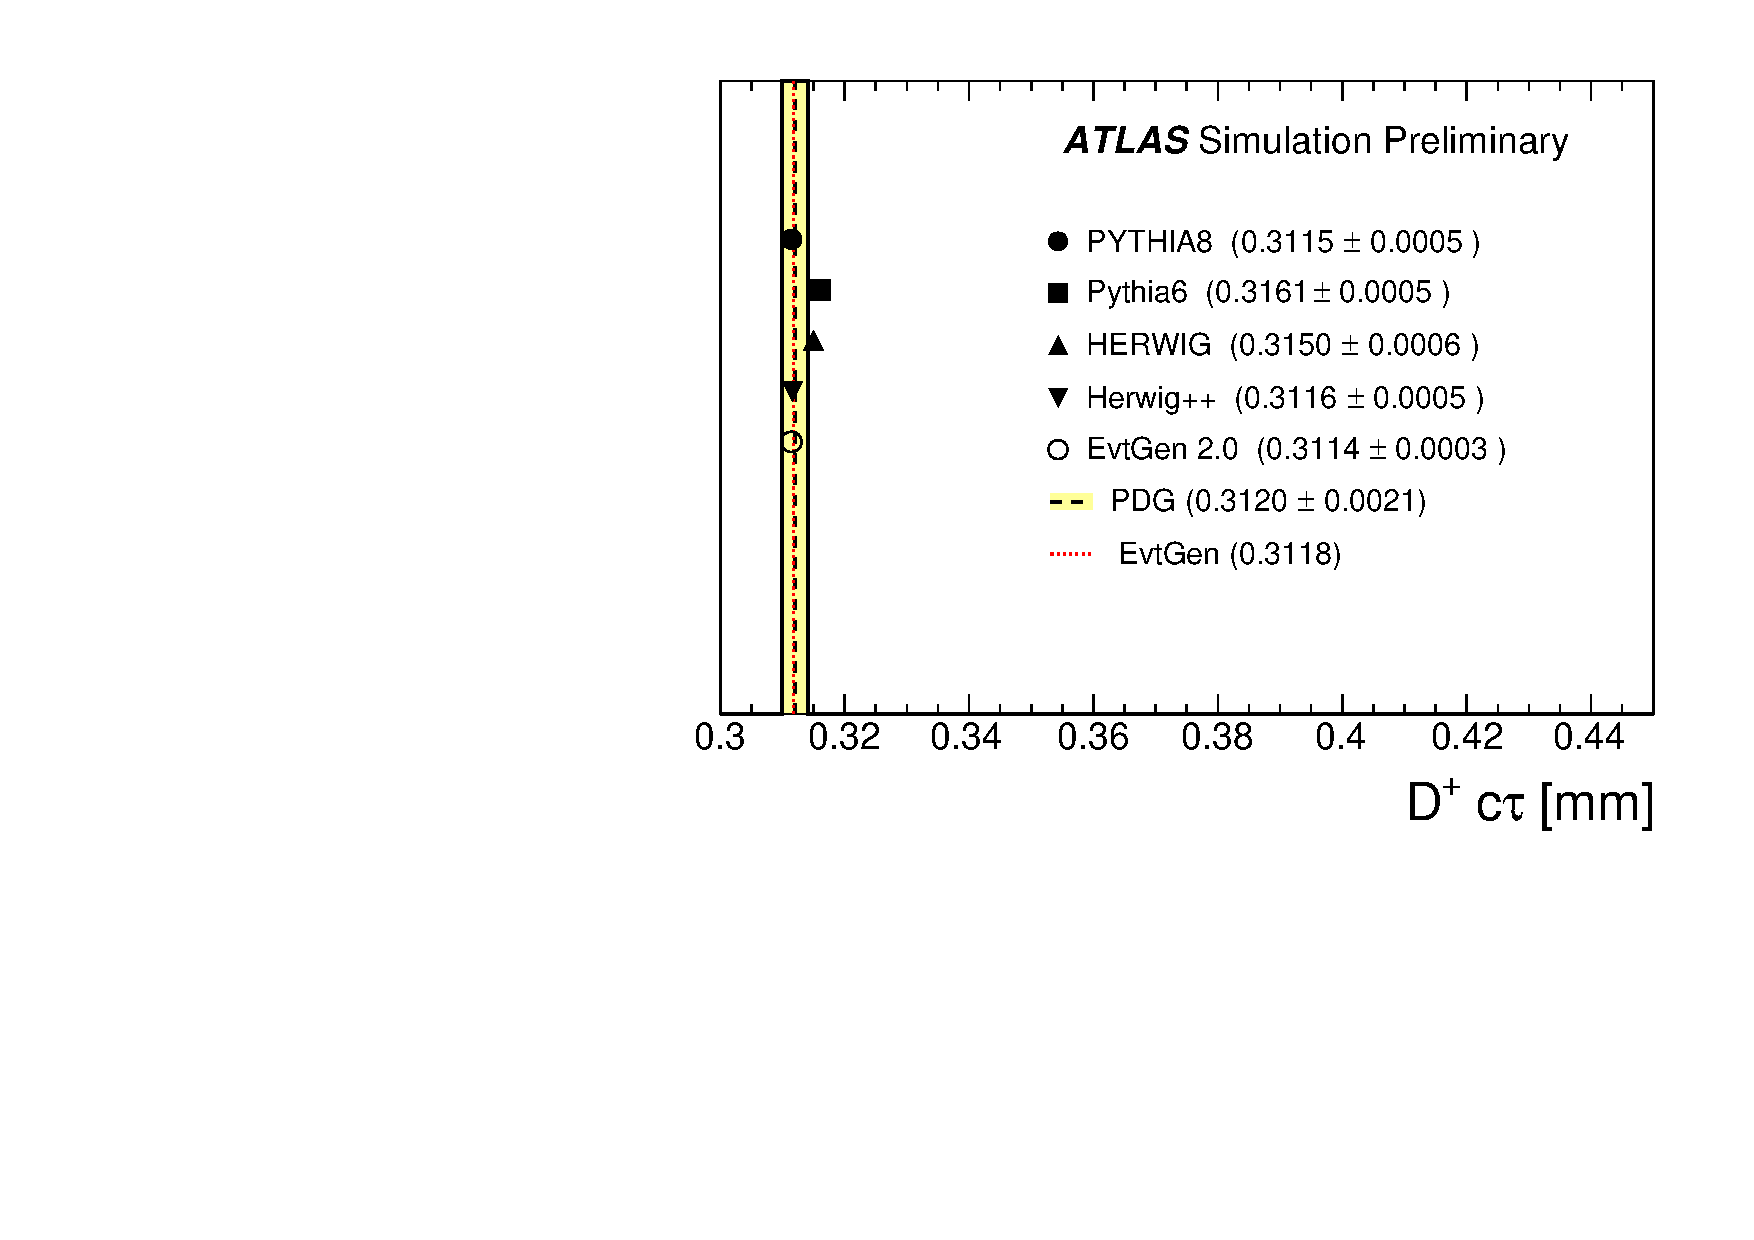
\includegraphics[width=\textwidth]{evtgen/figures/EvtGen/h_D_life.pdf}
\end{subfigure}\\
\begin{subfigure}[]{0.45\textwidth}
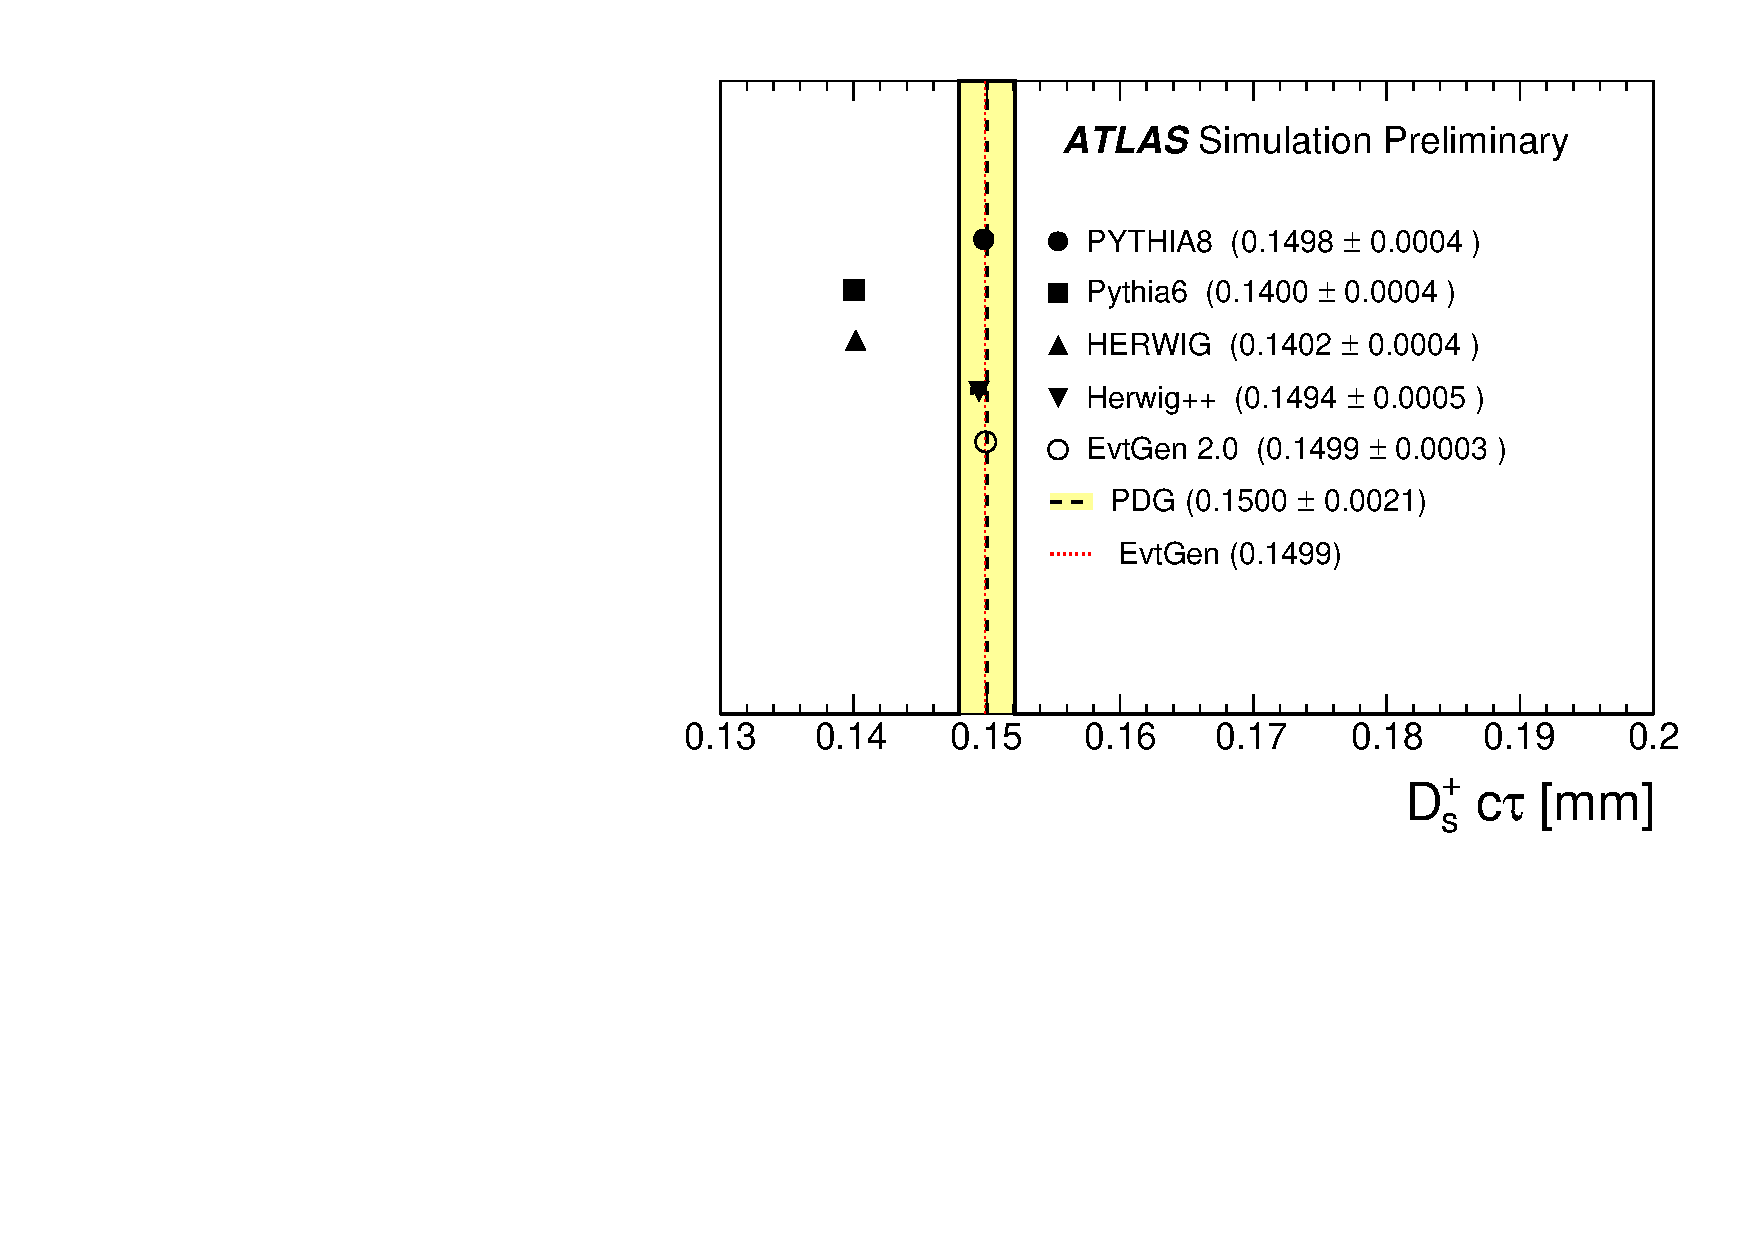
\includegraphics[width=\textwidth]{evtgen/figures/EvtGen/h_Ds_life.pdf}
\end{subfigure}
\begin{subfigure}[]{0.45\textwidth}
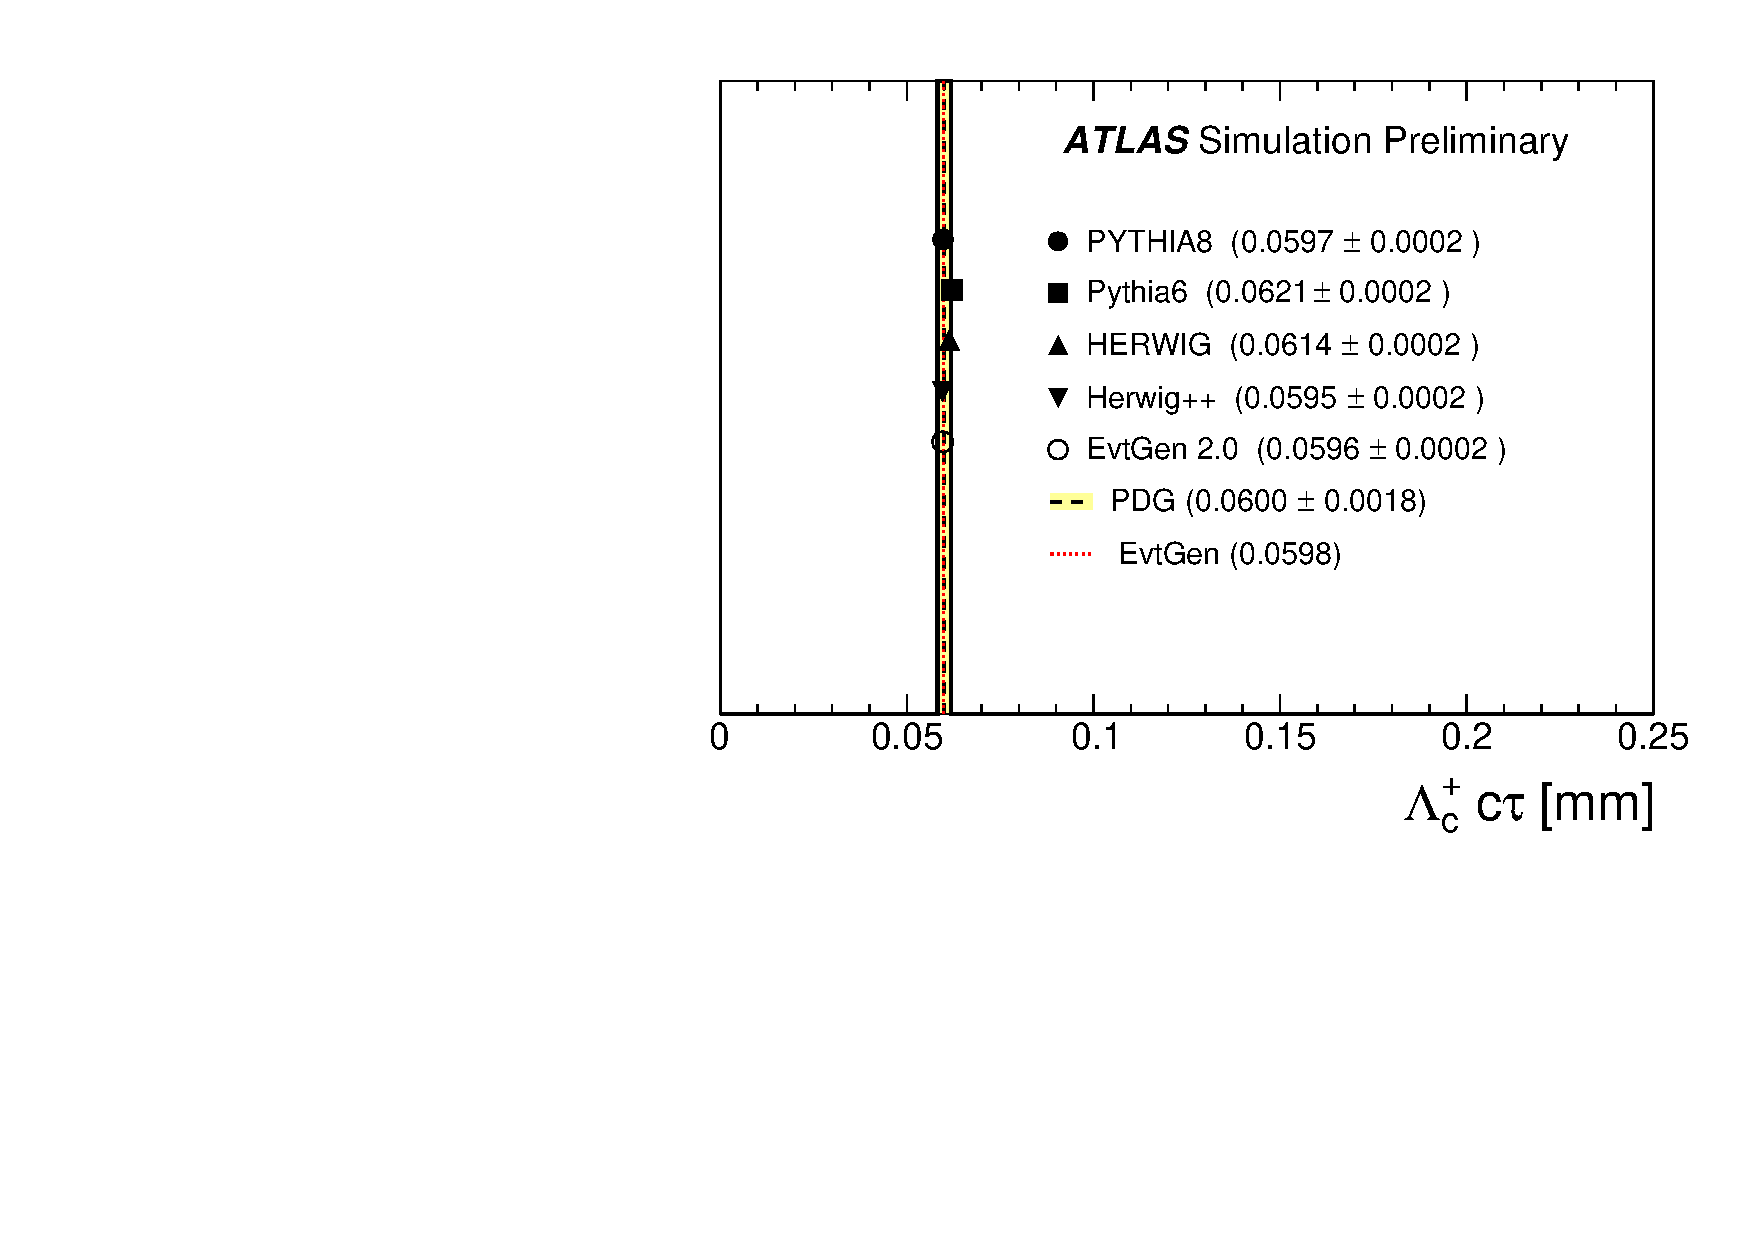
\includegraphics[width=\textwidth]{evtgen/figures/EvtGen/h_Lambdac_life.pdf}
\end{subfigure}
\caption{Comparison of lifetimes of the weakly decaying charm hadrons 
(a) \Dzero, (b) \Dplus, (c) \Ds\ and (d) \Lc~
in four different generators,
\Pythia\ version 427.2, \PythiaE\ version 175, \Herwigpp\  version 2.6.3 and \Herwig\ version 6.520.2, 
both with and without
\EvtGen.  
\EvtGen\ version 2.0 is used with the particle properties table provided with \EvtGen\ and with 
its standard inclusive decay table DECAY\_2010.DEC.
}
\label{fig:clife}
\end{figure}


\begin{figure}
\centering
\begin{subfigure}[]{0.45\textwidth}
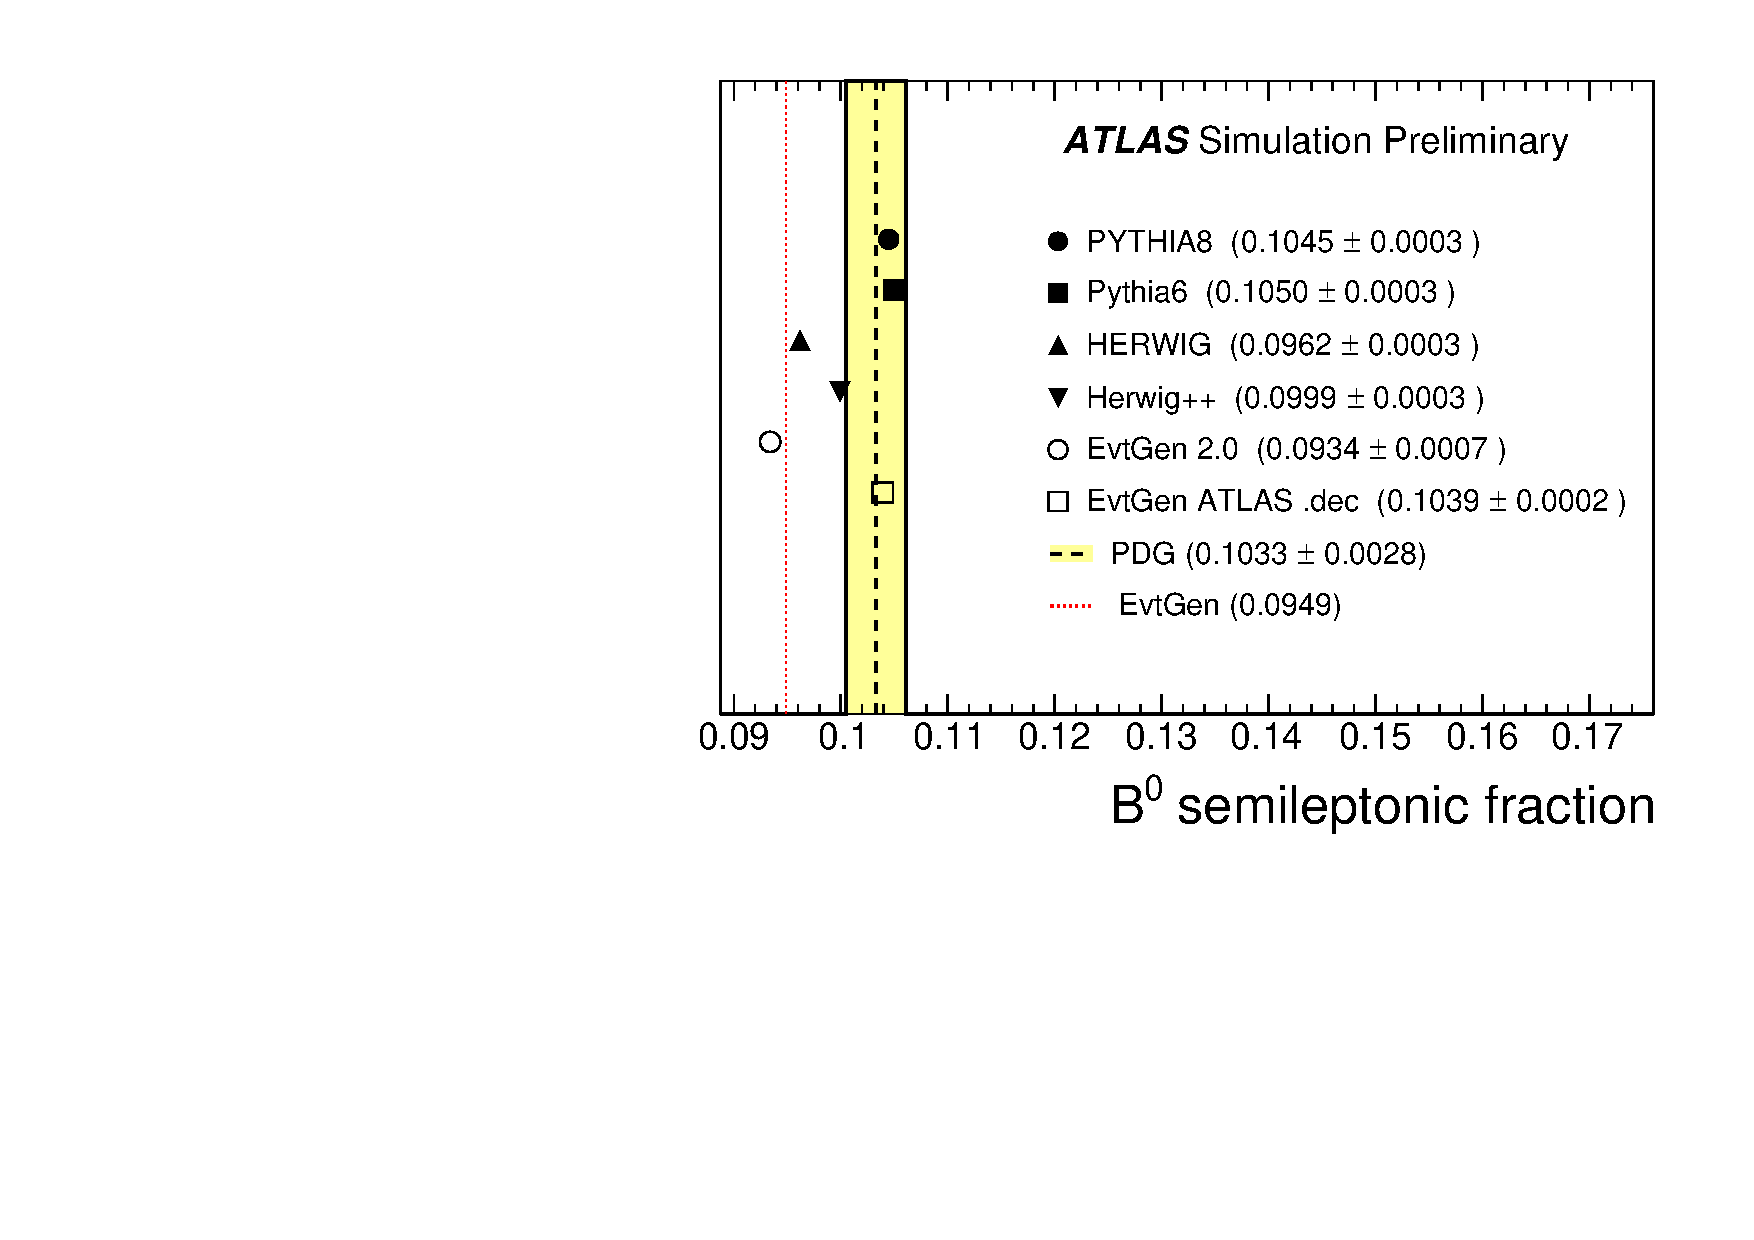
\includegraphics[width=\textwidth]{evtgen/figures/EvtGen/h_B0_sl.pdf}
\end{subfigure}
\begin{subfigure}[]{0.45\textwidth}
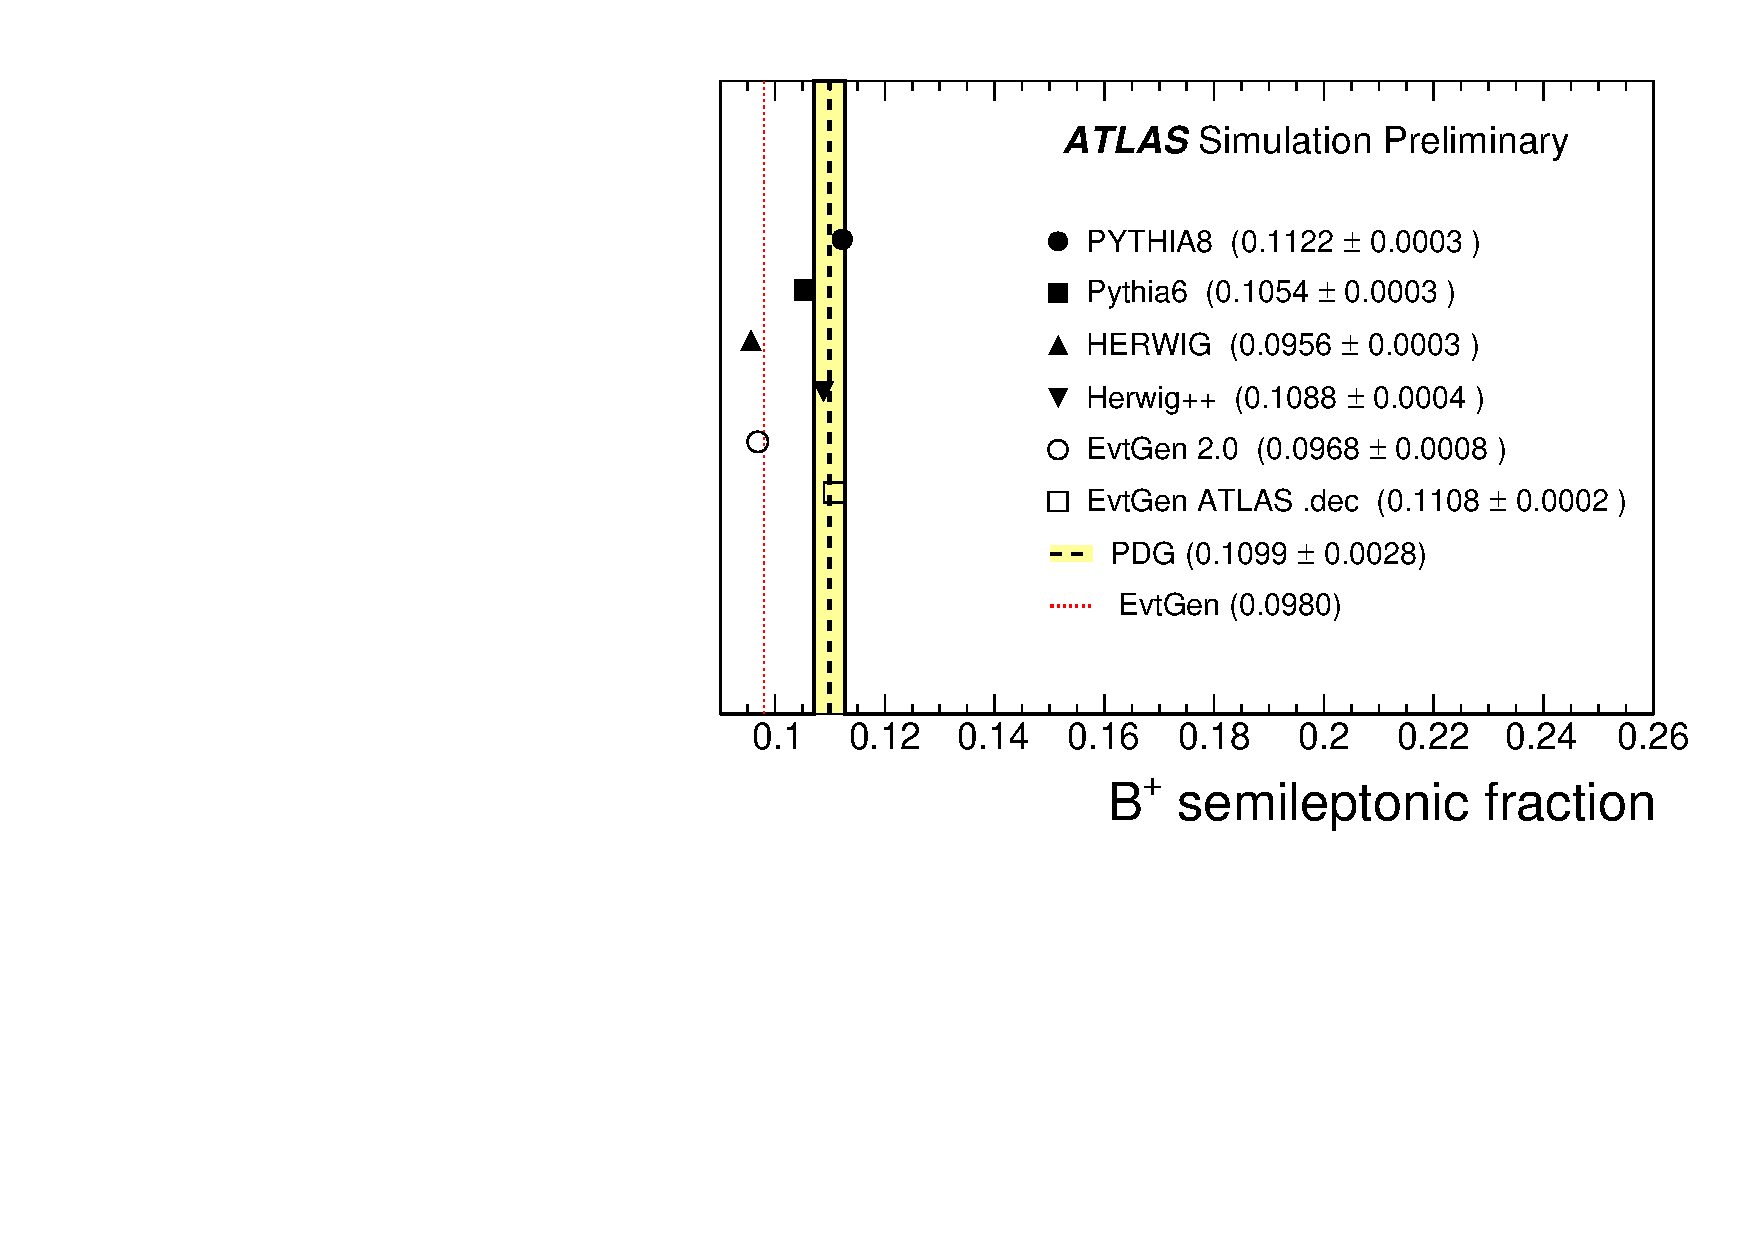
\includegraphics[width=\textwidth]{evtgen/figures/EvtGen/h_B_sl.pdf}
\end{subfigure}
\begin{subfigure}[]{0.45\textwidth}
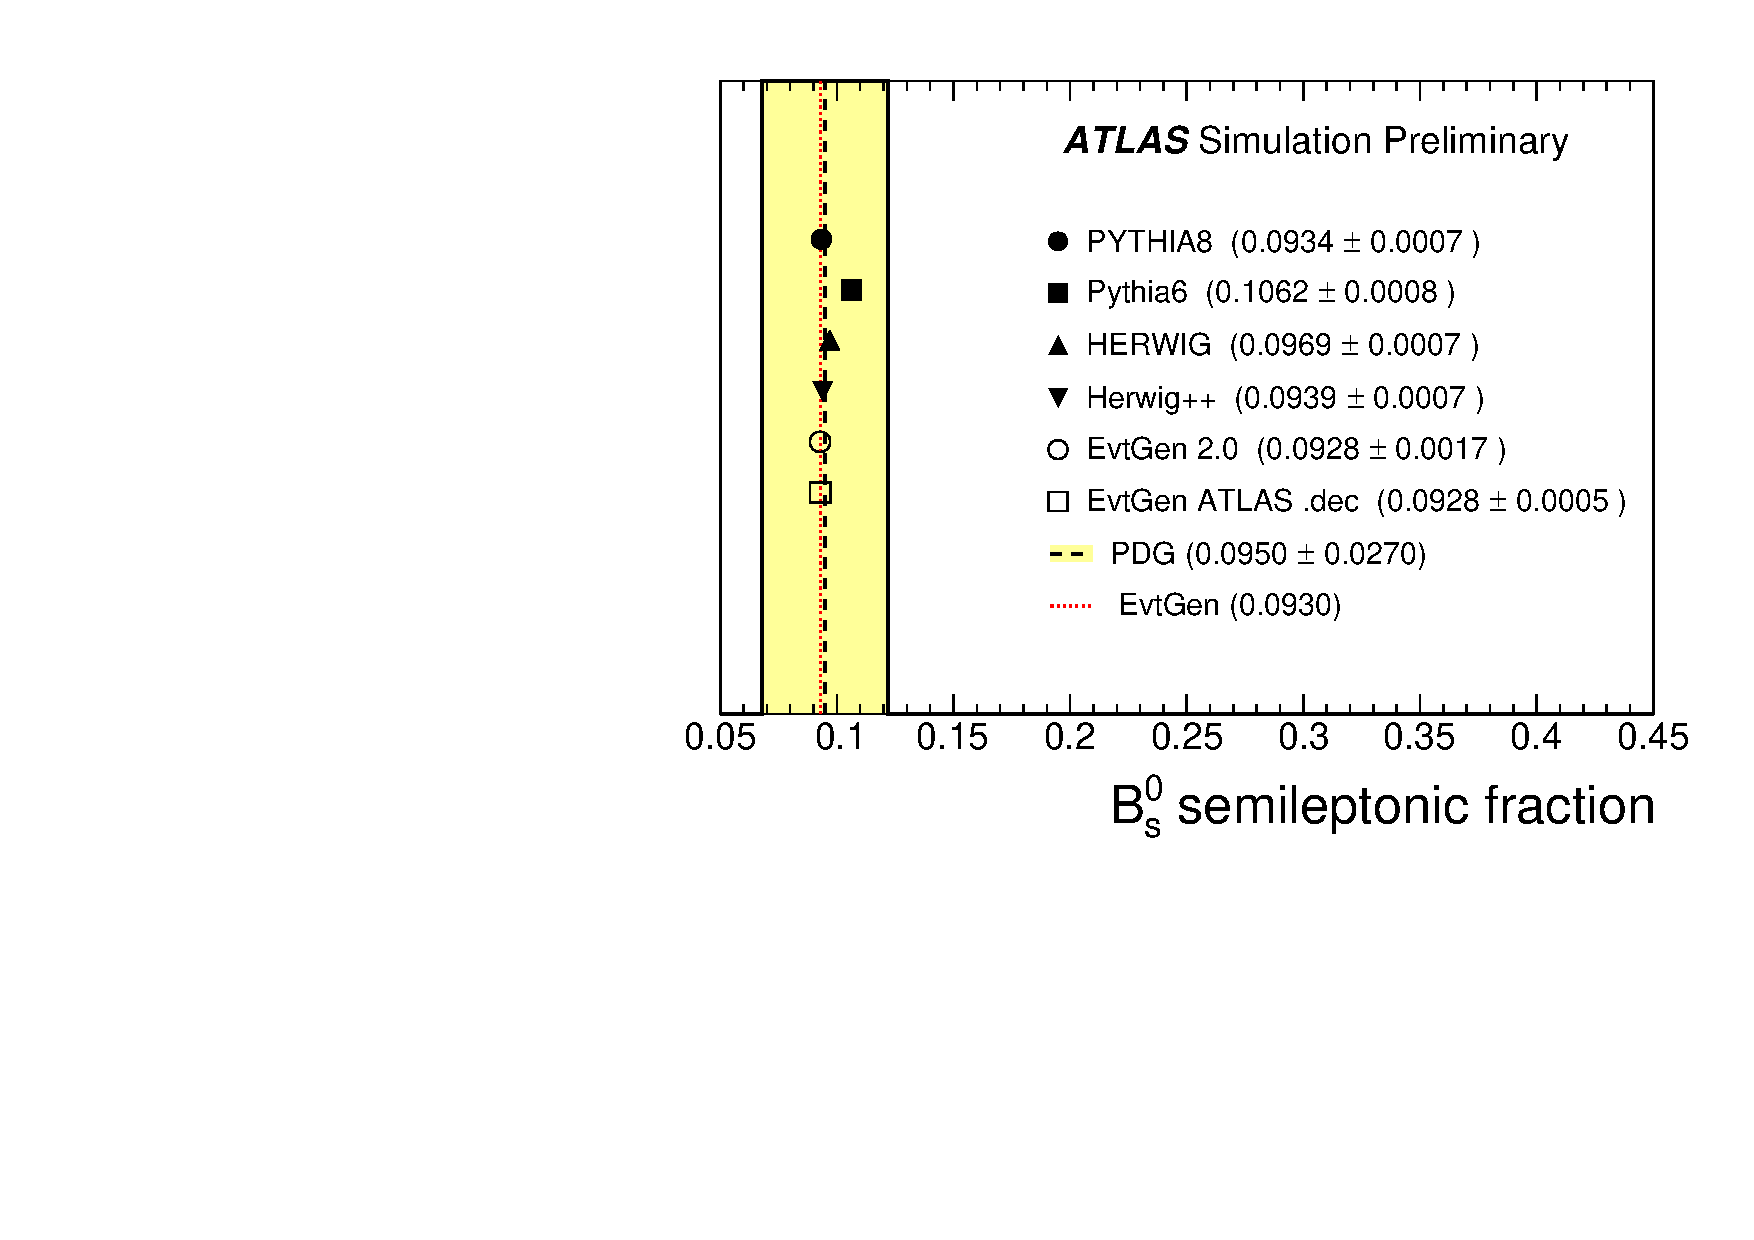
\includegraphics[width=\textwidth]{evtgen/figures/EvtGen/h_Bs_sl.pdf}
\end{subfigure}
\begin{subfigure}[]{0.45\textwidth}
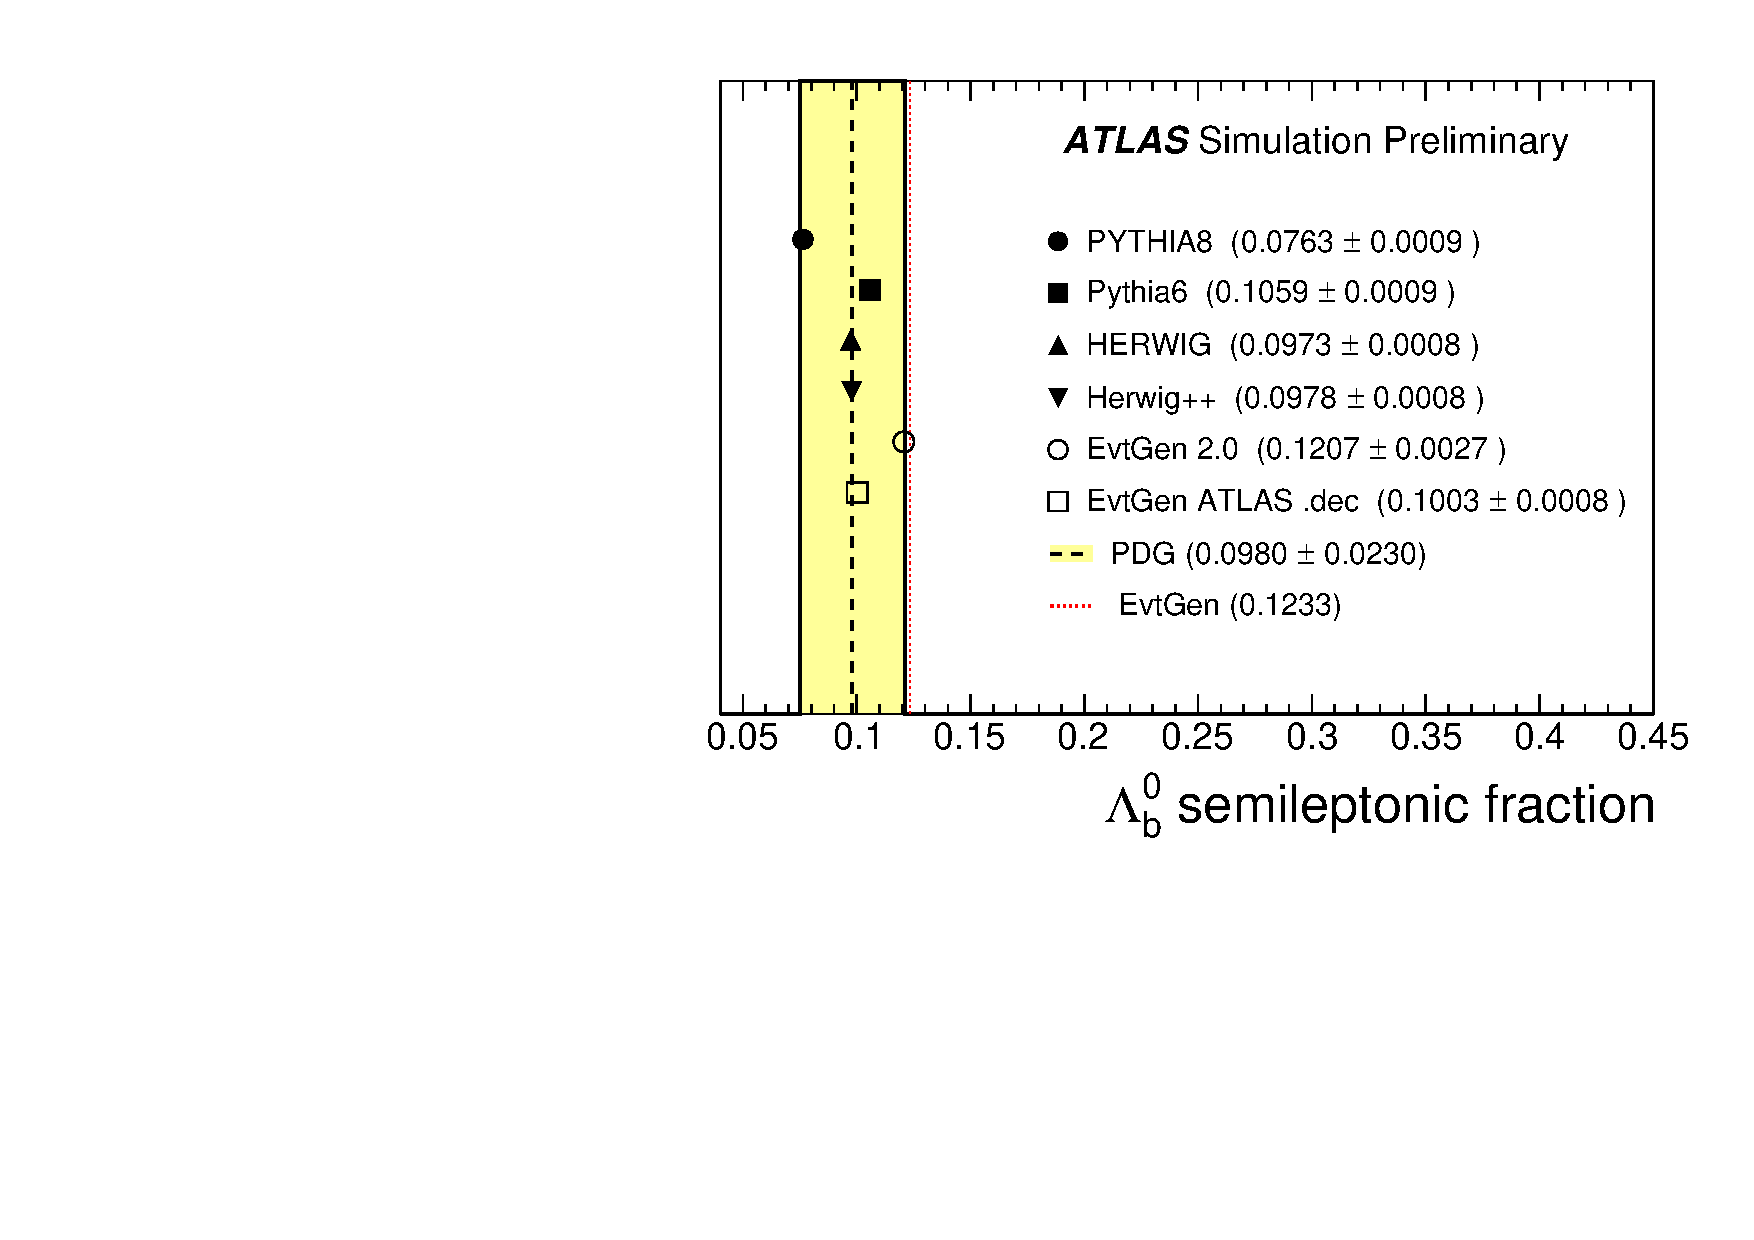
\includegraphics[width=\textwidth]{evtgen/figures/EvtGen/h_Lambdab_sl.pdf}
\end{subfigure}
\caption{Comparison of semileptonic branching fraction $B\rightarrow e^-\overline{\nu_e} X$ 
of the weakly decaying bottom hadrons 
(a) \Bo, (b) \Bp, (c) \Bs~ and (d) \Lb~
in four different generators,
%Adding \EvtGen\ improves agreement with the PDG value. 
\Pythia\ version 427.2, \PythiaE\ version 175, \Herwigpp\  version 2.6.3 and \Herwig\ version 6.520.2, 
both with and without
\EvtGen.  
\EvtGen\ version 2.0 is used with the particle properties table provided with \EvtGen\ and with 
its standard inclusive decay table DECAY\_2010.DEC, as well as a custom decay table with developed for ATLAS with the most up to date semileptonic fractions from the PDG.
Only decays where the electron is the direct decay product of the bottom hadron are included here (e.g.
electrons coming from charm or $\tau $ decays are excluded).
The band shown for the world average branching fractions correspond to the
measured decay fraction for $B\rightarrow e\nu X_c$ listed by the PDG\cite{PhysRevD.86.010001}.
The values of the $B^0$, $B^+$ and $\Lambda^0_b$~semileptonic fractions in the 
default \EvtGen\ particle properties table have been tuned to the
observed inclusive $B\rightarrow D\ell\nu+\mathrm{anything}$ branching fraction, which has a 
larger uncertainty.}
\label{fig:bsl}
\end{figure}

\begin{figure}
\centering
\begin{subfigure}[]{0.45\textwidth}
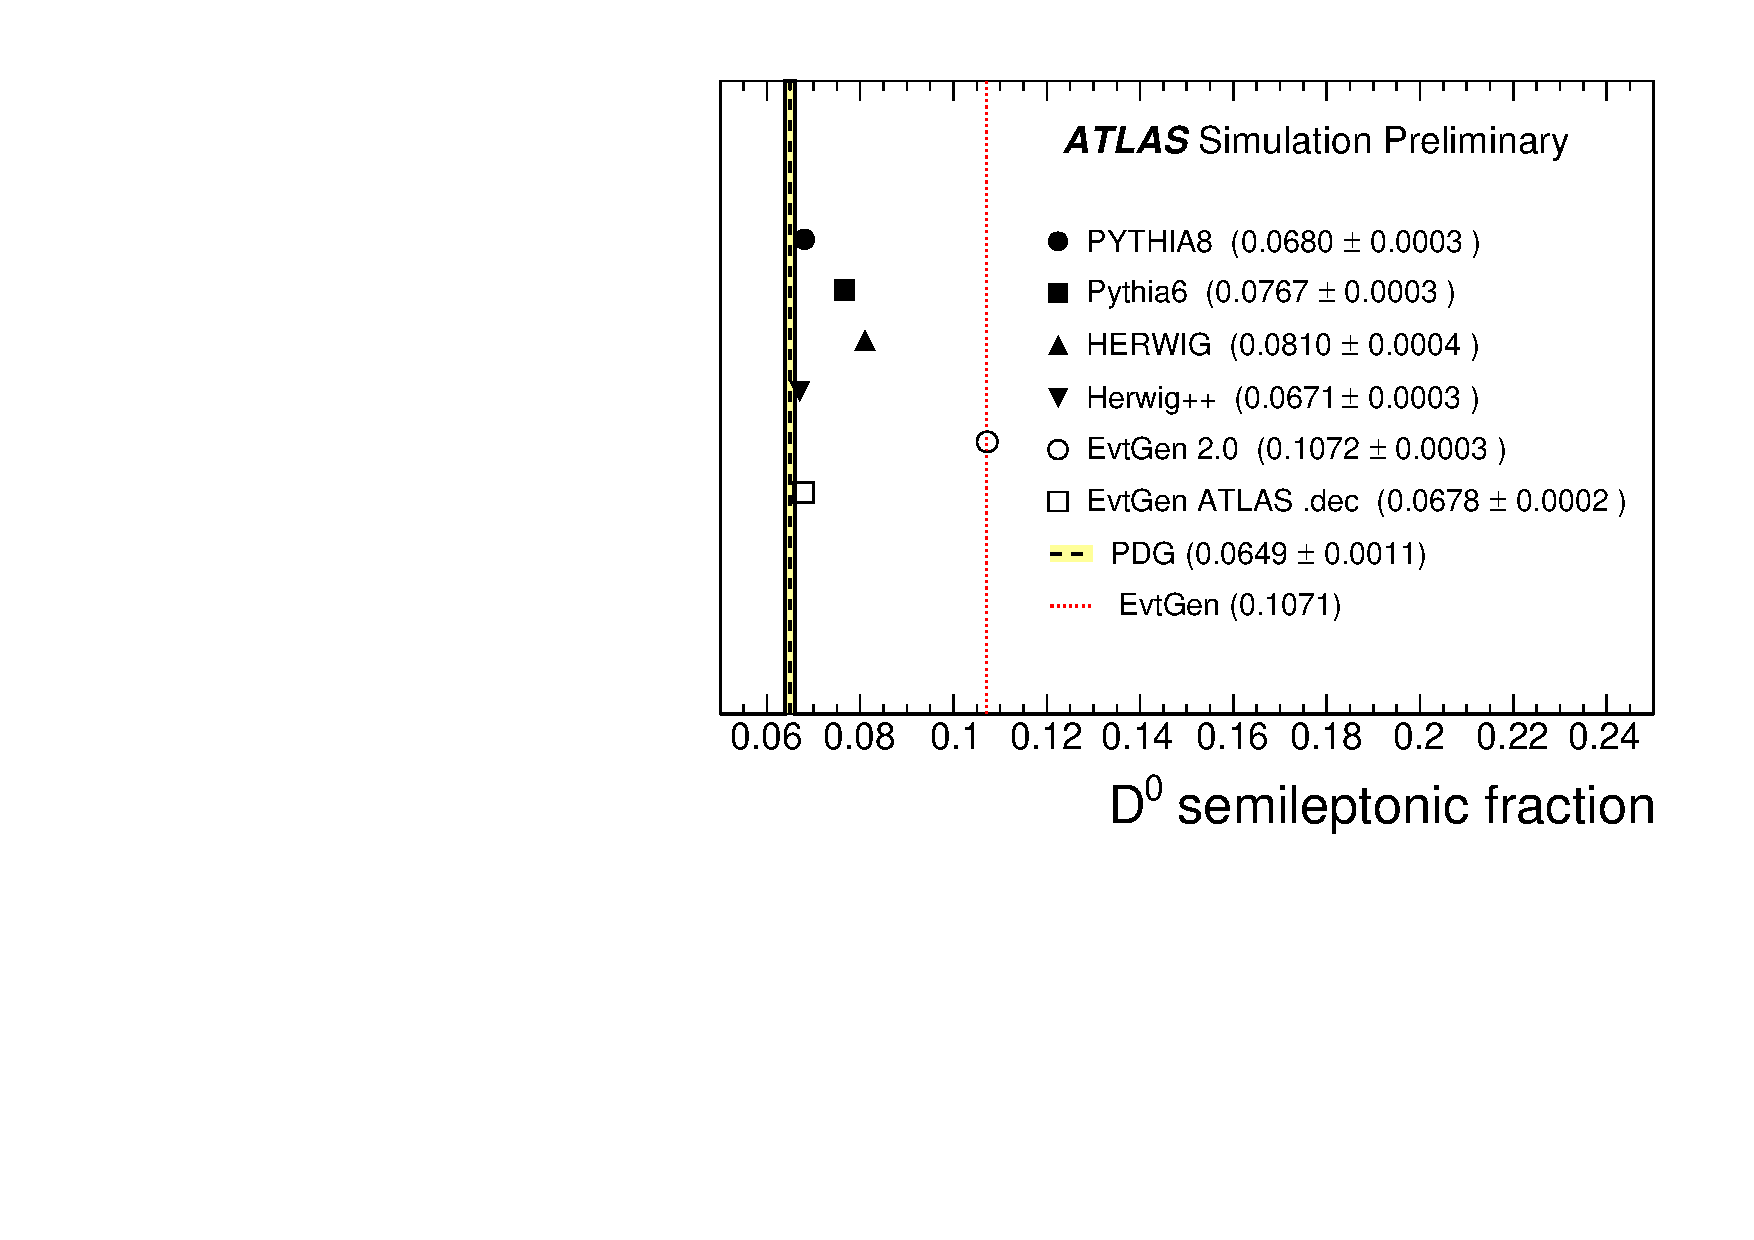
\includegraphics[width=\textwidth]{evtgen/figures/EvtGen/h_D0_sl.pdf}
\end{subfigure}
\begin{subfigure}[]{0.45\textwidth}
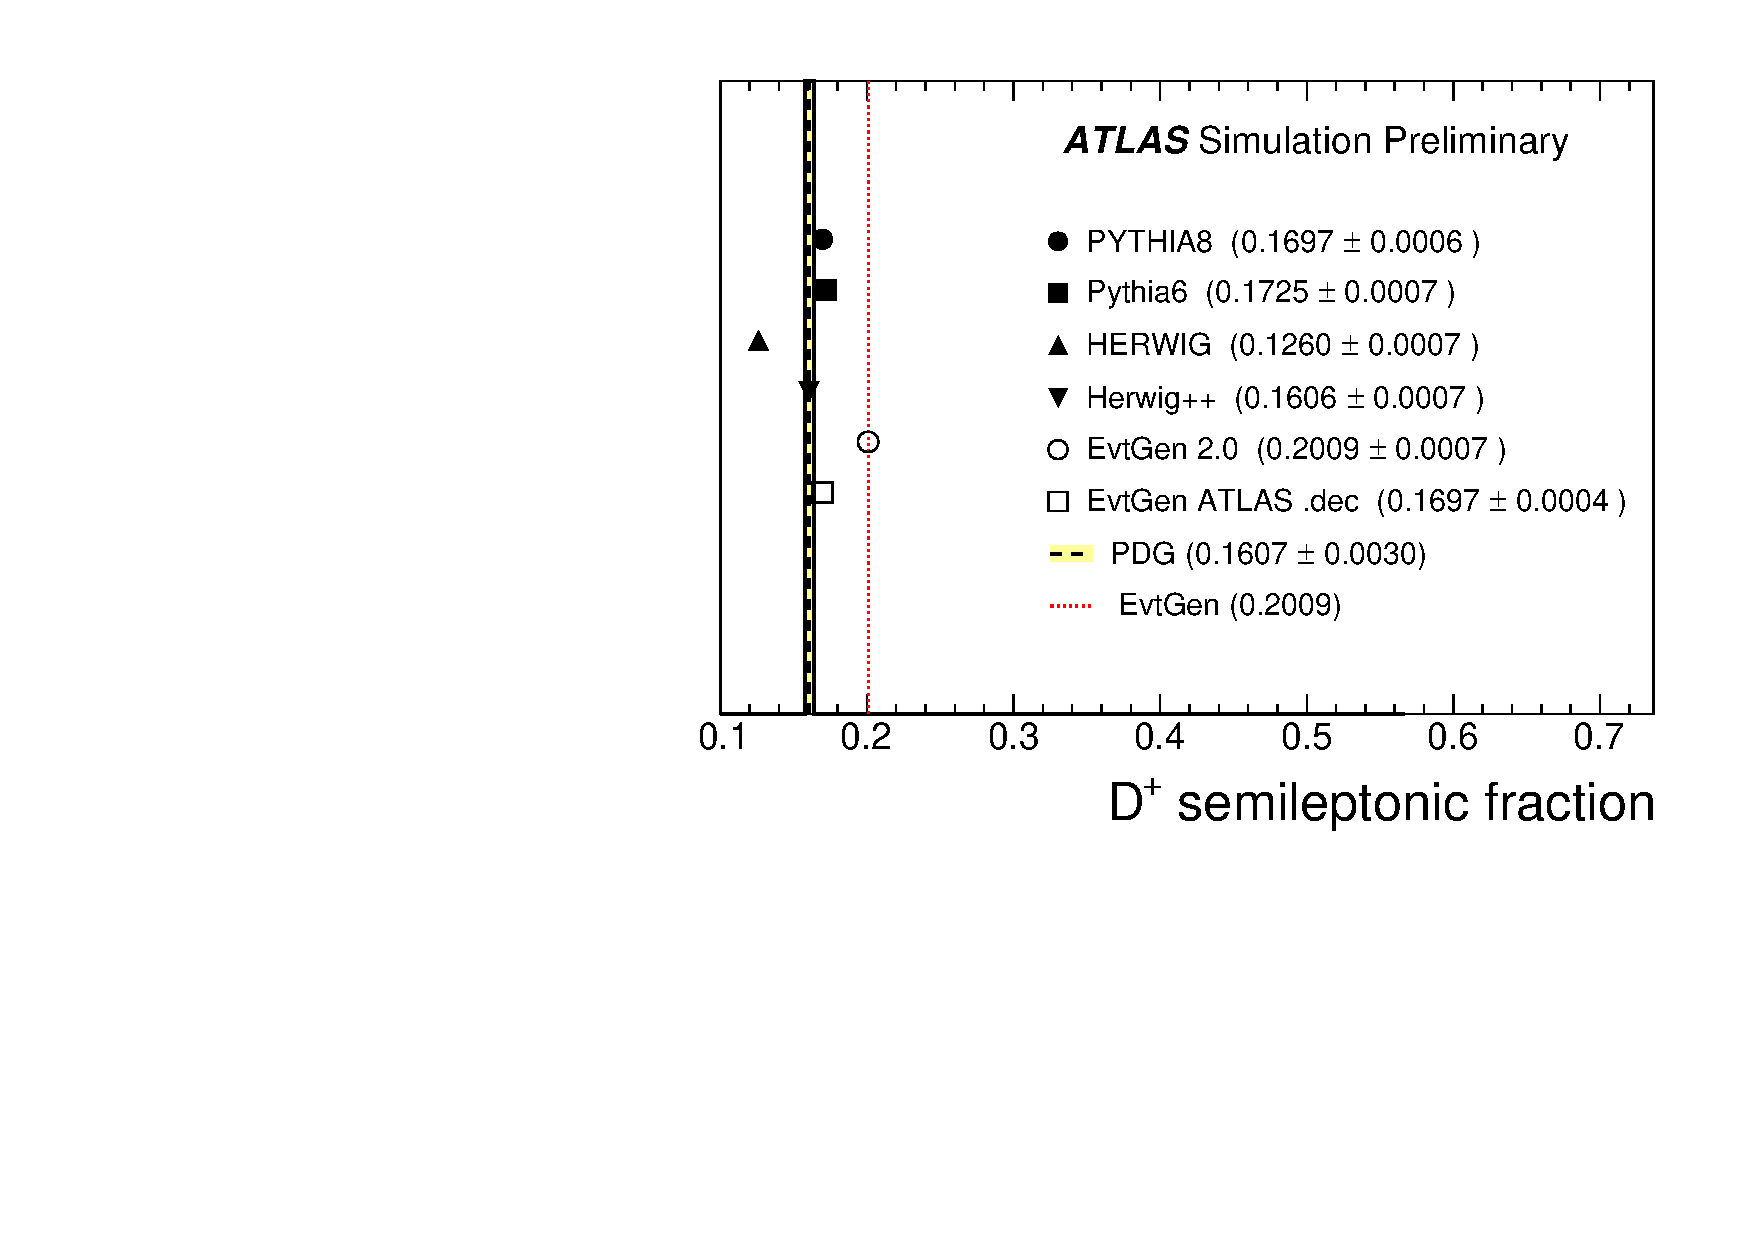
\includegraphics[width=\textwidth]{evtgen/figures/EvtGen/h_D_sl.pdf}
\end{subfigure}
\begin{subfigure}[]{0.45\textwidth}
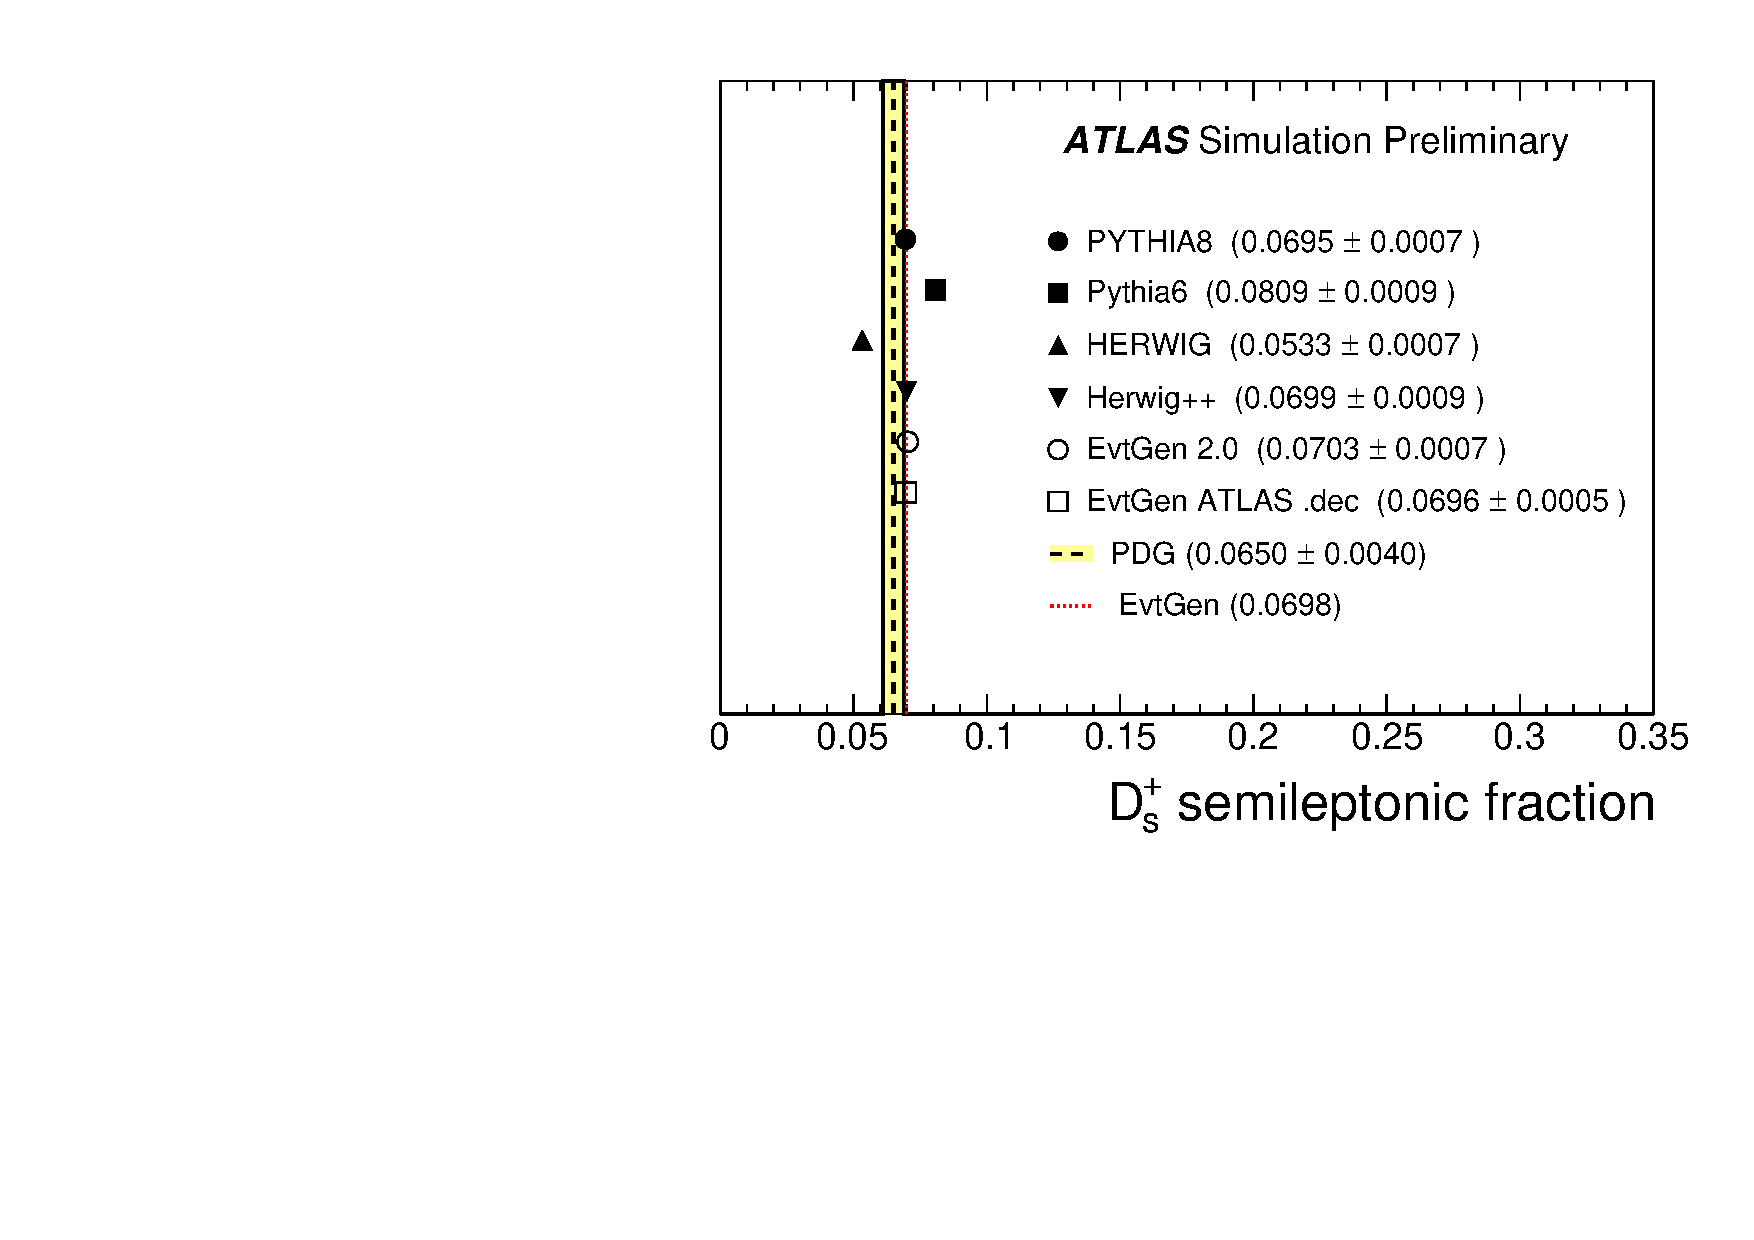
\includegraphics[width=\textwidth]{evtgen/figures/EvtGen/h_Ds_sl.pdf}
\end{subfigure}
\begin{subfigure}[]{0.45\textwidth}
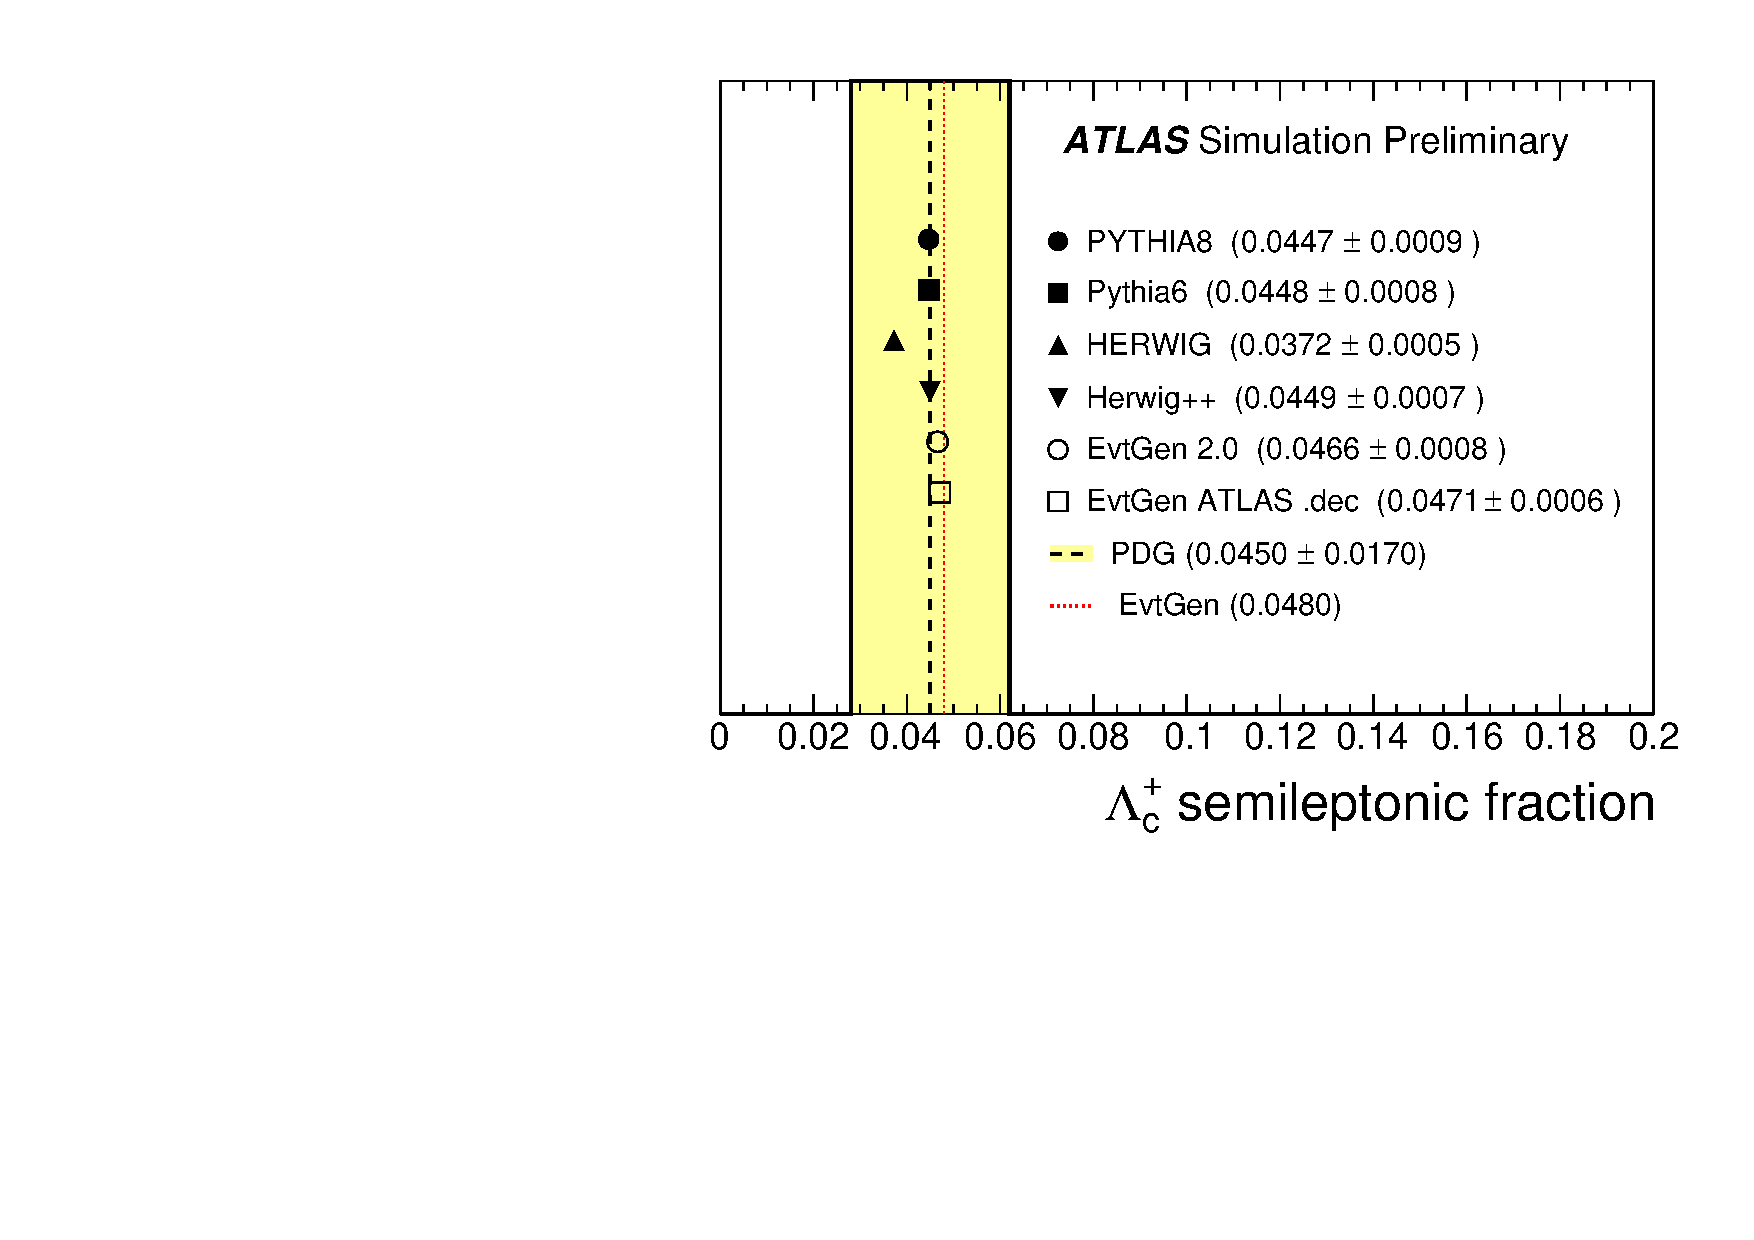
\includegraphics[width=\textwidth]{evtgen/figures/EvtGen/h_Lambdac_sl.pdf}
\end{subfigure}
\caption{Comparison of semileptonic branching fraction $D\rightarrow e^-\overline{\nu_e} X$
of the weakly decaying charm hadrons 
(a) \Dzero, (b) \Dplus, (c) \Ds\ and (d) \Lc~
in four different generators,
\Pythia\ version 427.2, \PythiaE\ version 175, \Herwigpp\  version 2.6.3 and \Herwig\ version 6.520.2, 
both with and without
\EvtGen.  
\EvtGen\ version 2.0 is used with the particle properties table provided with \EvtGen\ and with 
its standard inclusive decay table DECAY\_2010.DEC, as well as a custom decay table with developed for ATLAS with the most up to date semileptonic fractions from the PDG.
Only decays where the electron is the direct decay product of the charm are included.
The values of the $D^0$, $D^+$, $D^+_s$ and $\Lambda^+_c$~semileptonic fractions in this default 
\EvtGen\  particle properties table differ from the world averages listed by the PDG~\cite{PhysRevD.86.010001}.}
\label{fig:csl}
\end{figure}
\begin{figure}
\centering
\begin{subfigure}[]{0.45\textwidth}
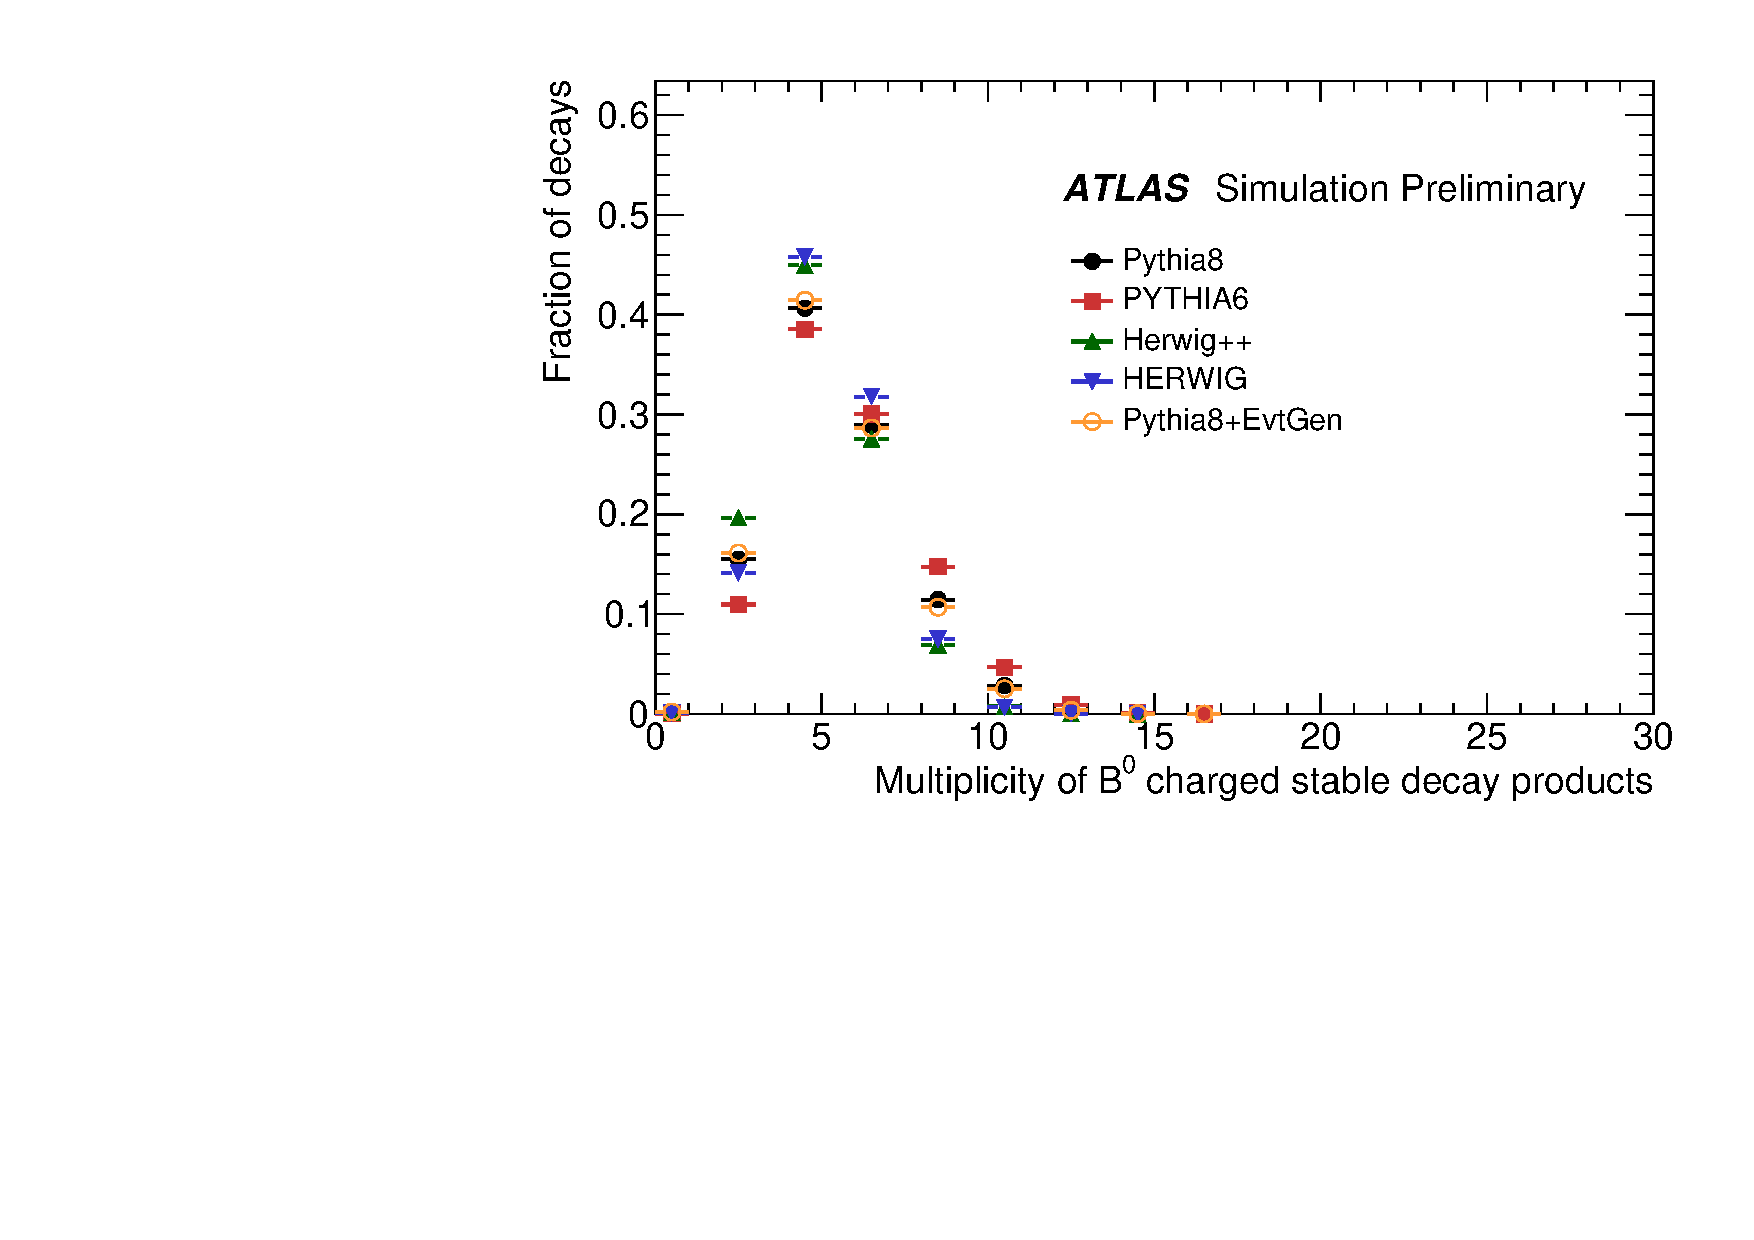
\includegraphics[width=\textwidth]{evtgen/figures/EvtGen/B0/h_species_ncharge.pdf}
\end{subfigure}
\begin{subfigure}[]{0.45\textwidth}
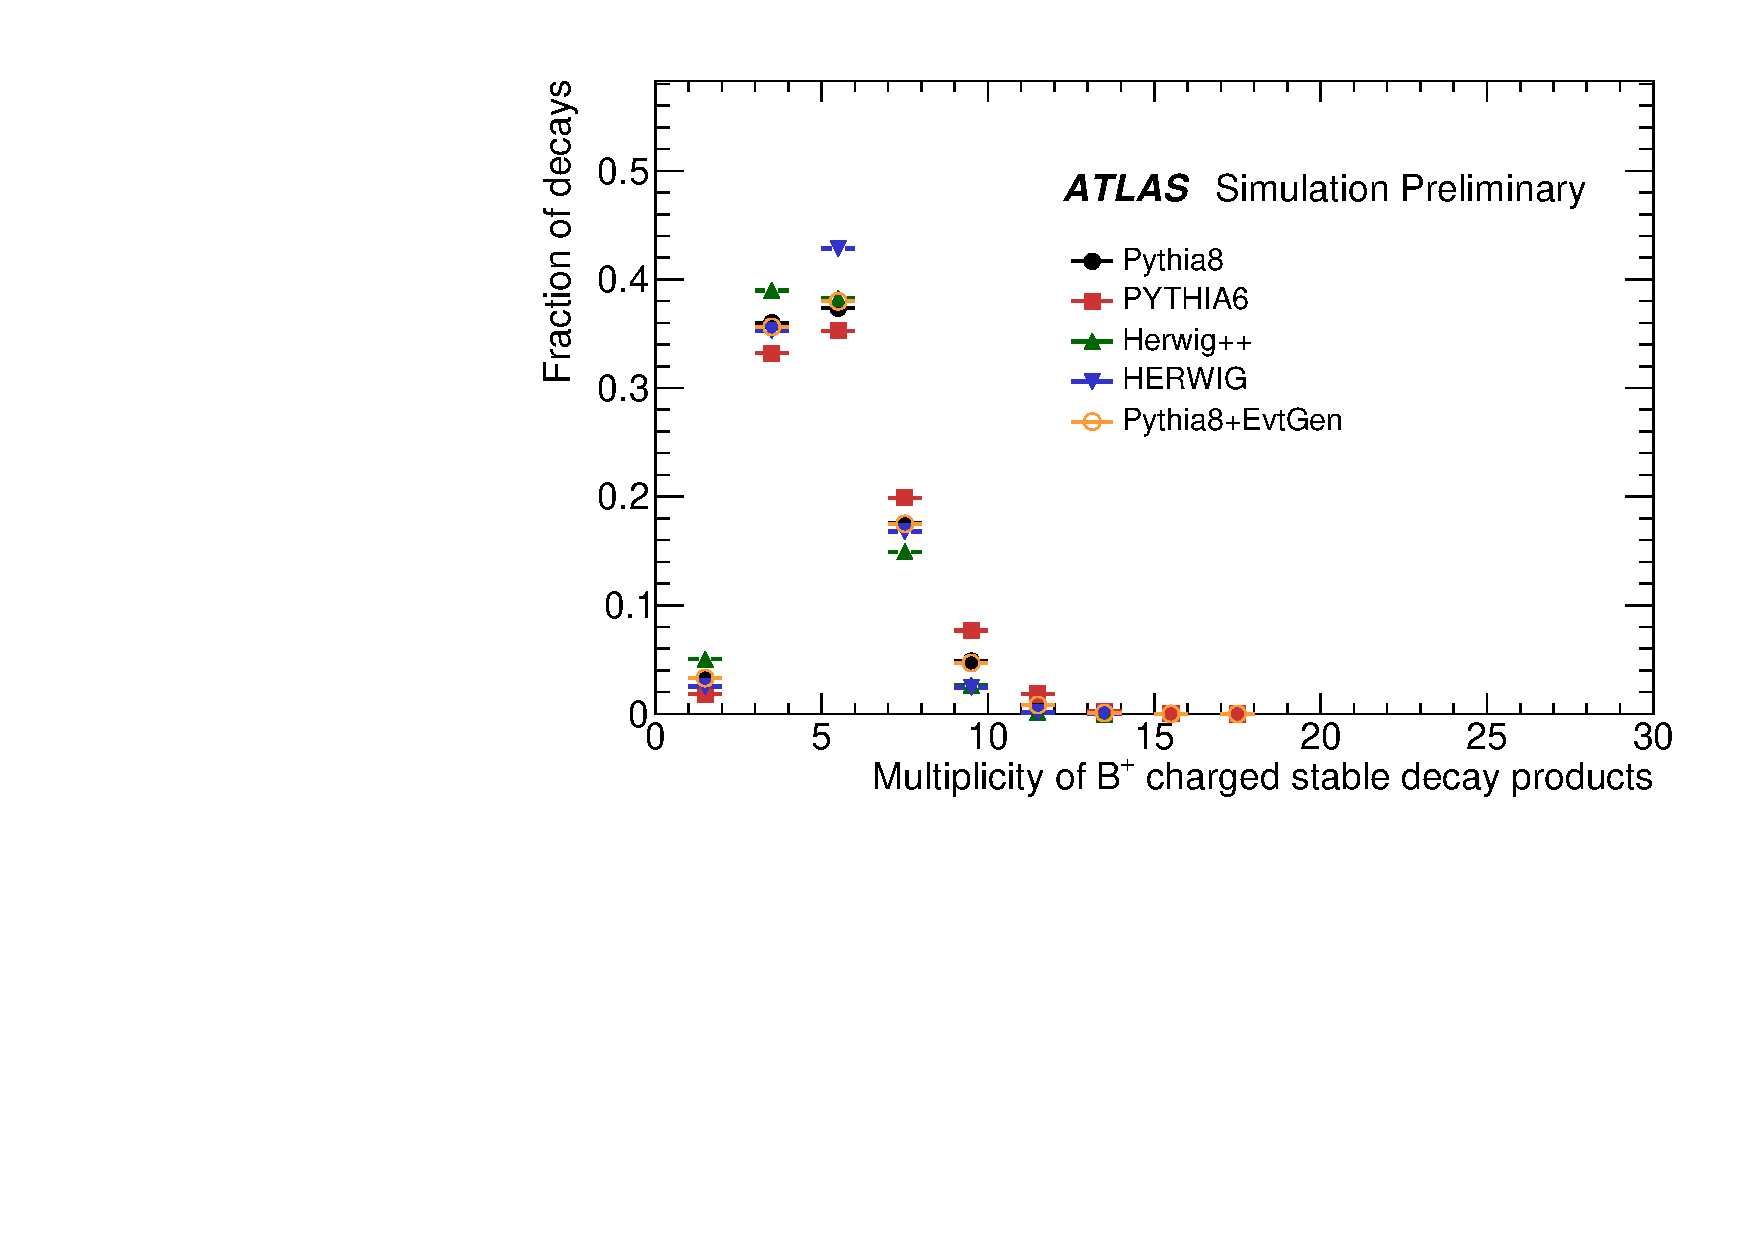
\includegraphics[width=\textwidth]{evtgen/figures/EvtGen/B+/h_species_ncharge.pdf}
\end{subfigure}\\
\begin{subfigure}[]{0.45\textwidth}
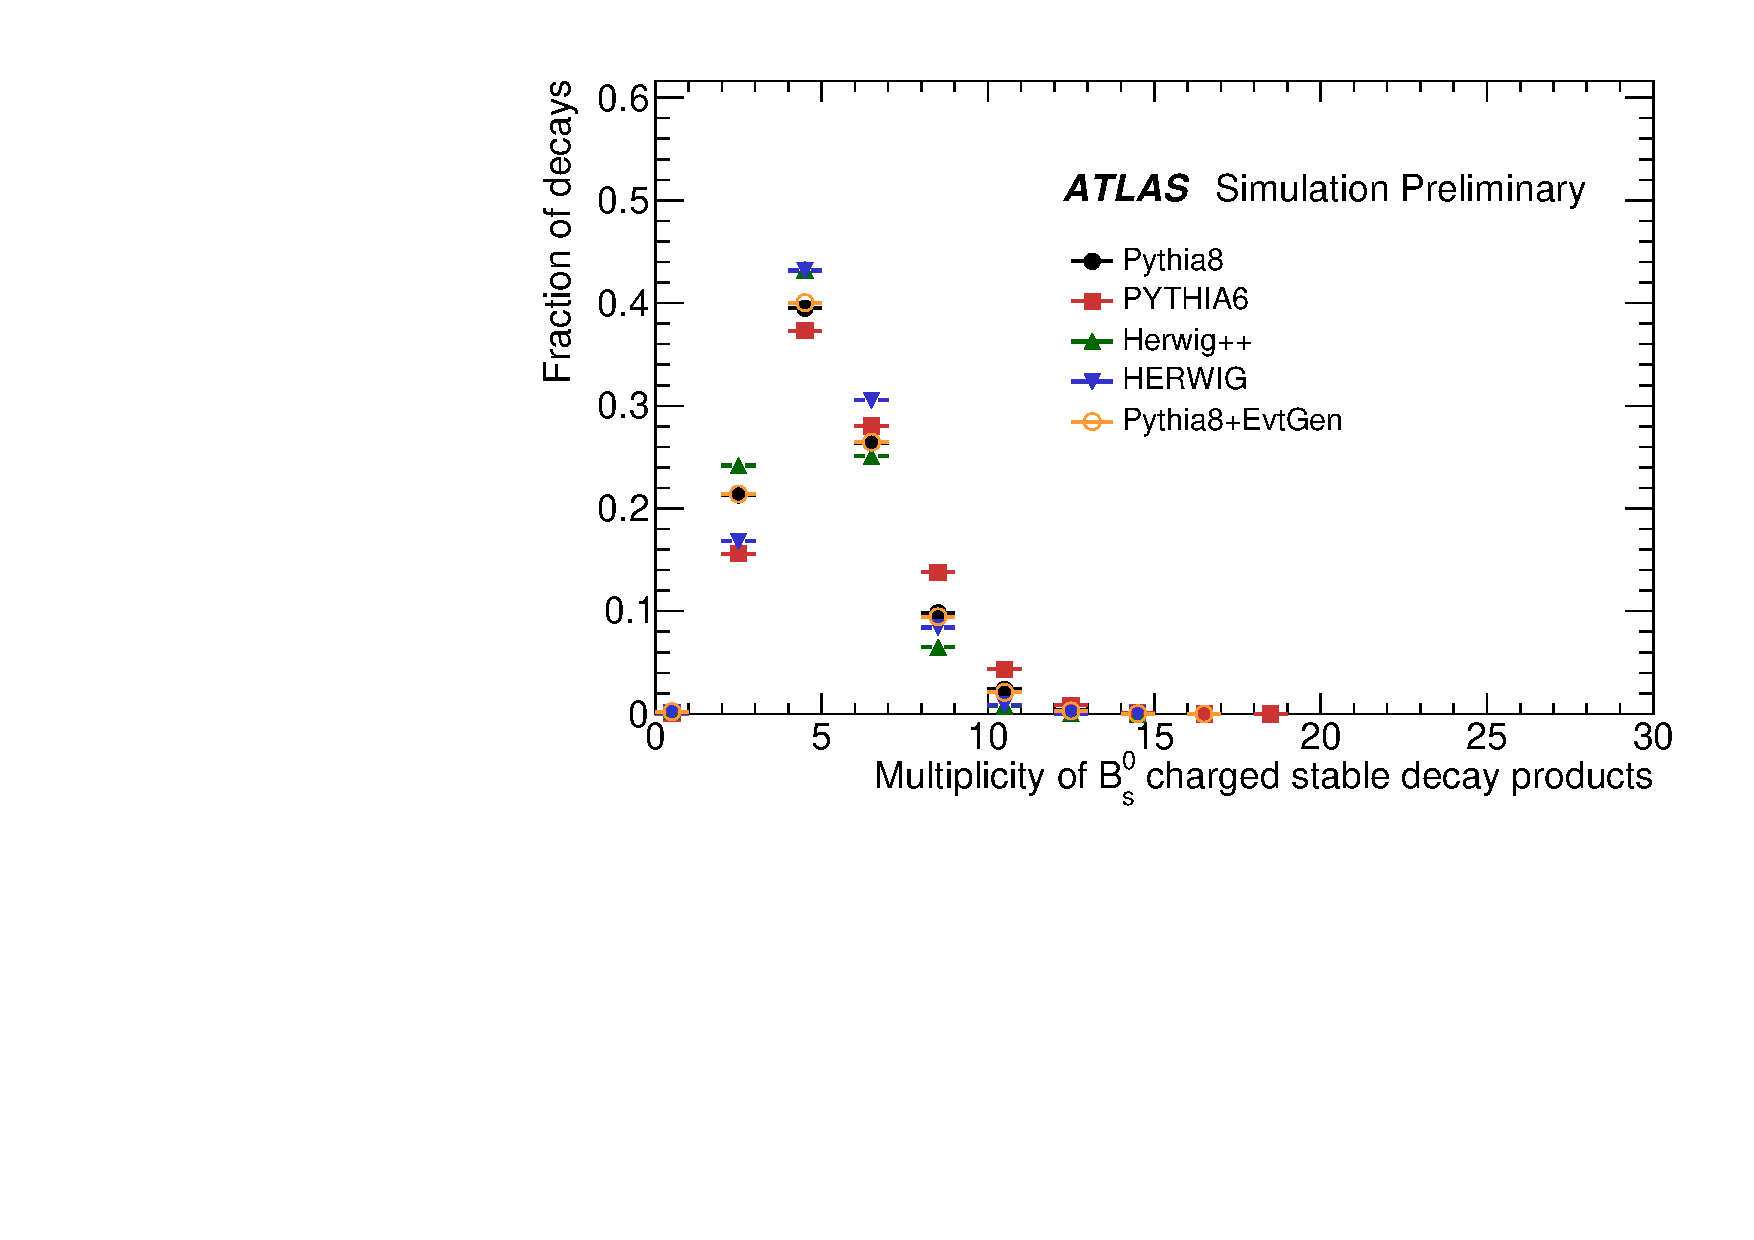
\includegraphics[width=\textwidth]{evtgen/figures/EvtGen/Bs0/h_species_ncharge.pdf}
\end{subfigure}
\begin{subfigure}[]{0.45\textwidth}
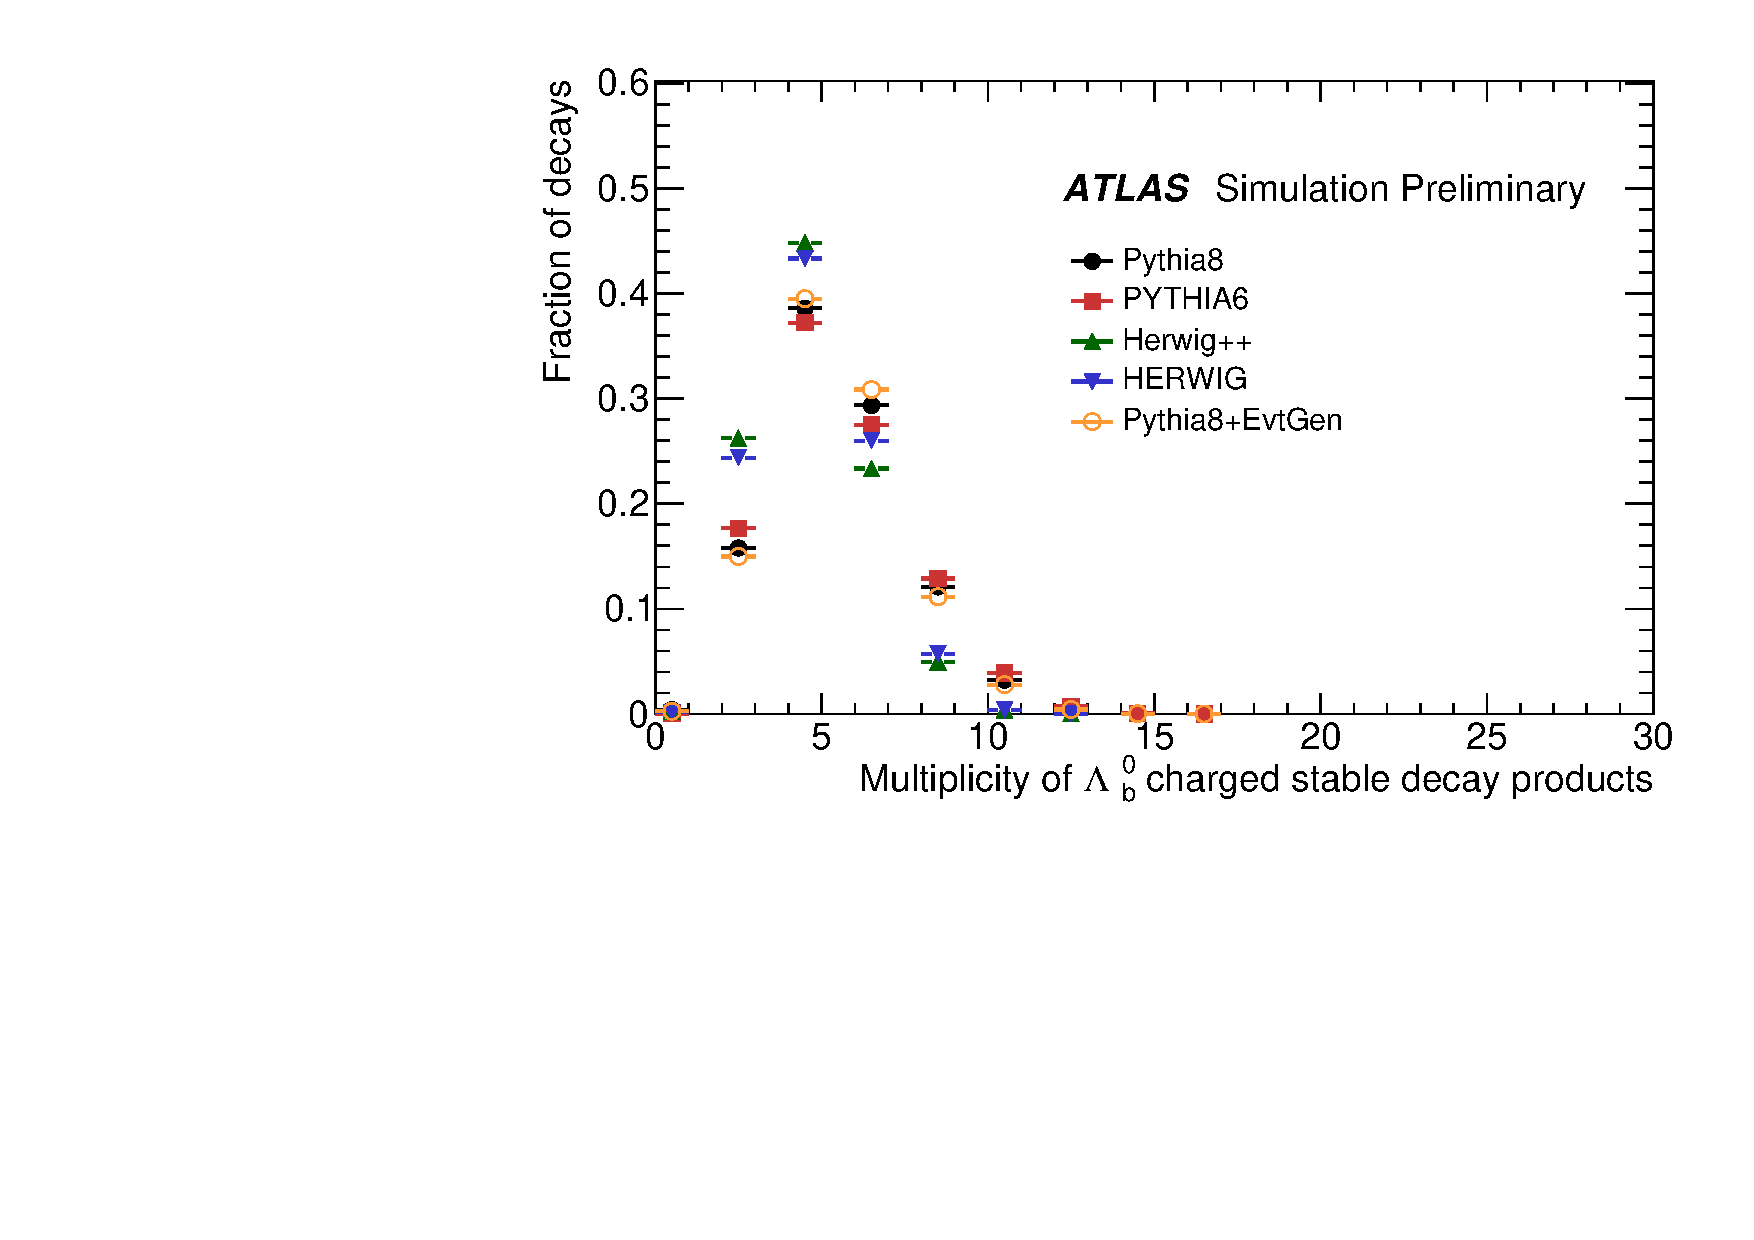
\includegraphics[width=\textwidth]{evtgen/figures/EvtGen/Lambdab0/h_species_ncharge.pdf}
\end{subfigure}
\caption{Comparison of the multiplicity of charged, stable decay products for the weakly decaying bottom hadrons 
(a) $B_0$, (b) $B^{+}$, (c) \Bs~ and (d) \Lb~
in \PythiaE,~ \Pythia,~ \Herwigpp,~\Herwig\ and \EvtGen. A stable particle is defined
as a particle with a proper lifetime $c\tau_{0}>10$~mm. }
\label{fig:bcharge}
\end{figure}

\begin{figure}
\centering
\begin{subfigure}[]{0.45\textwidth}
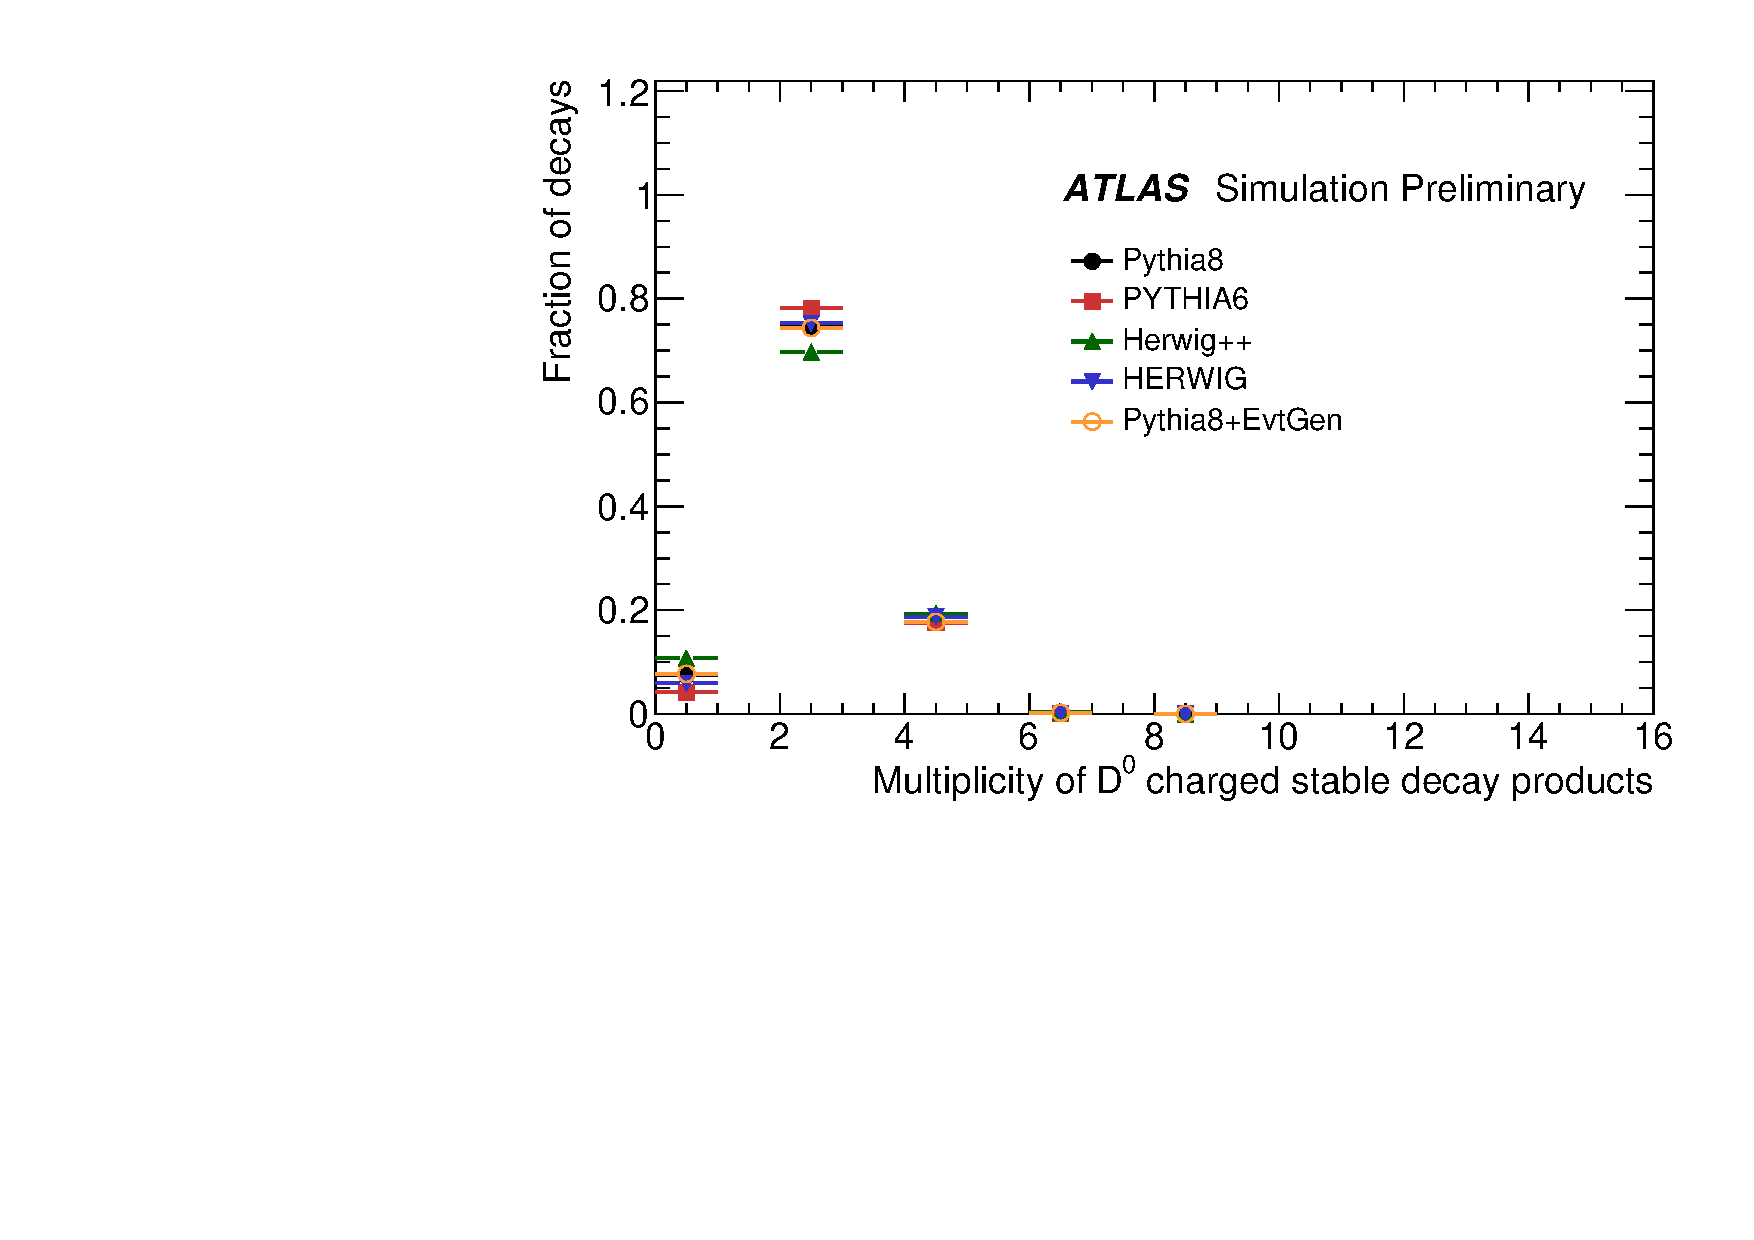
\includegraphics[width=\textwidth]{evtgen/figures/EvtGen/D0/h_species_ncharge.pdf}
\end{subfigure}
\begin{subfigure}[]{0.45\textwidth}
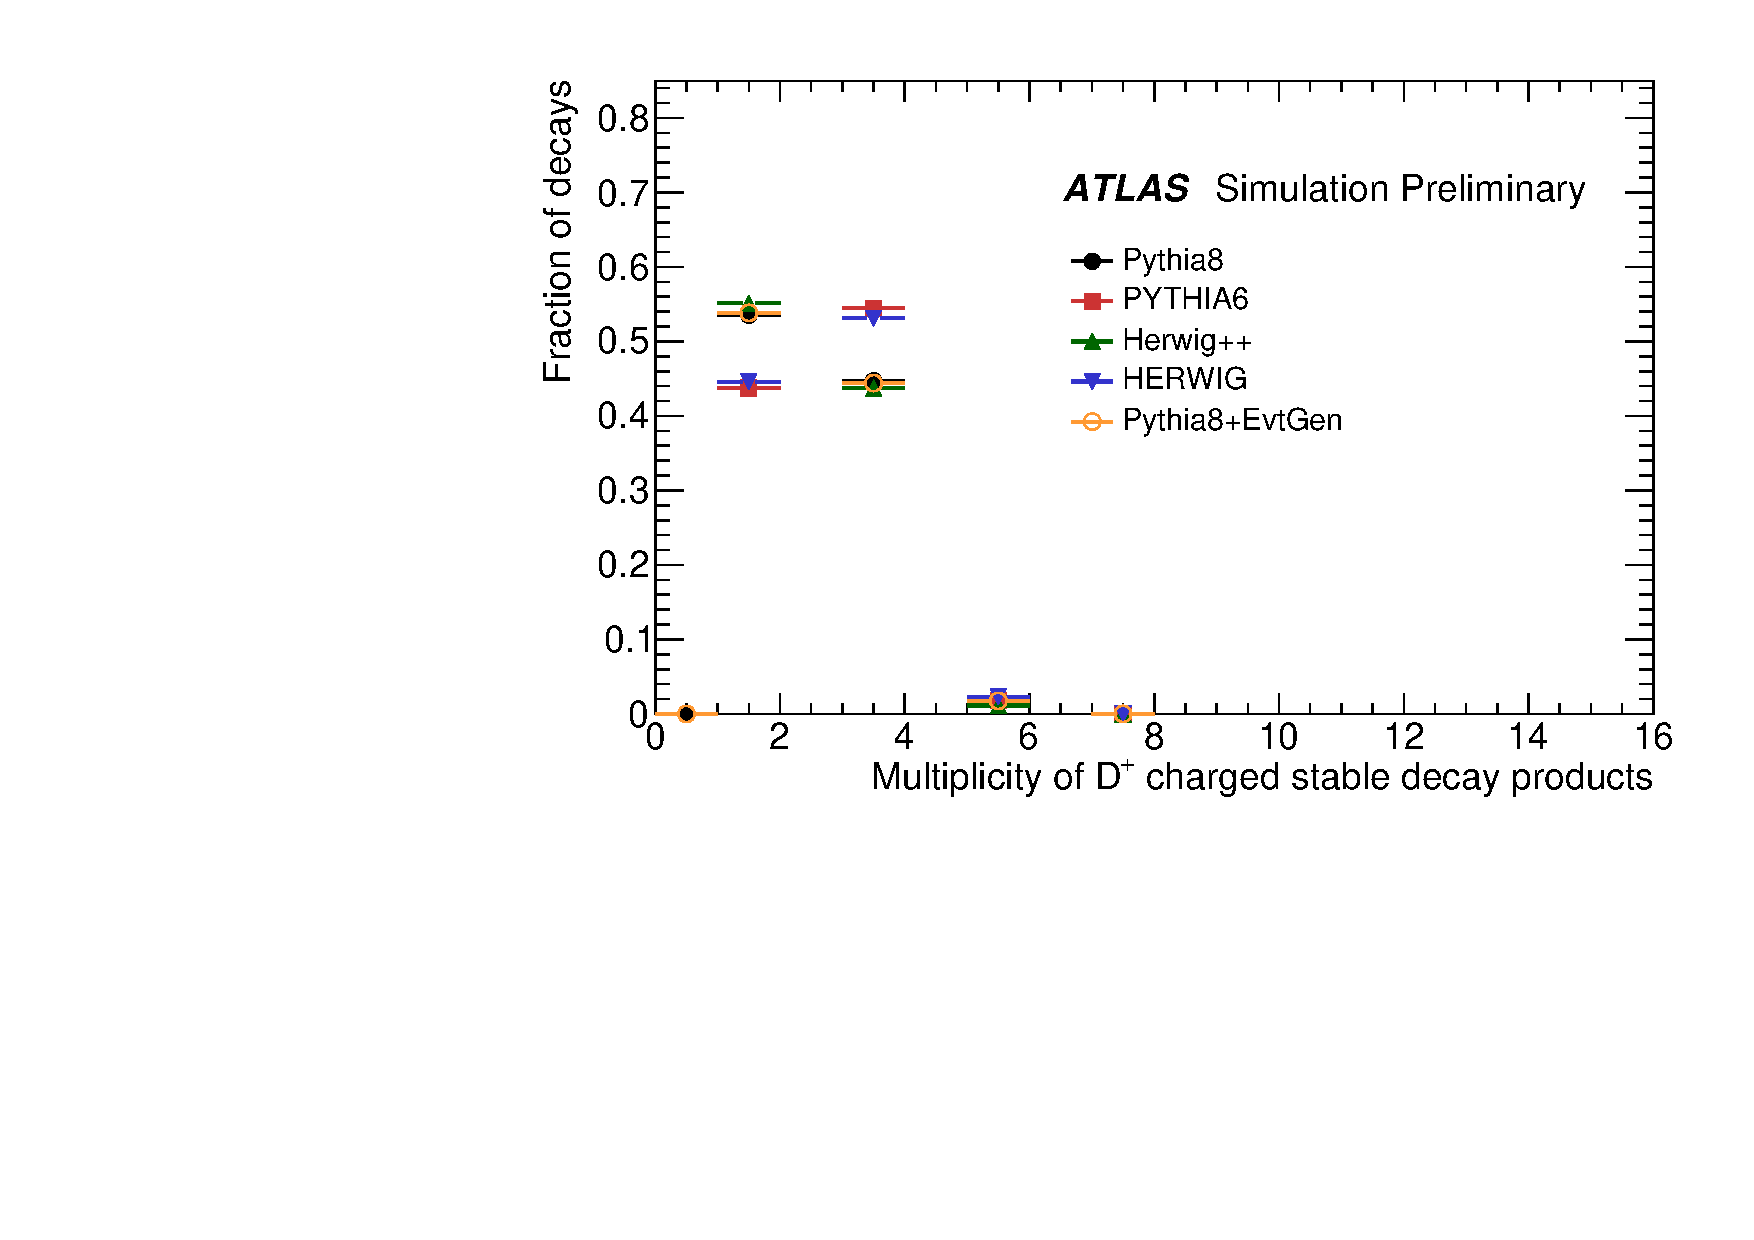
\includegraphics[width=\textwidth]{evtgen/figures/EvtGen/D+/h_species_ncharge.pdf}
\end{subfigure}\\
\begin{subfigure}[]{0.45\textwidth}
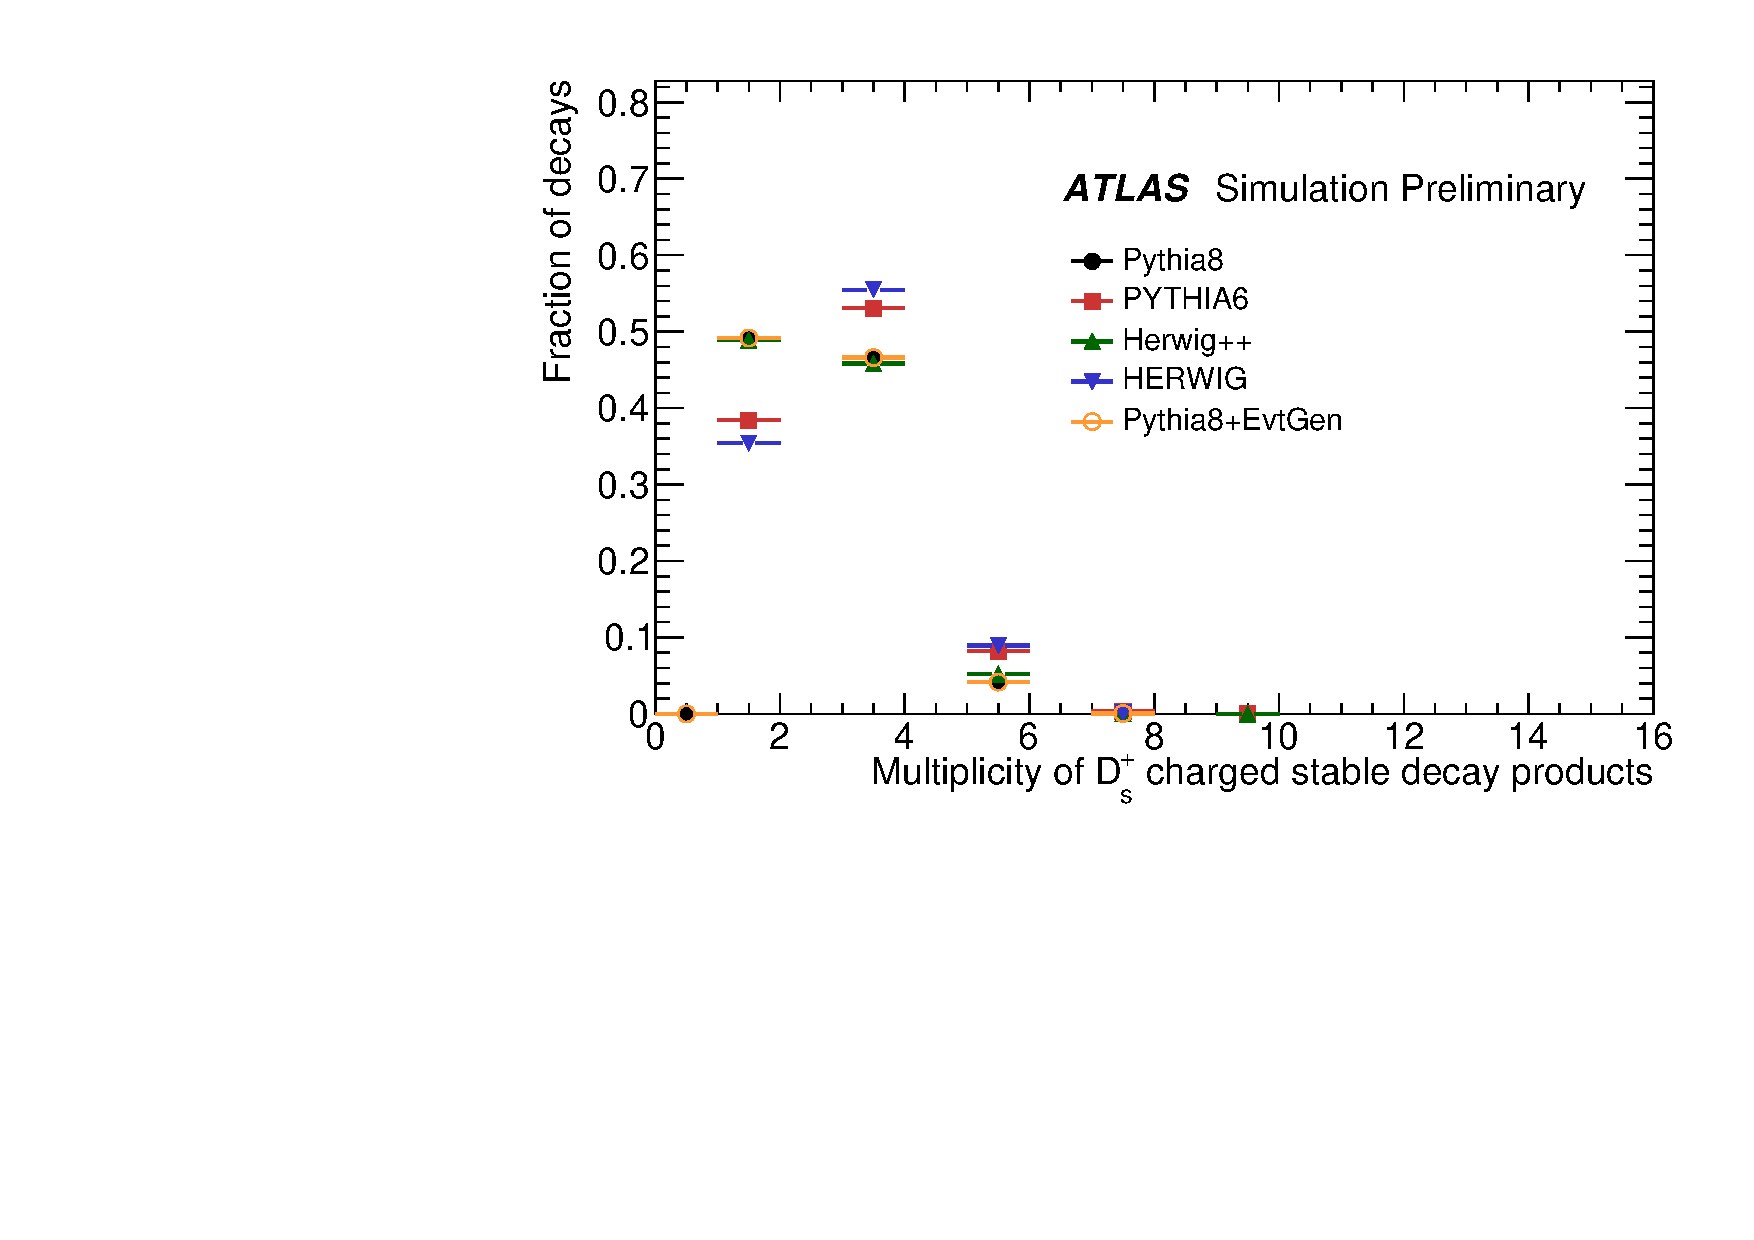
\includegraphics[width=\textwidth]{evtgen/figures/EvtGen/Ds+/h_species_ncharge.pdf}
\end{subfigure}
\begin{subfigure}[]{0.45\textwidth}
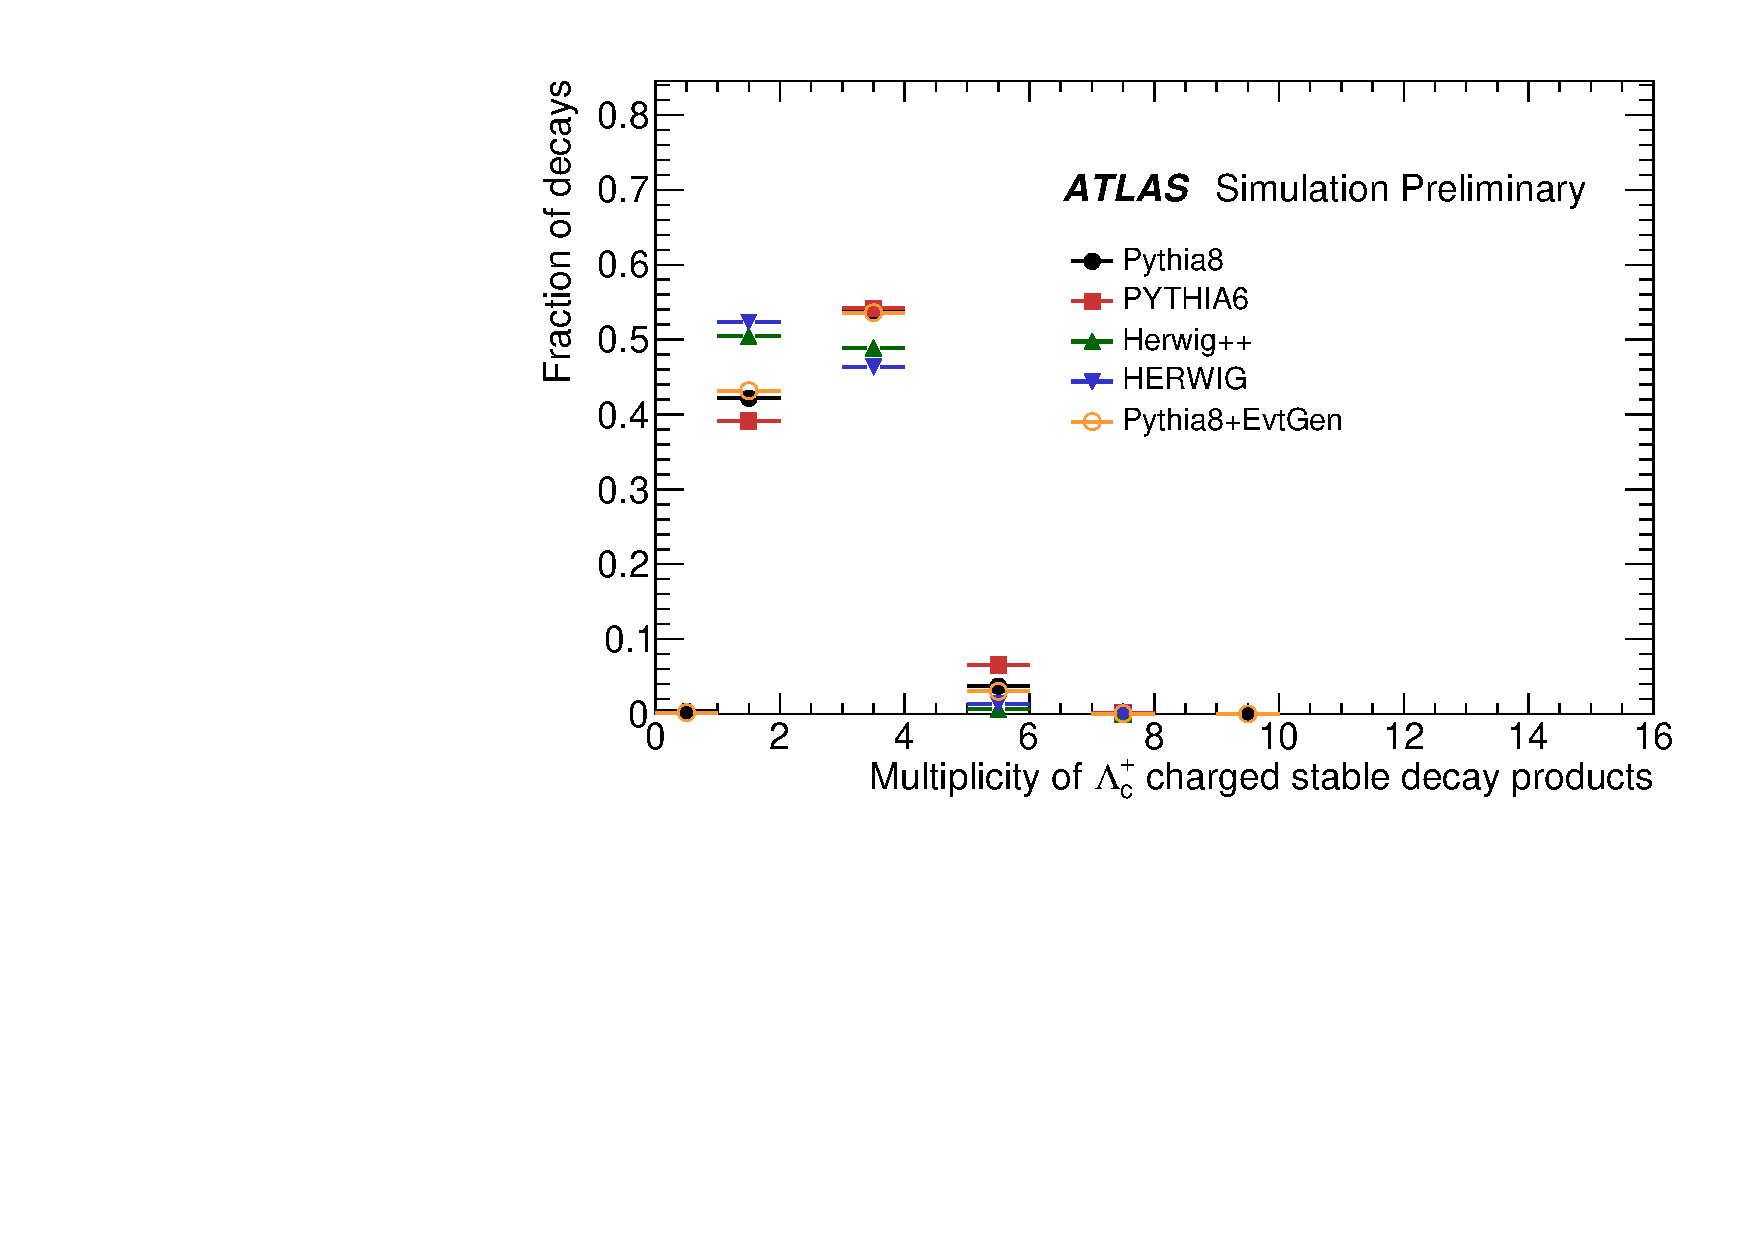
\includegraphics[width=\textwidth]{evtgen/figures/EvtGen/Lambdac+/h_species_ncharge.pdf}
\end{subfigure}
\caption{Comparison of multiplicity of charged, stable decay products for the weakly decaying 
charm hadrons 
(a) \Dzero,~ (b) \Dplus,~ (c) \Ds\ and (d) \Lc~
in \PythiaE,~ \Pythia,~ \Herwigpp,~\Herwig\ and \EvtGen.  A stable particle is defined
as a particle with a proper lifetime $c\tau_{0}>10$~mm. } 
\label{fig:ccharge}
\end{figure}

\begin{figure}
\centering
\begin{subfigure}[]{0.45\textwidth}
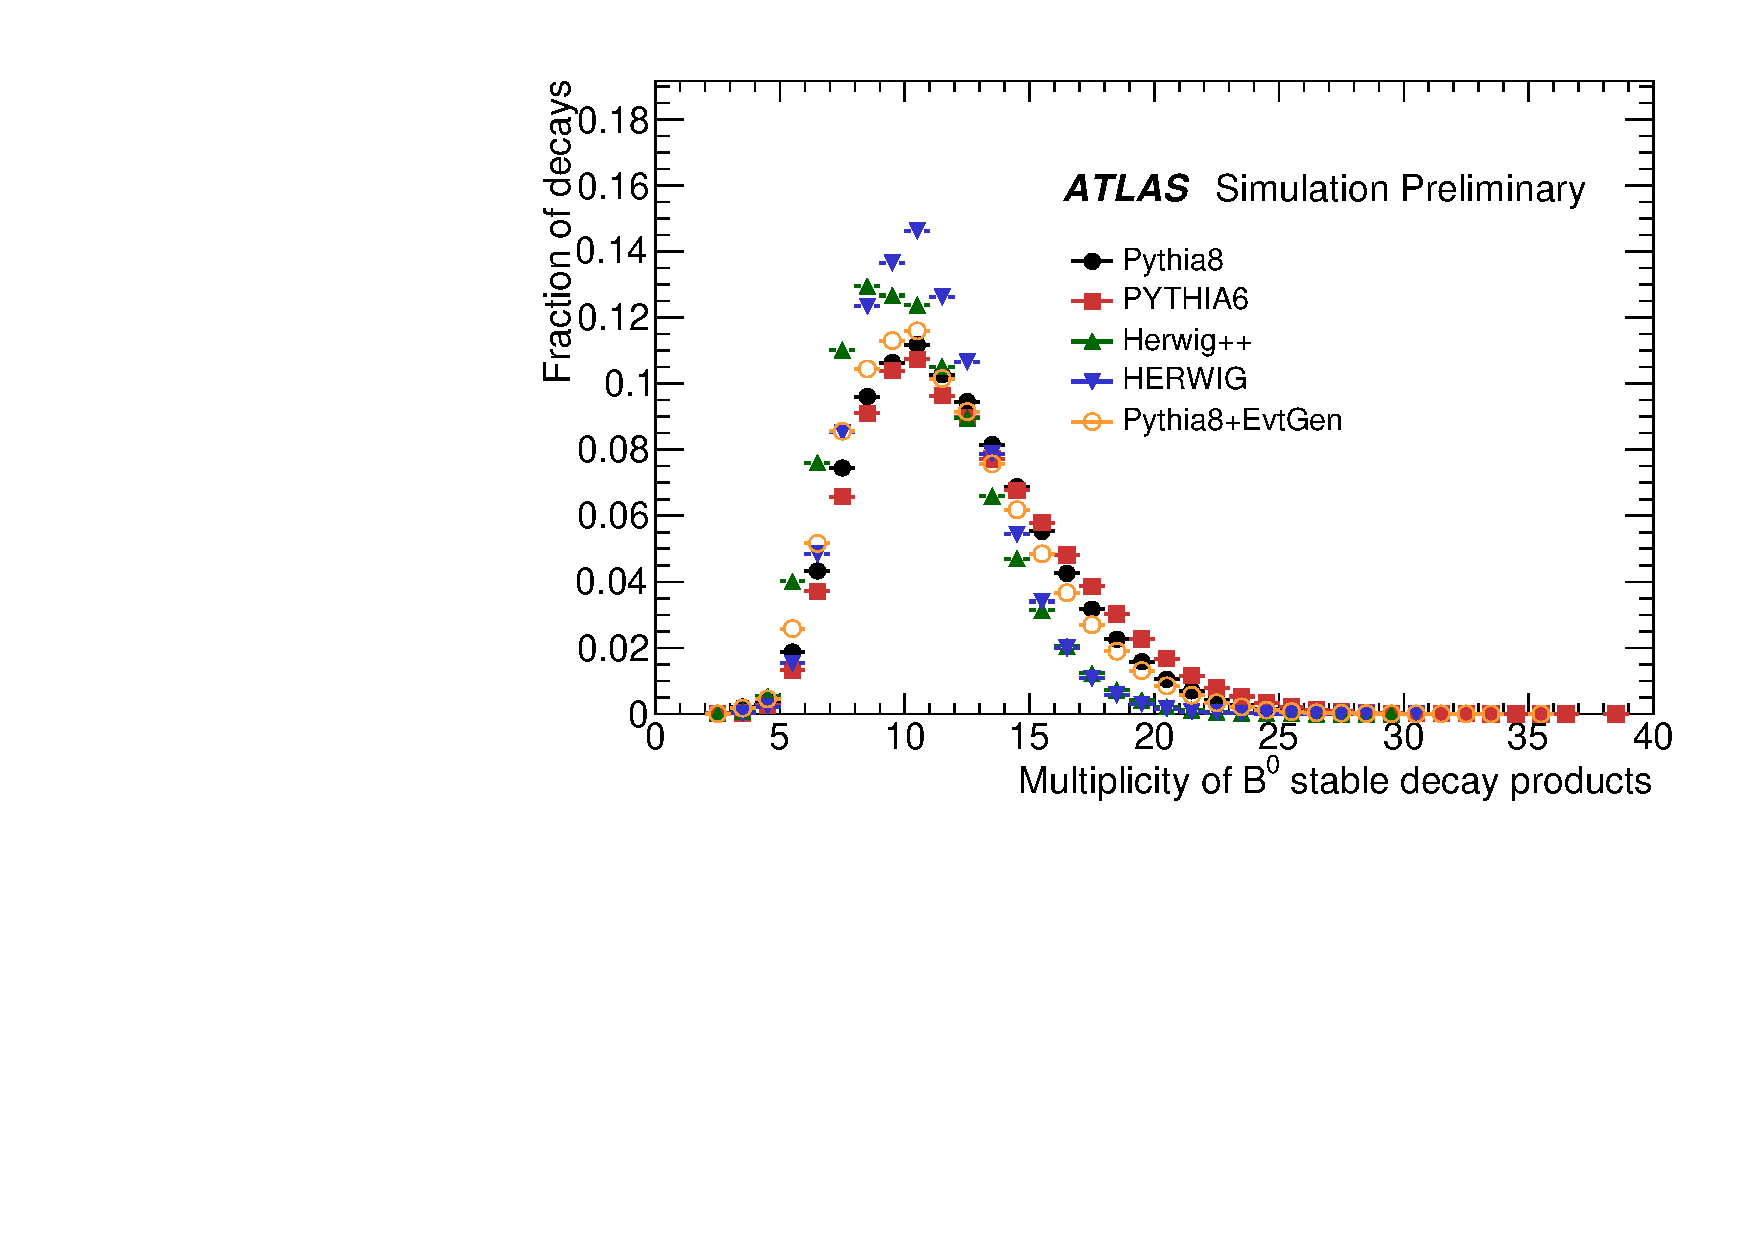
\includegraphics[width=\textwidth]{evtgen/figures/EvtGen/B0/h_species_multiplicity.pdf}
\end{subfigure}
\begin{subfigure}[]{0.45\textwidth}
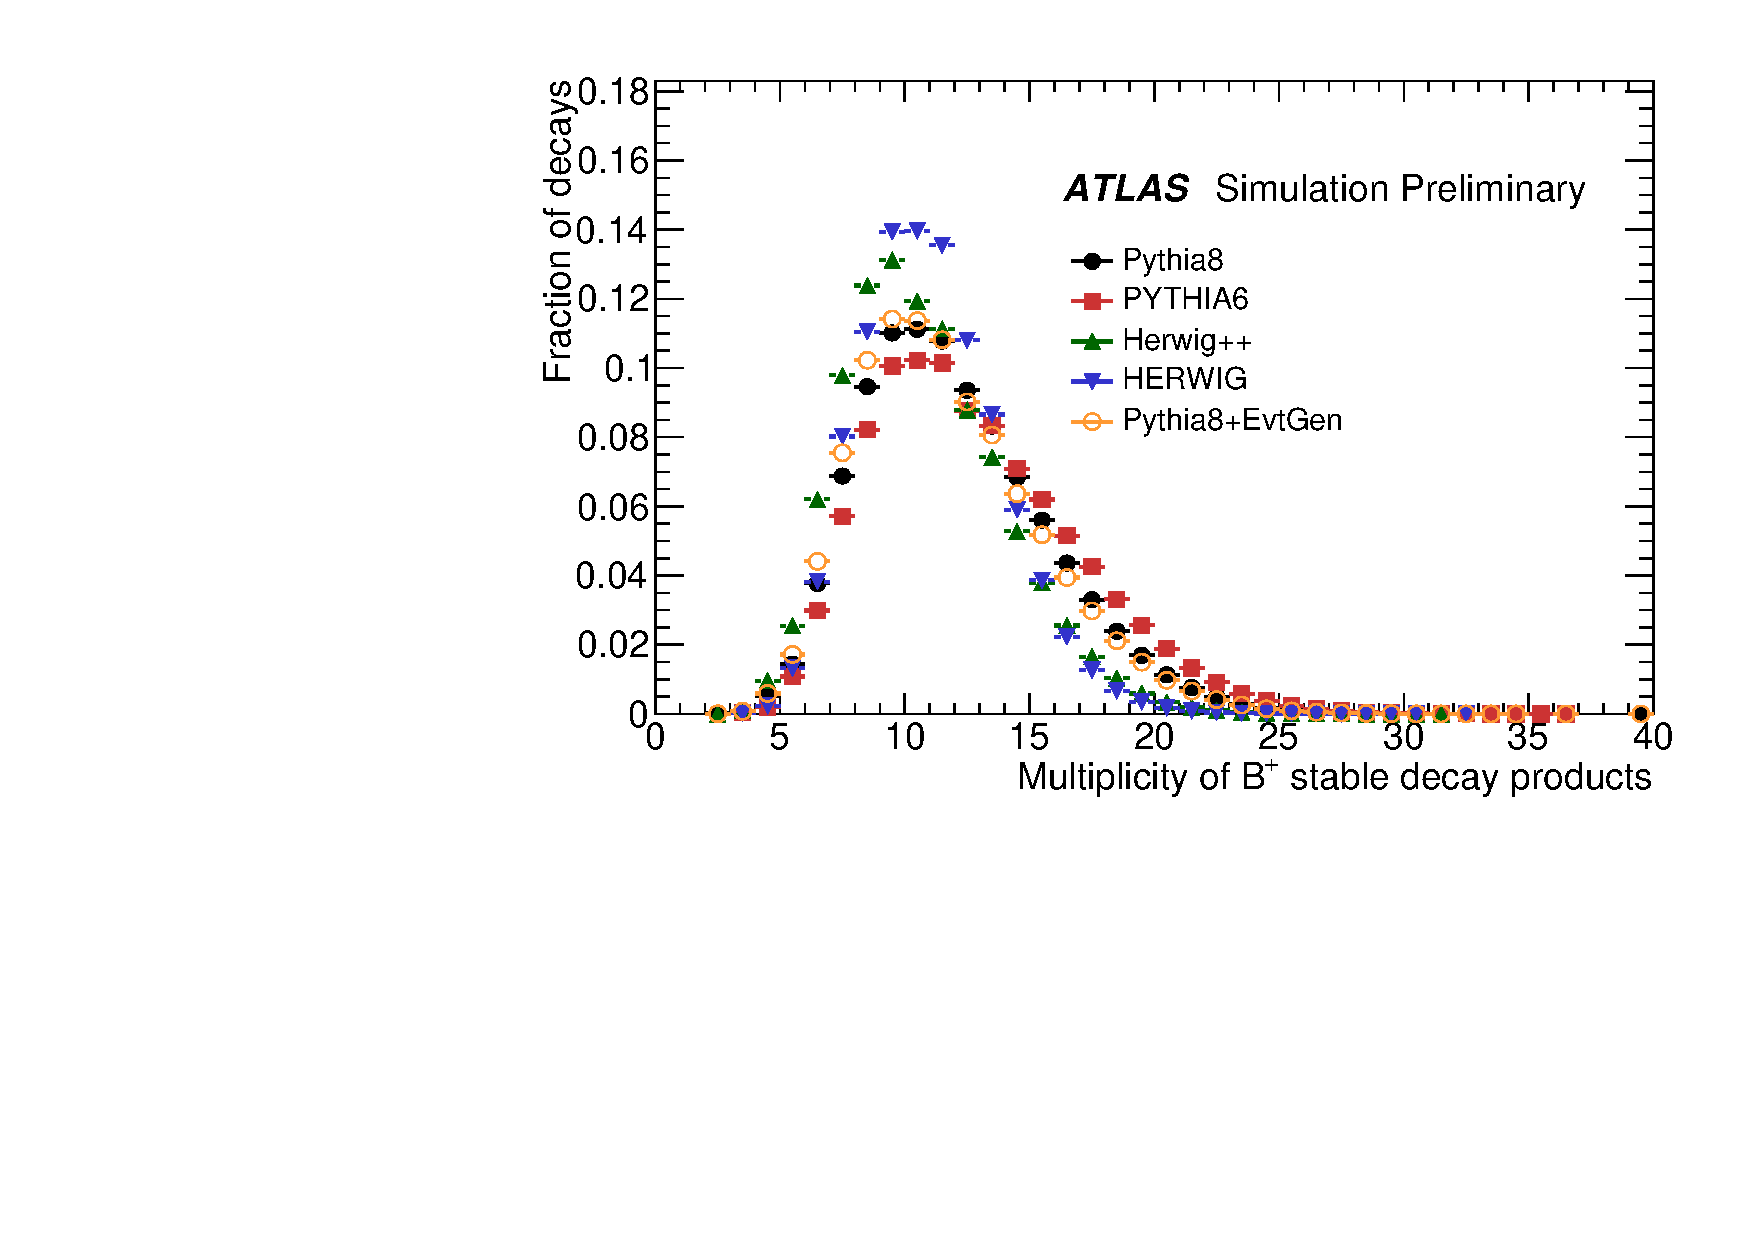
\includegraphics[width=\textwidth]{evtgen/figures/EvtGen/B+/h_species_multiplicity.pdf}
\end{subfigure}\\
\begin{subfigure}[]{0.45\textwidth}
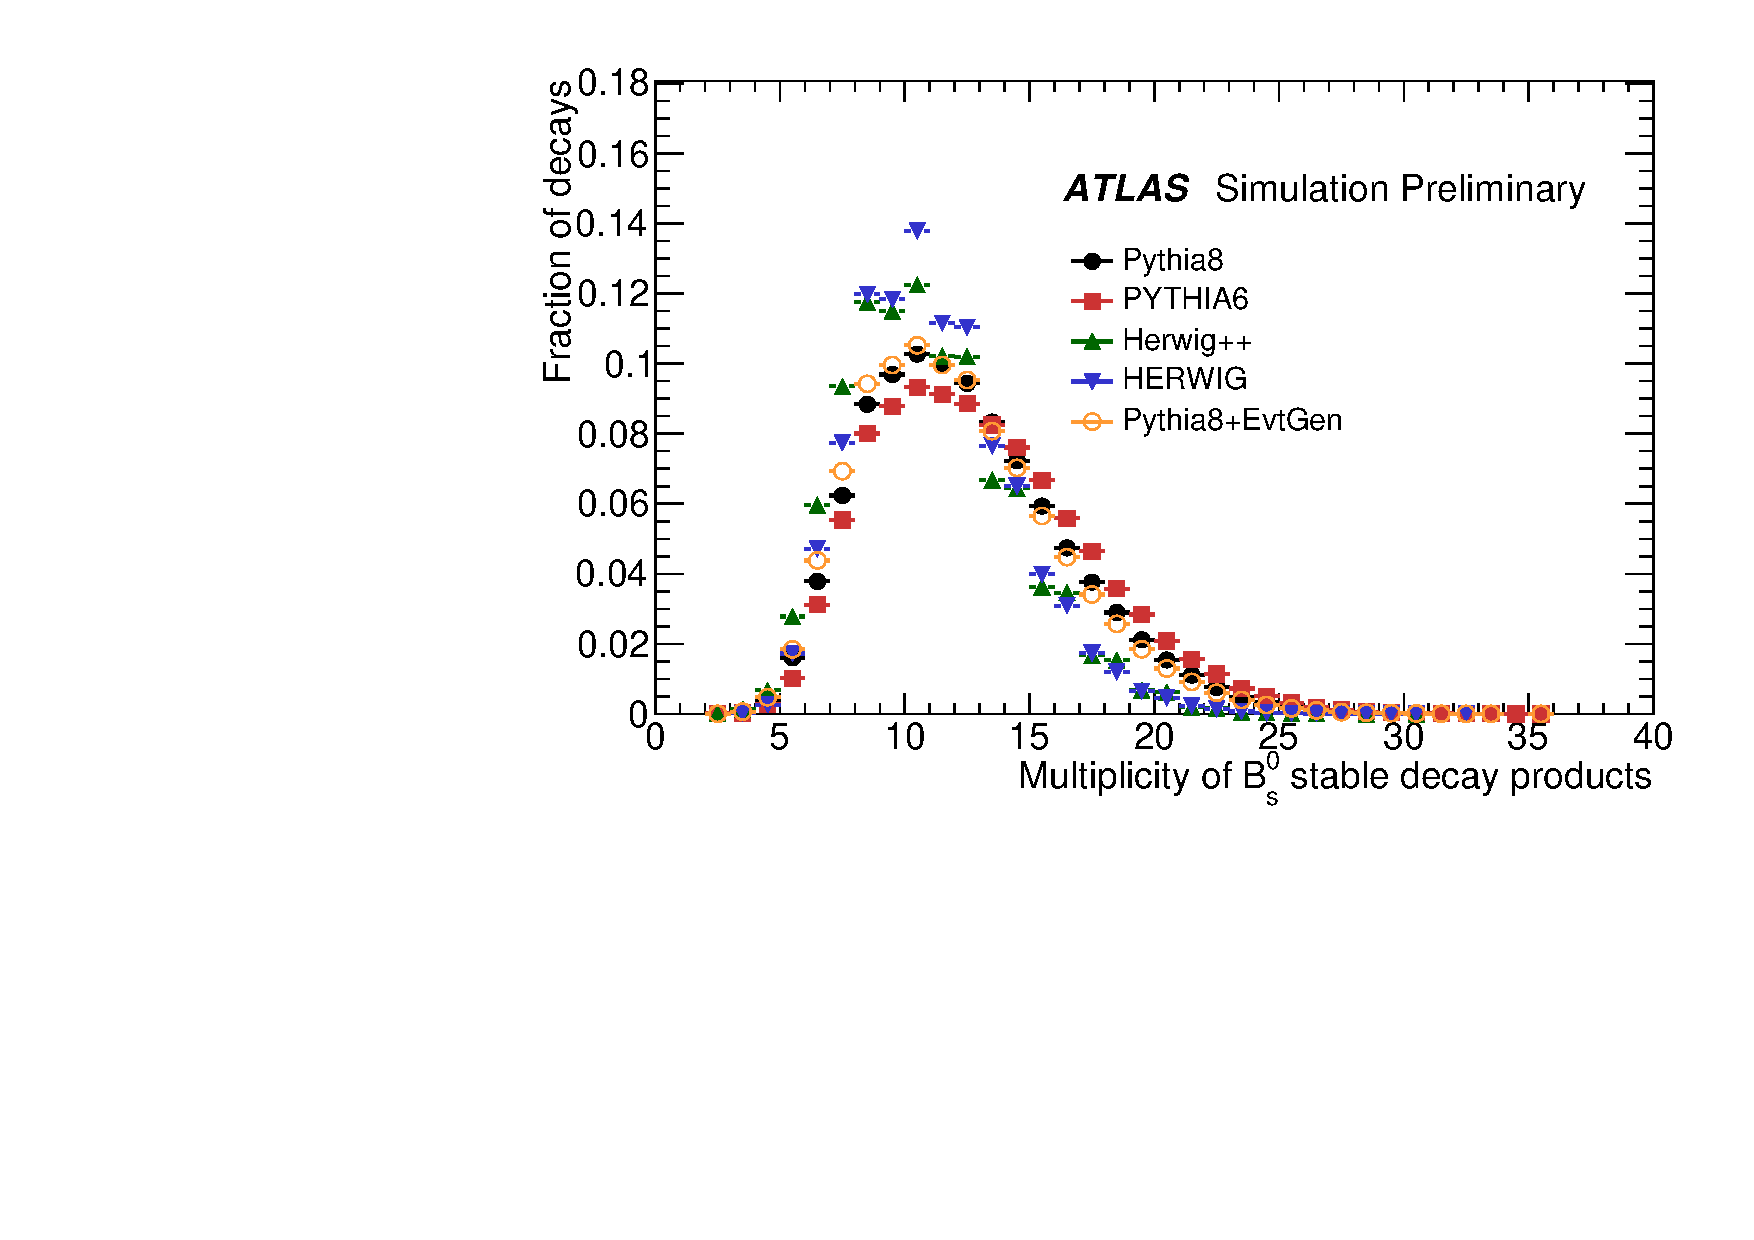
\includegraphics[width=\textwidth]{evtgen/figures/EvtGen/Bs0/h_species_multiplicity.pdf}
\end{subfigure}
\begin{subfigure}[]{0.45\textwidth}
\includegraphics[width=\textwidth]{evtgen/figures/EvtGen/Lambdab0/h_species_multiplicity.pdf}
\end{subfigure}
\caption{Comparison of the multiplicity of stable decay products for the weakly decaying bottom hadrons 
(a) \Bo,~ (b) \Bp,~ (c) \Bs~ and (d) \Lb~
in \PythiaE,~ \Pythia,~ \Herwigpp,~\Herwig\ and \EvtGen.  A stable particle is defined
as a particle with a proper lifetime $c\tau_{0}>10$~mm. }
\label{fig:bmult}
\end{figure}

\begin{figure}
\centering
\begin{subfigure}[]{0.45\textwidth}
\includegraphics[width=\textwidth]{evtgen/figures/EvtGen/D0/h_species_multiplicity.pdf}
\end{subfigure}
\begin{subfigure}[]{0.45\textwidth}
\includegraphics[width=\textwidth]{evtgen/figures/EvtGen/D+/h_species_multiplicity.pdf}
\end{subfigure}\\
\begin{subfigure}[]{0.45\textwidth}
\includegraphics[width=\textwidth]{evtgen/figures/EvtGen/Ds+/h_species_multiplicity.pdf}
\end{subfigure}
\begin{subfigure}[]{0.45\textwidth}
\includegraphics[width=\textwidth]{evtgen/figures/EvtGen/Lambdac+/h_species_multiplicity.pdf}
\end{subfigure}
\caption{Comparison of the multiplicity of stable decay products for the weakly decaying 
charm hadrons 
(a) \Dzero,~ (b) \Dplus,~ (c) \Ds\ and (d) \Lc~ in \PythiaE,~ \Pythia,~ \Herwigpp,~\Herwig\ and \EvtGen.
A stable particle is defined
as a particle with a proper lifetime $c\tau_{0}>10$~mm. }
\label{fig:cmult}
\end{figure}




\begin{table}
\begin{center}
\begin{tabular}{|c|c|c|c|c|c|}
\hline
\multicolumn{6}{|c|}{Multiplicity of charged, stable decay products} \\
\hline \hline
Particle & \PythiaE & \Pythia & \Herwigpp & \Herwig & \PythiaE +\EvtGen \\ \hline
\Bo & $ 4.928 \pm 0.006 $ & $ 5.336 \pm 0.006 $ & $ 4.475 \pm 0.005 $ & $ 4.690 \pm 0.005 $ & $ 4.853 \pm 0.004 $ \\
\Bp & $ 4.754 \pm 0.005 $ & $ 5.102 \pm 0.006 $ & $ 4.435 \pm 0.005 $ & $ 4.636 \pm 0.005 $ & $ 4.750 \pm 0.004 $\\
\Bs & $ 4.661 \pm 0.012 $ & $ 5.136 \pm 0.013 $ & $ 4.319 \pm 0.010 $ & $ 4.665 \pm 0.011 $ & $ 4.623 \pm 0.008 $ \\
$\Lambda_b^{0}$ & $ 4.976 \pm 0.018 $ & $ 5.010 \pm 0.015 $ & $ 4.153 \pm 0.011 $ & $ 4.280 \pm 0.012 $ & $ 4.957 \pm 0.013 $ \\
\Dzero & $ 2.215 \pm 0.003 $ & $ 2.273 \pm 0.003 $ & $ 2.182 \pm 0.003 $ & $ 2.263 \pm 0.003 $ & $ 2.208 \pm 0.002 $  \\
\Dplus & $ 1.965 \pm 0.003 $ & $ 2.161 \pm 0.004 $ & $ 1.920 \pm 0.004 $ & $ 2.154 \pm 0.005 $ & $ 1.958 \pm 0.002 $ \\
\Ds & $ 2.103 \pm 0.007 $ & $ 2.410 \pm 0.008 $ & $ 2.129 \pm 0.008 $ & $ 2.476 \pm 0.009 $ & $ 2.102 \pm 0.005 $ \\
$\Lambda_c^{+}$ & $ 2.222 \pm 0.010 $ & $ 2.353 \pm 0.009 $ & $ 2.004 \pm 0.008 $ & $ 1.980 \pm 0.006 $ & $ 2.193 \pm 0.007 $ \\ \hline
\end{tabular}
\caption{Mean number of charged, stable decay products for the weakly decaying 
bottom and charm hadrons species
in \PythiaE,~ \Pythia,~ \Herwigpp,~\Herwig\ and \EvtGen.  A stable particle is defined
as a particle with a proper lifetime $c\tau_{0}>10$~mm.}
\label{t:charge}
\end{center}
\end{table}


\begin{table}
\begin{center}
\begin{tabular}{|c|c|c|c|c|c|}
\hline
\multicolumn{6}{|c|}{Multiplicity of stable decay products} \\
\hline \hline
Particle & \PythiaE & \Pythia & \Herwigpp & \Herwig & \PythiaE +\EvtGen \\
\hline
\Bo & $ 11.379 \pm 0.012 $ & $ 11.939 \pm 0.013 $ & $ 9.919 \pm 0.011 $ & $ 10.339 \pm 0.012 $ & $ 10.982 \pm 0.009 $  \\
\Bp & $ 11.527 \pm 0.013 $ & $ 12.263 \pm 0.014 $ & $ 10.283 \pm 0.012 $ & $ 10.550 \pm 0.012 $ & $ 11.250 \pm 0.009 $ \\
\Bs & $ 11.933 \pm 0.030 $ & $ 12.552 \pm 0.032 $ & $ 10.516 \pm 0.024 $ & $ 10.706 \pm 0.024 $ & $ 11.631 \pm 0.021 $ \\
$\Lambda_b^{0}$ & $ 11.220 \pm 0.040 $ & $ 11.298 \pm 0.034 $ & $ 9.376 \pm 0.024 $ & $ 10.060 \pm 0.026 $ & $ 10.772 \pm 0.027 $ \\
\Dzero & $ 4.920 \pm 0.006 $ & $ 5.002 \pm 0.006 $ & $ 4.784 \pm 0.006 $ & $ 4.748 \pm 0.007 $ & $ 4.853 \pm 0.004 $ \\
\Dplus & $ 4.344 \pm 0.007 $ & $ 4.554 \pm 0.008 $ & $ 4.053 \pm 0.007 $ & $ 4.437 \pm 0.009 $ & $ 4.265 \pm 0.005 $  \\
\Ds & $ 5.564 \pm 0.017 $ & $ 5.842 \pm 0.019 $ & $ 5.393 \pm 0.019 $ & $ 5.548 \pm 0.019 $ & $ 5.500 \pm 0.012 $ \\
$\Lambda_c^{+}$ & $ 5.007 \pm 0.021 $ & $ 5.100 \pm 0.019 $ & $ 4.219 \pm 0.015 $ & $ 4.485 \pm 0.013 $ & $ 4.751 \pm 0.014 $  \\ 
\hline
\end{tabular}
\caption{Mean number of stable decay products for the weakly decaying 
bottom and charm hadrons species
in \PythiaE,~ \Pythia,~ \Herwigpp,~\Herwig\ and \EvtGen.  A stable particle is defined
as a particle with a proper lifetime $c\tau_{0}>10$~mm.}
\label{t:mult}
\end{center}
\end{table}





%\section{Summary}
%\label{sec:conclusion}
%Studies of heavy flavor production fractions, fragmentation functions and decay properties 
for four MC generators are presented.
Bottom production fractions vary among generators, largely due to large differences
of up to 6.5\%\ in the baryon fraction.  For charm production, 
the generators overestimate the $D^+$ fraction.  The $D^0$ fraction
in \Herwig\ is significantly lower than for the other three generators; \Herwig, \Pythia, and
\PythiaE\ are in good agreement with world average data.
Distributions of $x$ ($x_p$), the fraction of the heavy quark energy (momentum) carried by
the bottom (charm) hadron have been studied using $e^+e^-$ samples generated
with the same showering parameters used in modern LHC tunes.  Differences in the mean value of $x$  
generated differ by up to 5\%\ for bottom and up to 12\%\ for charm.  Studies of $f(z)$,
the fraction of the jet momentum carried by the heavy flavor hadron, from \ttbar\ samples
show good agreement among all the generators except for \Herwigpp, which has a
mean value of $z$ for bottom jets s higher by about 2\%.  Comparisons of $f(z)$ distributions for
high transverse momentum jets indicate that the treatment of heavy flavor pair production
differs between among the generators.
\EvtGen\ was found to improve agreement with PDG values for the decays of heavy flavor particles, but modifications to the standard \EvtGen\ inclusive decay table further improve agreement with the experimental measurements of branching fractions.

%\clearpage
\appendix
\textit{The following appendices are for internal ATLAS circulation only and will be removed before this note is made public.  Appendix C, which lists the changes made to the default EvtGen inclusive decay table,
will be provided as additional information on the ATLAS web page.} 
\section{MC Datasets}
\label{app:datasets}
The EvtGen studies use $t \bar{t}$ samples without EvtGen:
\begin{itemize}
\item mc12\_valid.187003.PowhegHerwigpp\_UE4\_MRSTMCa\_CT10ME\_ttbar\_LF.evgen.EVNT.e2765/
\item mc12\_valid.187002.PowhegPythia\_P2011C\_ttbar\_LeptonFilter.evgen.EVNT.e2765/
\item mc12\_valid.187001.PowhegPythia8\_AU2CT10\_ttbar\_LeptonFilter.evgen.EVNT.e2765/
\item mc12\_valid.187000.PowhegJimmy\_AUET2CT10\_ttbar\_LeptonFilter.evgen.EVNT.e276/
\end{itemize}
The EvtGen studies use $t \bar{t}$ samples with EvtGen 2.0 and custom .dec:
\begin{itemize}
\item mc12\_valid.187007.PowhegHerwigppEvtgen\_UE4\_MRSTMCa\_CT10\_ttbar\_LF.evgen.e2765/
\item mc12\_valid.187006.PowhegPythiaEvtgen\_P2011C\_ttbar\_LeptonFilter.evgen.e2765/
\item mc12\_valid.187005.PowhegPythia8Evtgen\_AU2CT10\_ttbar\_LepFilt.evgen.e2765/
\item mc12\_valid.187004.PowhegJimmyEvtgen\_AUET2CT10\_ttbar\_LepFilt.evgen.e2765/
\end{itemize}

Default decay file for semi-leptonic comparisons:
\begin{itemize}
\item user.jbrosame.Pythia8.Jz4.EvtGen.Nov29.EVGEN\_EXT0/
\end{itemize}

Jz4 samples without EvtGen:
\begin{itemize}
\item FHerwigJz4.py
\item HerwigppJz4.py
\item mc12\_8TeV.129324.Pythia\_AUET2BCTEQ6L1\_jetjet\_JZ4.evgen.EVNT.e1641/
\item mc12\_8TeV.147904.Pythia8\_AU2CT10\_jetjet\_JZ4.evgen.EVNT.e1126/
\end{itemize}

Custom $e+e-$ samples were generated using standard LEP job options, given in ~\ref{app:JO}.


\section{Private samples}
\label{app:JO}
All samples were generated with Athena release 17.2.12.7
\subsection{BELLE: $e+e- \rarrow c \bar{c}$ at $\sqrt{s}=10.6$ GeV}
\subsubsection{\Herwig}
\lstinputlisting[breaklines]{JobOptions/BelleFHerwig.py}
\subsubsection{\Herwigpp}
\lstinputlisting[breaklines]{JobOptions/BelleHerwigpp.py}
\subsubsection{\Pythia}
\lstinputlisting[breaklines]{JobOptions/BellePythia6.py}
\subsubsection{\PythiaE}
\lstinputlisting[breaklines]{JobOptions/BellePythia8.py}
\subsection{LEP: $e+e- \rarrow b \bar{b}$ at $\sqrt{s}=91.2$ GeV}
\subsubsection{\Herwig}
\lstinputlisting[breaklines]{JobOptions/LEPFHerwig.py}
\subsubsection{\Herwigpp}
\lstinputlisting[breaklines]{JobOptions/LEPHerwigpp.py}
\subsubsection{\Pythia}
\lstinputlisting[breaklines]{JobOptions/LEPPythia6.py}
\subsubsection{\PythiaE}
\lstinputlisting[breaklines]{JobOptions/LEPPythia8.py}
\subsection{Jz4: $\sqrt{s}=8$ TeV}
\subsubsection{\Herwig}
\lstinputlisting[breaklines]{JobOptions/FHerwigJz4.py}
\subsubsection{\Herwigpp}
\lstinputlisting[breaklines]{JobOptions/HerwigppJz4.py}
\subsubsection{\Pythia}
\lstinputlisting[breaklines]{JobOptions/Pythia6Jz4.py}

\clearpage
\section{Changes to EvtGen .dec file}
\label{app:DecFile}
\lstinputlisting[breaklines, language=bash]{DecEdits.txt}

\clearpage
\bibliographystyle{atlasBibStyleWithTitle}
%\bibliography{HFNote}
\end{document}

